% !TeX spellcheck = en_US
\documentclass[authoryear]{elsarticle}
\usepackage{amsmath}
\usepackage{amssymb}
\usepackage{float}
\usepackage{graphicx}
\usepackage{subcaption}
\usepackage{changepage}
\usepackage{url}
\usepackage{xfrac}
\usepackage{booktabs}
\usepackage{rotating}
\usepackage{geometry}
%\usepackage{authblk}
\usepackage{xcolor}
%\usepackage{colortbl}
\usepackage{multirow}
%\usepackage{blindtext}
%\usepackage{mathtools}
%\usepackage{titlesec}
%\setcounter{secnumdepth}{4}
%\usepackage{wasysym}
%\usepackage{cleveref}
%\DeclarePairedDelimiter{\ceil}{\lceil}{\rceil}
\usepackage{lineno}
\linenumbers
\usepackage{setspace}
\doublespacing
\usepackage[flushleft]{threeparttable}
%\usepackage{apacite}
\bibliographystyle{elsarticle-harv}


\begin{document}
\begin{frontmatter}
%\title{COW2NUTRIENT: An environmental, techno-economic decision support framework for advancing sustainable nutrient recovery from livestock waste}
%\title{COW2NUTRIENT: An environmental and techno-economic framework for phosphorus management in livestock facilities}
%\title{Assessment of phosphorus recovery in livestock facilities: An environmental and techno-economic framework and application in the Great Lakes region}
%\title{Environmental and techno-economic framework for phosphorus management in livestock facilities: Analysis of the Great Lakes region}
\title{A geospatial environmental and techno-economic framework for sustainable phosphorus management at livestock facilities}

%
%\author[a,b]{\small Edgar Mart\'{i}n-Hern\'{a}ndez}
%\author[b]{Mariano Mart\'{i}n}
%\author[c,*]{Gerardo J. Ruiz-Mercado}
%
%\affil[a]{Oak Ridge Institute for Science and Education, hosted by Office of Research \& Development, U.S. Environmental Protection Agency, 26 West Martin Luther King Drive, Cincinnati, Ohio 45268, United States}
%
%\affil[b]{Department of Chemical Engineering, University of Salamanca, Plza. Ca\'{i}dos 1-5, 37008 Salamanca, Spain}
%
%\affil[c]{Center for Environmental Solutions and Emergency Response (CESER), U.S. Environmental Protection Agency, 26 West Martin Luther King Drive, Cincinnati, Ohio 45268, United States}
%
%\affil[*]{\textit {ruiz-mercado.gerardo@epa.gov }}
%\date{}
%
%\maketitle

%% Group authors per affiliation:
\author[ORISE,Salamanca]{Edgar Mart\'{i}n-Hern\'{a}ndez}
%\fntext[myfootnote]{Since 1880.}
\author[Salamanca]{Mariano Mart\'{i}n}
\author[EPA]{Gerardo J. Ruiz-Mercado\corref{mycorrespondingauthor}}
%\author[Salamanca]{Mariano Mart\'{i}n\corref{mycorrespondingauthor}}
\cortext[mycorrespondingauthor]{Corresponding author}
\ead{ruiz-mercado.gerardo@epa.gov}

\address[ORISE]{Oak Ridge Institute for Science and Education, hosted by Office of Research \& Development, US Environmental Protection Agency, 26 West Martin Luther King Drive, Cincinnati, Ohio 45268, United States}
\address[Salamanca]{Department of Chemical Engineering, University of Salamanca, Plza. Ca\'{i}dos 1-5, 37008 Salamanca, Spain}
\address[EPA]{Center for Environmental Solutions and Emergency Response (CESER), US Environmental Protection Agency, 26 West Martin Luther King Drive, Cincinnati, Ohio 45268, United States}

\begin{abstract}
%Nutrient pollution of waterbodies is a major worldwide water quality problem. Excessive use and discharge of nutrients can lead to eutrophication and algal blooms in fresh and marine waters, resulting in environmental problems associated with hypoxia, public health issues related to the release of toxins and freshwater scarcity. A promising option to address this problem is the recovery of nutrient releases prior to being discharged into the environment. Driven by the sustainable materials management concept, the COW2NUTRIENT (Cattle Organic Waste to NUTRIent and ENergy Technologies) framework is developed for the techno-economic evaluation and selection of nutrient recovery systems at livestock facilities. Environmental vulnerability to nutrient pollution determined through a geographic information system (GIS)-based model and techno-economic information of different state-of-the-art nutrient management technologies are combined in a multi-criteria decision analysis (MCDA) model, resulting in the selection and economic analysis of the most suitable process for each studied livestock facility. 
%%The framework has been employed to study the installation of phosphorus recovery systems in 2,217 livestock facilities from the Great Lakes area.
%%, revealing that there exist a strong relationship between the size of the facilities and the technologies selected. 
%%Only three out of the six technologies considered are selected.
%%The installation of nutrient management systems results in capital expenditures of 2,540.77 MM USD and operating costs of 185.65 MM USD if only phosphorus recovery technologies are installed. If the integration of biogas production and upgrading to power with the management of phosphorus is considered, the capital and operating costs are 5,192.29 and 267.51 MM USD respectively.
%This framework has been employed for studying the implementation of phosphorus management systems in 2,217 livestock facilities from the Great Lakes area.
%%, which is a region especially vulnerable to nutrient pollution. 
%The high concentration of livestock facilities in this area contributes to frequent harmful algal blooms and eutrophication episodes. The results show a strong connection between the livestock facilities economies of scale and the type of optimal nutrient recovery technology. However, this selection is also affected by the integration of biogas production and upgrading stages. Capital expenses of \$2.5 billion and operating costs of \$185.65 MM are necessary if only phosphorus recovery technologies are installed. However, integrating biogas and power production with nutrient management, the capital and operating cost estimations are \$5.2 billion and \$267.51 MM respectively.
Nutrient pollution of waterbodies is a major worldwide water quality problem. Excessive use and discharge of nutrients can lead to eutrophication and algal blooms in fresh and marine waters, resulting in environmental problems associated with hypoxia, public health issues related to the release of toxins and freshwater scarcity. A promising option to address this problem is the recovery of nutrient releases prior to being discharged into the environment. Driven by the sustainable materials management concept, the COW2NUTRIENT (Cattle Organic Waste to NUTRIent and ENergy Technologies) framework is developed for the techno-economic evaluation and selection of nutrient recovery systems at livestock facilities. Environmental vulnerability to nutrient pollution determined through a geographic information system (GIS)-based model and techno-economic information of different state-of-the-art nutrient management technologies are combined in a multi-criteria decision analysis (MCDA) model, resulting in the selection and economic analysis of the most suitable process for each studied livestock facility.  This framework has been employed for studying the implementation of sustainable phosphorus management systems at 2,217 livestock facilities in the Great Lakes area, resulting in capital expenses of 2.5 billion USD if only phosphorus recovery technologies are installed, and up to 5.2 billion USD if nutrient management is combined with biogas and power production. However, considering potential economic incentives for the recovery of phosphorus, net revenues up to 230 million USD per year can be achieved. Therefore, the framework presented reveals the potential of implementing nutrient management systems at regional scale for the abatement of phosphorus releases from livestock facilities.

\end{abstract}

\begin{keyword}
Organic Waste\sep Harmful Algal Blooms\sep Nutrient Pollution\sep Livestock Waste\sep Phosphorus Recovery 
\end{keyword}
\end{frontmatter}

\section{Introduction}
Phosphorus is a source of concern for modern societies. On the one hand, nutrient pollution of waterbodies is one of the major water quality problems worldwide, resulting in environmental issues as a consequence of the eutrophication of waterbodies, and the occurrence of cyanobacteria and harmful algal blooms (HABs). Surveys reveal that eutrophication is a global problem, reporting that 54\% of lakes in Asia, 53\% in Europe, 48\% in North America, 41\% in South America, and 28\% in Africa are eutrophic \citep{ansari_eutrophication_2010}. In addition to eutrophication, hypoxia of aquatic ecosystems is associated with the aerobic degradation of the algal biomass by bacteria, shifting the distribution of aquatic species and releasing toxins in drinking water sources \citep{sampat_economic_2018}. Although eutrophication is affected by several factors, such as temperature and the self-purification capacity of waterbodies, the primary limiting factor for eutrophication is often the phosphate concentration \citep{Ullmanns}. Aside from disturbing aquatic ecosystems, eutrophication also contributes to climate change, emitting large amounts of strong greenhouse gases as a consequence of the biomass degradation, such as CH\textsubscript{4} and N\textsubscript{2}O \citep{beaulieu_eutrophication_2019}. On the other hand, phosphorus is an essential nutrient for living organisms, and a key element for maintaining agricultural productivity. However, phosphorus is a resource very sensitive to depletion, since extractable deposits of phosphorus rock are limited and there is no known substitute or synthetic replacement. Projections estimate limited availability of phosphate over the next century \citep{cordell_story_2009}. Therefore, in addition to the environmental perspective, the search for phosphorus recycling processes is a major driving force for the development of nutrient recovery systems \citep{reijnders2014phosphorus}.

Agricultural activities are one of the main contributors to human-based phosphorus releases \citep{Dzombak}, including non-point source releases by over-use of fertilizers in croplands, point source releases originated from the disposal of livestock waste, and nutrient legacy that have accumulated in watersheds due to historical phosphorus releases. Focusing on the point source releases generated by the cattle industry, these result from the production of large amounts of livestock organic waste, containing substantial amounts of phosphate and ammonia. \citet{Sampat2017} presented the link between the presence of livestock facilities and higher concentrations of phosphorus in soil, resulting in increased nutrient runoff to waterbodies. While for animals on pasture, organic waste should not be a source of concern if stocking rates are not excessive, for concentrated animal feeding operations (CAFOs) manure should be properly managed due to the high rates and spatial concentration of the organic waste generated.
%Currently, in CAFOs the manure is collected and stored as a liquid or slurry in waste storage ponds or in tanks; or as a solid in dry stacking or composting facilities. Also, the liquid fraction of manure can be treated in aerobic or anaerobic ponds \citep{USDAHandbook}. 
A common practice to recycle the nutrients contained in the organic waste is the land application of the manure. However, since the high-water content of manure makes its transportation to nutrient deficient locations difficult and expensive, it is usually spread in the surroundings of the CAFOs, leading to surplus of nutrients in soils and phosphorus runoff to waterbodies \citep{USDAHandbook}.

The implementation of nutrient recovery technologies at livestock facilities to recover phosphorus from cattle manure is a promising approach to recycle and leverage nutrients more efficiently, mitigating the nutrient pollution of waterbodies \citep{li2021toward}. However, the technologies that can be implemented at CAFOs differ widely in aspects such as phosphorus recovery performance, final products obtained, capital expenses, and operational costs. Additionally, different levels of environmental vulnerability to eutrophication may require the use of different P recovery processes, searching for the most effective balance between P recovery efficiency and cost.
%Under the inspiring principles of the sustainable materials management (SMM) approach \citep{SSM_EPA}
%%the circular economy 
%for the development of environmentally and economically sustainable productive processes, COW2NUTRIENT (Cattle Organic Waste to NUTRIent and ENergy Technologies), a GIS-based environmental and techno-economic framework for the assessment and selection of phosphorus recovery technologies at CAFOs, is presented along these lines.
Previous efforts for the technical evaluation of different phosphorus recovery technology have been performed, resulting in processes with proven technical feasibility for phosphorus recovery. Particularly, there exists a considerable body of literature on the production of struvite \citep{muhmood2019formation}. Other mature processes for the recovery of phosphorus are the formation of calcium precipitates \citep{berg2006phosphorus}, and systems based on physical separations \citep{church_novel_2016}. Additionally, novel processes are currently under development, such as membrane separation processes \citep{li2020application}, microalgae-based processes \citep{robles2020new}, adsorption using biochar \citep{wang2020phosphorus}, and electrochemical processes \citep{belarbi2020bench}.
Moreover, a decision-making framework has been developed for the selection and implementation of phosphorus recovery systems in urban areas \citep{pearce2015phosphorus}.
%, and \citet{li2021toward} propose a decision support framework to identify cost-effective streams for phosphorus recovery.
%different frameworks have been developed to address different dimensions related with the anthropogenic to determine the current challenges to reach global phosphorus security \citep{cordell2011towards}, to identify cost-effective streams for phosphorus recovery \citep{li2021toward}, and for the implementation of phosphorus recovery systems in urban areas \citep{pearce2015phosphorus}.
However, to the best of the authors knowledge, there are no specific frameworks to study the implementation of phosphorus recovery systems at livestock facilities considering GIS environmental and techno-economic dimensions.
%the environmental vulnerability to nutrient pollution, and the techno-economic performance of the technologies.
%The nutrient management systems evaluated represent the state-of-the-art for phosphorus recovery technologies having the necessary technological maturity to be potentially implemented in livestock facilities. 
%Therefore, 
%two aspects are evaluated by 

In this work, we propose a novel framework,
%These two key aspects are evaluated by a novel proposed framework, 
COW2NUTRIENT (Cattle Organic Waste to NUTRIent and ENergy Technologies),
%. This is a GIS-based environmental and techno-economic framework 
for the assessment and selection of phosphorus recovery technologies at CAFOs based on environmental and techno-economic criteria.
%through their techno-economic assessment and an environmental GIS model. 
This framework combines
%environmental vulnerability to 
eutrophication risk data at subbasin level and the techno-economic assessment of six state-of-the-art phosphorus recovery processes in a multi-criteria decision analysis (MCDA) model. This information is normalized and aggregated for the selection of the most suitable technology for each analyzed CAFO. The goal is to develop a flexible framework able to balance the operating cost of the systems and P recovery efficiency as a function of the environmental vulnerability to eutrophication of each region. The minimization of operating costs is prioritized in regions with low eutrophication risk, while the efficiency of P recovery is the most relevant criteria in regions affected by nutrient pollution. Also, COW2NUTRIENT aims to provide a useful framework for designing and evaluating effective GIS-based incentives and regulatory policies to control and mitigate nutrient pollution of waterbodies. The practicability of the proposed framework is assessed by studying and designing the implementation of P recovery systems at 2,217 current livestock facilities in the Great Lakes area.
%%for the assessment and selection of nutrient management technologies. 
%First, CAFOs data about their type and number of animals, geographical location is collected.
%Secondly, the geospatial environmental vulnerability to nutrient pollution caused by legacy and new inputs of nutrients at watershed resolution is evaluated. In a third stage, a techno-economic assessment of the processes is performed,
%%based on techno-economic models, 
%providing a flexible framework able to collect diverse input values which define each livestock facility operating and its economic context. Finally, the information retrieved by these two models is normalized and aggregated, calculating a composite index to score and rank the technologies
%%as a function of the livestock characteristics according with 
%based on their performance, in order to provide the most efficient solution for each evaluated facility. The area of the Great Lakes is selected in order to study the implementation of phosphorus recovery systems at CAFOs, including an economic analysis of their capital and operating expenses.

\section{Methods}
%\subsection{Operating procedure}
%The proposed 
COW2NUTRIENT framework is comprised by three models, i.e. environmental geographic information, techno-economic, and multi-criteria decision analysis
%(MCDA)
models, in order to integrate the geographic data on vulnerability to nutrient pollution, and the technical and economic information of the nutrient recovery systems through an MCDA model, as shown in Figure \ref{fig:tool_diagram}.
%The model developed is a decision support tool for nutrient recovery systems assessment and selection in livestock facilities. The targeted end-users are stakeholders seeking to obtain the maximum economic and environmental performance of a nutrient management system installed in a particular livestock facility, but who do not necessarily have the expertise about engineering, economics, and environmental sciences foundations to evaluate all the parameters involved in the decision making process. 
%The structure of the COW2NUTRIENT framework is shown in Figure \ref{fig:tool_diagram}.
%The approach considered emphasizes the minimization and simplicity of user data entry to characterize the size of the CAFO and the distribution of the animals regarding their type and age, as well as the geographic location of the facility. 
First, the geographic location of the individual facilities (longitude and latitude) is supplied to the environmental GIS model to determine the vulnerability level to nutrient pollution of the region where the studied CAFOs are located. Secondly, data regarding the number and type of animals at the facility (i.e., beef and dairy cattle, adult animals, heifers, and calves) are entered into the techno-economic model to capture the characteristics of the livestock facility evaluated. 
%These data are broken down by animal type and age because each type of animal has a different manure generation rates and compositions. 
Data reported by the US Department of Agriculture
%(USDA)
were considered for manure generation ratios \citep{Kellog2010} and composition 
%of each type of cattle considered 
\citep{USDAHandbook}. These values are collected in Table 3S of the Supplementary Material. 
%The optional integration of anaerobic digestion and biogas valorization processes, as well as solid-liquid separation pre-processing stage for the organic waste are also implemented in the data entry module.
In addition, economic data are fed into the techno-economic model for economic performance evaluation purposes, including the value of incentives received for phosphorus recovery (in the form of P credits), and for the generation of bio-based methane or electricity (in form of Renewable Energy Certificate (REC) and Renewable Identification Number (RIN) respectively).
%These data include the value of incentives received for phosphorus recovery (in the form of P credits), and for the generation of bio-based methane or electricity (in form of Renewable Energy Certificate (REC) and Renewable Identification Number (RIN) respectively) are predefined, see {\color{red}{Table 2S of the Supplementary Material.}} However, for the techno-economic evaluation model to be flexible, including changes to government incentives and utility prices, economic parameters can be customized.
%, although predefined values are suggested to guide the users through the data entry stage.. 
%In addition, potential incentives to partially cover the capital cost of the nutrient recover process are also considered.
%The predefined value of the different incentives are collected in Table 2 of the Supplementary Material.
%{\color{red}{AÑADIR EN SECCION DE INCENTIVOS Renewable Energy Credits is a mechanism implemented in the U.S. which guarantees that energy is generated from renewable sources, providing a system for trading produced renewable electricity. Each produced renewable megawatt-hour generates one REC, that can be sold separately from the electricity commodity itself and can be used to meet regulatory requirements by generators, trades, or end-users. On the other hand, RINs are identification numbers assigned to batches of biofuel, allowing their tracking through the production, purchase, and final usage stages associated with incentives for the generation bio-fuels.}}
%The environmental parameters evaluated include the trophic state of waterbodies, the phosphorus concentration in soil, and the balance between anthropogenic phosphorus releases and uptakes in the contiguous United States.
The output data from the techno-economic and environmental geographic information models are imported in the
%multi-criteria decision analysis (
MCDA model. 
%The information regarding the vulnerability level to nutrient pollution determines the preference of the criteria used in the multi-criteria decision analysis model. 
In this module, the data is normalized and aggregated, returning a composite index for each technology. This composite index is used to score and rank the nutrient recovery systems based on their performance. All models have been developed using Python \citep{Python}.

%All models included in the tool have been developed using Python \citep{Python}.
%
%The processes assessment of the COW2NUTRIENT tool is based on the techno-economic modeling of the different stages involved in the nutrient recovery process, as well as a geographic information system (GIS) module to evaluate the vulnerability and nutrient pollution conditions due to nutrient legacy of the watershed where the livestock facility evaluated is located, determining the preference of criteria used in the multi-criteria decision analysis (MCDA) module. 
%
%The MCDA module compares and ranks the technologies as a function of the geographic location and the characteristics of the facility provided by the user considering technical, economic and environmental factors. Finally, the results for the economic performance, nutrient recovered, and mass balances for all equipment and processes are retrieved, as well as the recommended technology. In addition, interactive maps evaluating phosphorus level in soil, the trophic state of the waterbodies, and the balance between anthropogenic phosphorus releases and uptakes in the contiguous United States are provided to users for informational purposes.
%
\begin{figure}[h]
	\centering
	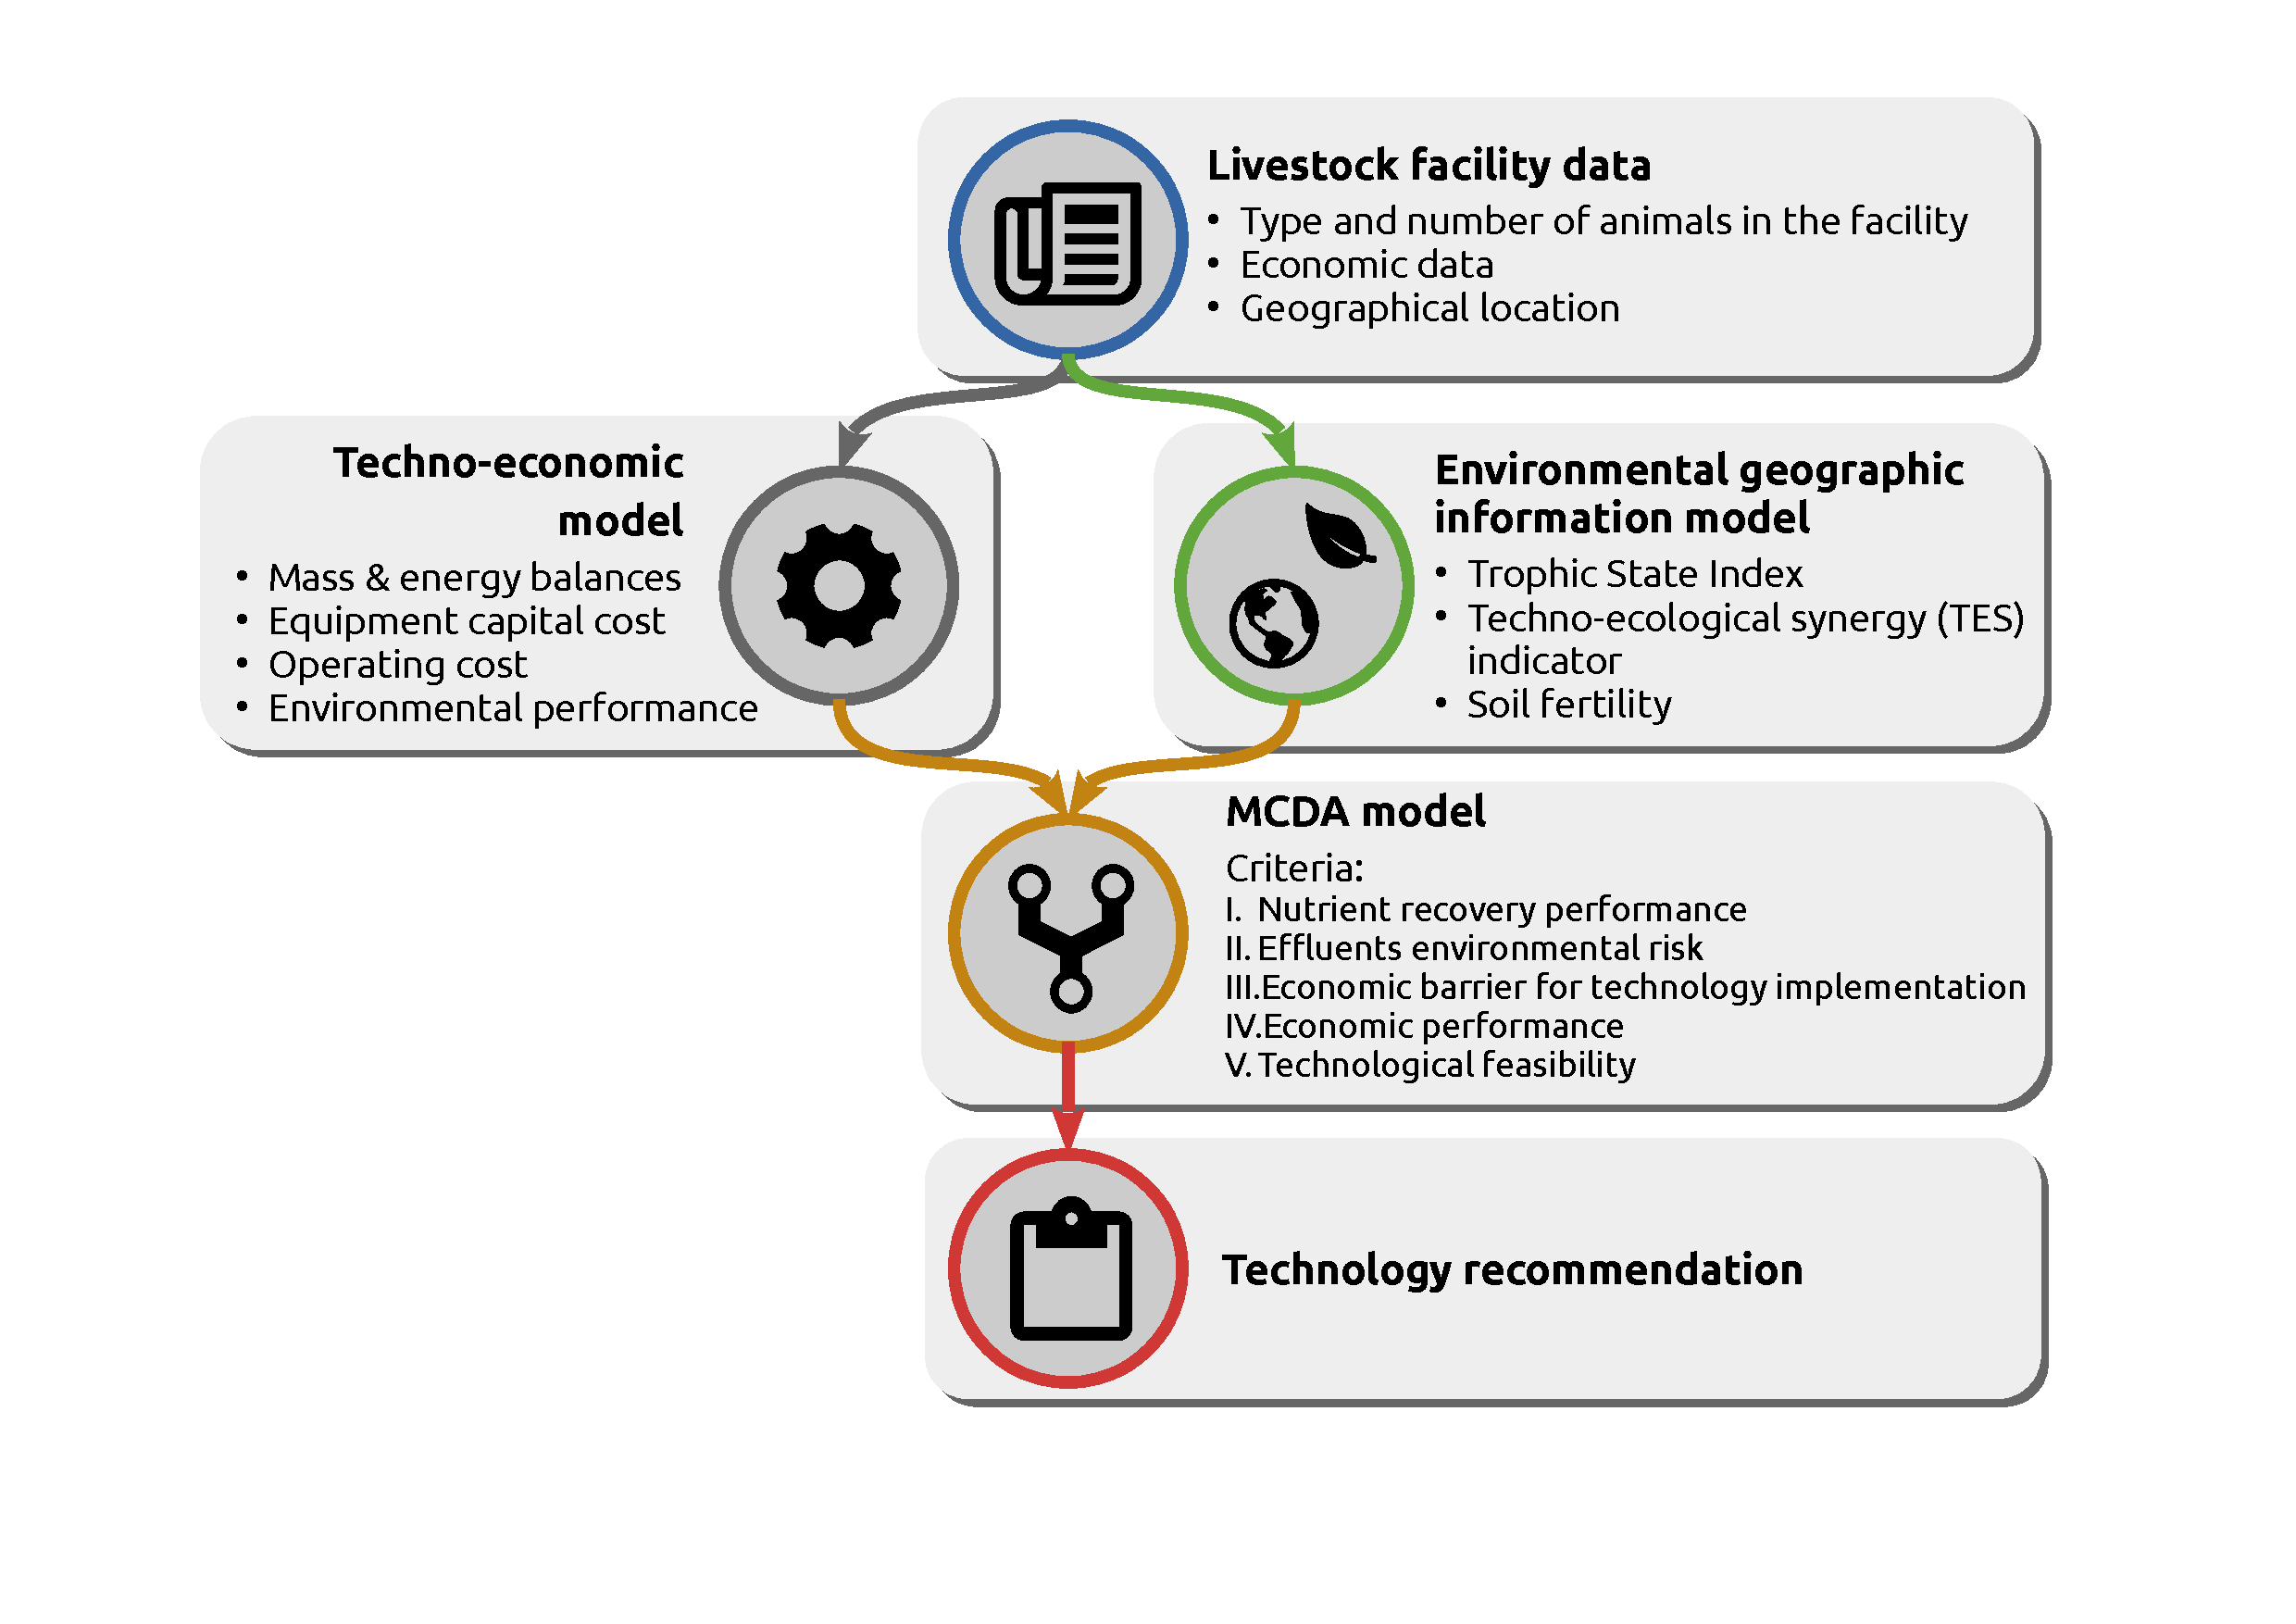
\includegraphics[width=0.85\linewidth, trim={3cm 4cm 4cm 1.5cm},clip]{tool_diagram_v4color.pdf} 
	\caption{Structure of the COW2NUTRIENT decision support framework for the assessment and selection of phosphorus recovery systems.}
	\label{fig:tool_diagram}
\end{figure}
%
%\subsection{User interface}
%A web-based user interface has been designed to make the tool easily accessible and intuitive for users. A detailed description of the tool development can be found in Section \ref{tool_develpoment}, while the design and mapping of the tool, as well as the user interface, can be found in Figs. 1. and 2 of the Supplementary Material. Additionally, a web-based tool allows the software to be centralized in a server, making the tool easier to maintain and update.
%
%\section{Tool development} \label{tool_develpoment}
%The proposed tool is divided in specialized modules performing different tasks: data entry, techno-economic module, environmental geographic information module, and multicriteria-decision analysis module, as shown in Figure \ref{fig:tool_diagram}. Stages for the anaerobic digestion of organic waste and biogas valorization, producing methane or electricity, can be optionally included, as well as the option to include a manure solid-liquid separation pre-processing stage if the facility is not equipped with this unit. 
%
%The output data returned to the user include environmental indicators for the vulnerability to phosphorus pollution of the watershed where the facility is located, mass balance and environmental performance of all processes evaluated, equipment and operating cost, and the recommendation of the most suitable nutrient recovery technology for the evaluated CAFO.
%
%\subsection{Data entry module}
%To capture the characteristics of each individual facility evaluated, the proposed tool is provided with a data entry interface where users can specify the geographic location (longitude and latitude) and the number of animals in the facility, including beef and dairy cattle, differentiating between adult animals, heifers, and calves, since each type of cattle has different manure generation rates and different manure composition. Data reported by the US Department of Agriculture (USDA) were considered for manure generation ratios \citep{Kellog2010} and for the composition of each type of cattle considered \citep{USDAHandbook}. These values are collected in Table 1 of the Supplementary Material. The optional integration of anaerobic digestion and biogas valorization processes, as well as solid-liquid separation pre-processing stage for the organic waste are also implemented in the data entry module. 
%
%For economic performance evaluation purposes, the values of the incentives received for phosphorus recovery (in the form of P credits), and for the generation of bio-based methane or electricity (in form of Renewable Energy Certificate (REC) and Renewable Identification Number (RIN) respectively) are predefined. Renewable Energy Credits is a mechanism implemented in the U.S. which guarantees that energy is generated from renewable sources, providing a system for trading produced renewable electricity. Each produced renewable megawatt-hour generates one REC, that can be sold separately from the electricity commodity itself and can be used to meet regulatory requirements by generators, trades, or end-users. On the other hand, RINs are identification numbers assigned toTo capture the characteristics of each individual facility evaluated batches of biofuel, allowing the tracking of its production, purchase, and final usage, which are associated with incentives for the generation bio-fuels.
%However, the values of these parameters can be customized to adapt the model to different economic scenarios. In addition, potential incentives to partially cover the capital cost of the nutrient recover process are also considered. The predefined value of the different incentives  are collected in Table 2 of the Suplemmentary Material. 

\subsection{Environmental geographic information model}
The environmental vulnerability to nutrient pollution of the area where the livestock facilities are located determines the preference (i.e., ranks the importance) of each criterion. 
%Three indicators are used to evaluate the eutrophication risk of each studied region: the average Trophic State Index (TSI) of the waterbodies \citep{carlson_trophic_1977}, the phosphorus saturation of soils as a result of nutrient legacy, which can lead the transport of phosphorus to waterbodies by run-off \citep{Espinoza2006}, and the balance between anthropogenic phosphorus releases and uptakes measured using the techno-ecological synergy (TES) metric \citep{TESmetric}.
Three indicators are used to evaluate the eutrophication risk of each region studied at subbasin spatial resolution. The trophic state of waterbodies is evaluated through the Trophic State Index
%(TSI)
\citep{carlson_trophic_1977}, determining their eutrophication level. The phosphorus saturation of soils, which can result in the transport of phosphorus to waterbodies by run-off, is evaluated through Mehlich 3 phosphorus concentration \citep{Espinoza2006}. Finally, the balance between phosphorus releases and uptakes from  anthropogenic activities is assessed through the techno-ecological synergy
%(TES)
metric \citep{TESmetric}, determining if there is a net accumulation or depletion of phosphorus in a region over time. 
The use of these three indicators makes it possible to determine if there exist an immediate risk of eutrophication in the region studied (eutrophized waterbodies), a long-term risk (moderate value of TSI, soils saturated by phosphorus, or phosphorus releases and uptakes from  anthropogenic activities unbalanced), or if there is no risk of eutrophication (phosphorus uptakes and releases are balanced). Detailed descriptions of the performed data analysis, and maps for the contiguous US are provided in Section 1 of the Supplementary Material.

\subsubsection{Spatial resolution}
%The environmental indicators considered by the framework are evaluated at a HUC8 watershed level.
A watershed is defined as the region draining all the streams and rainfall to a common waterbody, defining the geographic limits for the collection of runoff elements. US watersheds are designated by the US Geological Survey
%(USGS)
through the Hydrologic Unit Code (HUC) system. The HUC system divides the US into regions, subregions, basins, subbasins, watersheds, and subwatersheds. Each hydrologic unit of these six levels is identified hierarchically by a unique numeric code from 2 to 12 digits (i.e., HUC2 to HUC12).
The spatial resolution of this study is the contiguous United States at the subbasin level, defined by the HUC system at 8 digits (HUC8) \citep{HUC8}.

\subsubsection{Trophic State Index}
%The Trophic State Index (TSI) is a metric, proposed by \citet{carlson_trophic_1977} and used by the U.S. Environmental Protection Agency (US EPA) to determine the trophic status of waterbodies \citep{QAPP2012}. This index can be calculated using three parameters: concentration of chlorophyll-$\alpha$ (chl-$\alpha$), concentration of total phosphorus, and water turbidity measured through the Secchi depth. Correlations to compute the TSI from these parameters can be found in \citep{carlson_trophic_1977}. The TSI of a waterbody is scored in a range from zero to one hundred, which can be correlated with the oligotrophic, mesotrophic, eutrophic and hypereutrophic classes as shown in Table \ref{table:TSI_relation}. Among these trophic classes, oligotrophic, mesotrophic denote low and intermediate biomass productivity, while the last two are referred to waterbodies with high biological productivity and frequent algal blooms. To determine the Trophic State Index of lentic waters in the contiguous U.S., combined data for chl-$\alpha$ and total phosphorus concentrations retrieved from the National Lakes Assessments (NLA) carried out by the US EPA in the years 2007 and 2012 \citep{NLA2012, NLA2007}. For watersheds without reported data by the US EPA, no TSI value is assigned to them.
The Trophic State Index (TSI) is a metric proposed by \citet{carlson_trophic_1977}
%and used by the US Environmental Protection Agency (US EPA)
to determine the trophic status of waterbodies \citep{QAPP2012}. The TSI of a waterbody is scored in a range from 0 to 100 representing its throphic state, as shown in Table \ref{table:TSI_relation}. Oligotrophic and mesotrophic states denote low and intermediate biomass productivities, while eutrophic and hypereutrophic states are referred to waterbodies with high biological productivity and frequent algal blooms. Combined data for chl-$\alpha$ and total phosphorus concentrations retrieved from the National Lakes Assessments
%(NLA)
conducted by the US EPA in 2007 and 2012 \citep{NLA2012, NLA2007} is used to determine the Trophic State Index of lentic waters in the contiguous US. No TSI values were assigned to the watersheds without reported data. Correlations to estimate the TSI from chlorophyll-$\alpha$ and total phosphorus concentrations are collected in Section 1 of Supplementary Material.

\begin{table}[H]
	\centering
	\caption{Relation between TSI value and trophic class.}
	\label{table:TSI_relation}
	\begin{tabular}{@{}lllll@{}}
		\toprule
		{TSI}           & \textless 40 & 40-50       & 50-70     & \textgreater{}70 \\ \midrule
		{Trophic Class} & Oligotrophic & Mesotrophic & Eutrophic & Hypereutrophic   \\ \bottomrule
	\end{tabular}
\end{table}

\subsubsection{Techno-ecological synergy sustainability metric}
The techno-ecological synergy sustainability metric (TES) is an indicator proposed by \citet{TESmetric} to evaluate the fraction of net anthropogenic phosphorus releases, Eq. \ref{eq:TES}. 

\begin{align}
& V_{x} =\frac{\left(U_{x} - E_{x}\right)}{E_{x}} \label{eq:TES}
\end{align}

A negative value for TES indicator ($V_{x}$) indicates that the releases $\left(E_{x}\right)$ are larger than the uptake capacity of the evaluated system, $\left(U_{x}\right)$, and thus impacting in the ecosystems; while positive values reflects that the releases can be absorbed by the system without any harm. 

%Agricultural releases are a main source of human-based phosphorus releases due to the excessive use of synthetic fertilizers and livestock waste for nutrient supplementation in croplands \citep{Dzombak}. Since this work is limited to the assessment of agricultural phosphorus releases, other possible sources of phosphorus releases are not considered. Agricultural phosphorus releases have been estimated from data reported by the Nutrient Use Geographic Information System (NuGIS) project. Further information about the methodology used for the estimation of human-based phosphorus releases can be found in \citet{NuGIS}. 
%Agricultural releases are a main source of human-based phosphorus releases due to the excessive use of synthetic fertilizers and livestock waste for nutrient supplementation in croplands \citep{Dzombak}.
Phosphorus releases from agricultural activities have been estimated from data reported by the Nutrient Use Geographic Information System
%(NuGIS)
project. Since this work is limited to the assessment of agricultural phosphorus releases, other possible sources of phosphorus releases are not considered. Further information about the methodology used for the estimation of human-based phosphorus releases can be found in \citet{NuGIS}. 
%The anthropogenic phosphorus uptakes considered are those due to the crops grown in each watershed. In addition, phosphorus retained by wetlands is considered. Data from \citet{USDAWaste} is used to estimate the phosphorus uptakes of different crops, attending to their different phosphorus requirements and yield rates. To determine the crops in each area, the land cover uses are first determined using data from the US EPA EnviroAtlas database for the most recent year available (2011), differentiating between croplands, pasturelands, wetlands, and developed areas (urban areas) \citep{EnviroAtlas}. To estimate the distribution of crops in croplands, including corn, soybeans, small grains, cotton, rice, vegetables, orchards, greenhouse and other crops (i.e., fruits, sugar crops and oil crops) \citep{2017CensusofAgriculture}, data from the 2017 U.S. Census of Agriculture is used. In case of two or more crops were harvested from the same land during the year (double cropping), the area was counted for each crop. Since the data from the 2017 U.S. Census of Agriculture are published at HUC6 resolution, they have been reconciled to HUC8 level by the fraction of occupied area by each HUC8 watershed in the corresponding HUC6 watershed. The wetlands phosphorus uptake value assessed is 0.77 gP m$^{-2}$ year$^{-1}$, based on data reported by \citet{Kadlec}.
Anthropogenic phosphorus uptakes are those due to the crops grown in each watershed, including corn, soybeans, small grains, cotton, rice, vegetables, orchards, greenhouse and other crops (i.e., fruits, sugar crops, and oil crops). The estimation of the phosphorus uptakes is performed considering the different phosphorus requirements and yield rates of each crop, as well as the land cover and the crops distribution in each watershed. Data retrieved from \citet{2017CensusofAgriculture}, \citet{USDAHandbook}, and \citet{EnviroAtlas} is used for this purpose.

%Since different crops have different phosphorus uptakes and yield rates, the phosphorus uptakes are estimated for each type of crop in each watershed. Information available for the most recent year (2011) from the US EPA EnviroAtlas database is used to determine the land cover uses, accounting croplands, pasturelands, wetlands, and developed areas (urban areas) \citep{EnviroAtlas}. Data from the 2017 U.S. Census of Agriculture is used to determine the distribution of crops on croplands, including corn, soybeans, small grains, cotton, rice, vegetables, orchards, greenhouse and other crops (namely oil crops, sugar crops, and fruits) \citep{2017CensusofAgriculture}. Since the data from the 2017 U.S. Census of Agriculture are published at HUC6 resolution, they have been reconciled to HUC8 level by the fraction of occupied area by each HUC8 watershed in the corresponding HUC6 watershed. To determine the nutrients uptake of each type of crop, data from the USDA Waste Management Field Handbook is used \citep{USDAWaste}. The wetlands phosphorus uptake value assessed is 0.77 gP m$^{-2}$ year$^{-1}$, based on data reported by \citet{Kadlec}. More details about the procedure followed to estimate the phosphorus releases and emission can be found in the Supplementary Material

\subsubsection{Phosphorus saturation of soils}
%Datasets for samples from the soil A horizon published by the U.S. Geological Survey (USGS) in the ``Geochemical and Mineralogical Data for Soils of the Conterminous United States'' report was used to evaluate the concentration of total phosphorus along the contiguous U.S. \citep{SoilsUSGS}. This dataset allows to consider the legacy phosphorous continuously built-up in soils. However, since plants can just uptake an available fraction of total phosphorus, several standardized phosphorus soil tests, such as Olsen, Bray 1 and Mehlich 3 tests, have been developed to estimate P efficiency for crops. To relate total phosphorus and plant available phosphorus, correlations from Allen and Mallarino (2006) are used, Eq. \ref{eq:Mehlich3}, choosing Mehlich 3 (M3P) as P soil measure since is widely used and it is the P soil test least affected by changes in soil pH. Due to the lack of more complete studies, the correlations reported by \citet{AllenMallarino2006} for agricultural soils in Iowa are used. Therefore, the M3P estimates calculated for the contiguous U.S. must be considered as an exploratory effort to determine soil quality in an attempt to select the most suitable nutrients management technology according to the geographic environmental indicators. 
Phosphorus concentration in soil is used for the evaluation of the phosphorus legacy that is continuously built up in soils, providing a metric of soil quality. However, only a fraction of phosphorus is available for plants. To measure this phosphorus fraction available for plants, several standardized phosphorus soil tests have been proposed, including Olsen, Bray 1, and Mehlich 3 tests. Among them,  Mehlich 3 (M3P) has been selected as a measure of the concentration of P in soils since it is a widely used metric, and it is the P soil test least affected by changes in soil pH. To estimate the fraction of phosphorus available for plants from total phosphorus concentration data, a correlation developed by \citet{AllenMallarino2006} has been used, Eq. \ref{eq:Mehlich3}. It must be noted that this correlation has been developed for agricultural soils in Iowa, but due to the lack of studies in this topic, it has been used for soils throughout the contiguous US. Therefore, it must be considered as an exploratory effort to determine the phosphorus saturation in the US soils. Data reported by \citet{SoilsUSGS}
%the US Geological Survey
%(USGS)
%in the ``Geochemical and Mineralogical Data for Soils of the Conterminous United States'' report 
is used to evaluate the concentration of total phosphorus along the contiguous US.

\begin{align}
& \text{M3P} \ (\% \text{ over TP}) = \frac{4.698 \cdot 10^{-1}}{1+\left(\text{TotalP} \ (\text{mg}/\text{kg}) \cdot 1.336 \cdot 10^{-3}\right)^{-2.148}} \label{eq:Mehlich3}
\end{align}

The relationship between M3P test value and the quality of soil is shown in Table \ref{table:soil_fertility}. Soil fertility levels below optimum indicate that nutrient supplementation is needed to enhance the yield of crops, optimum values indicates that no nutrient supplementation is needed, and excessive soil fertility level indicate over-saturation of phosphorus in soil that can reach waterbodies by runoff \citep{Espinoza2006}.

\begin{table}[H]
	\centering
	\caption{Relationship between Mehlich 3 phosphorus and soil fertility level \protect\citep{Espinoza2006}.}
	\label{table:soil_fertility}
	\begin{tabular}{@{}cc@{}}
		\toprule
		Soil Fertility Level & M3P soil phosphorus concentration (ppm) \\ \midrule
		Very Low             & \textless{}16                           \\
		Low                  & 16-25                                   \\
		Medium               & 26-35                                   \\
		Optimum              & 36-50                                   \\
		Excessive            & \textgreater{}50                        \\ \bottomrule
	\end{tabular}
\end{table}

\subsection{Techno-economic model}
COW2NUTRIENT framework evaluates all the stages involved in the processing of manure for P recovery, from organic waste collection to the recovery of nutrients and other by-products such as electricity or biomethane, as represented in Fig \ref{fig:flowsheet}. In addition to the assessment of nutrient recovery systems, the framework is flexible to include anaerobic digestion, and the subsequent biogas valorization, for the production of methane or electricity. 
%This capability allows the evaluation of potential synergies between different processes for the treatment and valorization of manure, integrating the production of biogas-based products with the recovery of nutrients.
%, can be optionally included, as well as the option to include a manure solid-liquid separation pre-processing stage if the facility is not equipped with this unit. 
The techno-economic model is based on mass balances, thermodynamics, and chemical equilibria for each possible stage of the manure treatment process, i.e. manure conditioning, anaerobic digestion, biogas purification, biogas valorization, and phosphorus recovery. Preliminary design and sizing of equipment is performed to estimate the capital and operating expenses when no specific costs data are available. A detailed description of equipment design and sizing, as well as the correlations used for costs estimation, can be found in Section 2 of the Supplementary Material.

\begin{figure}[h]
	\centering
	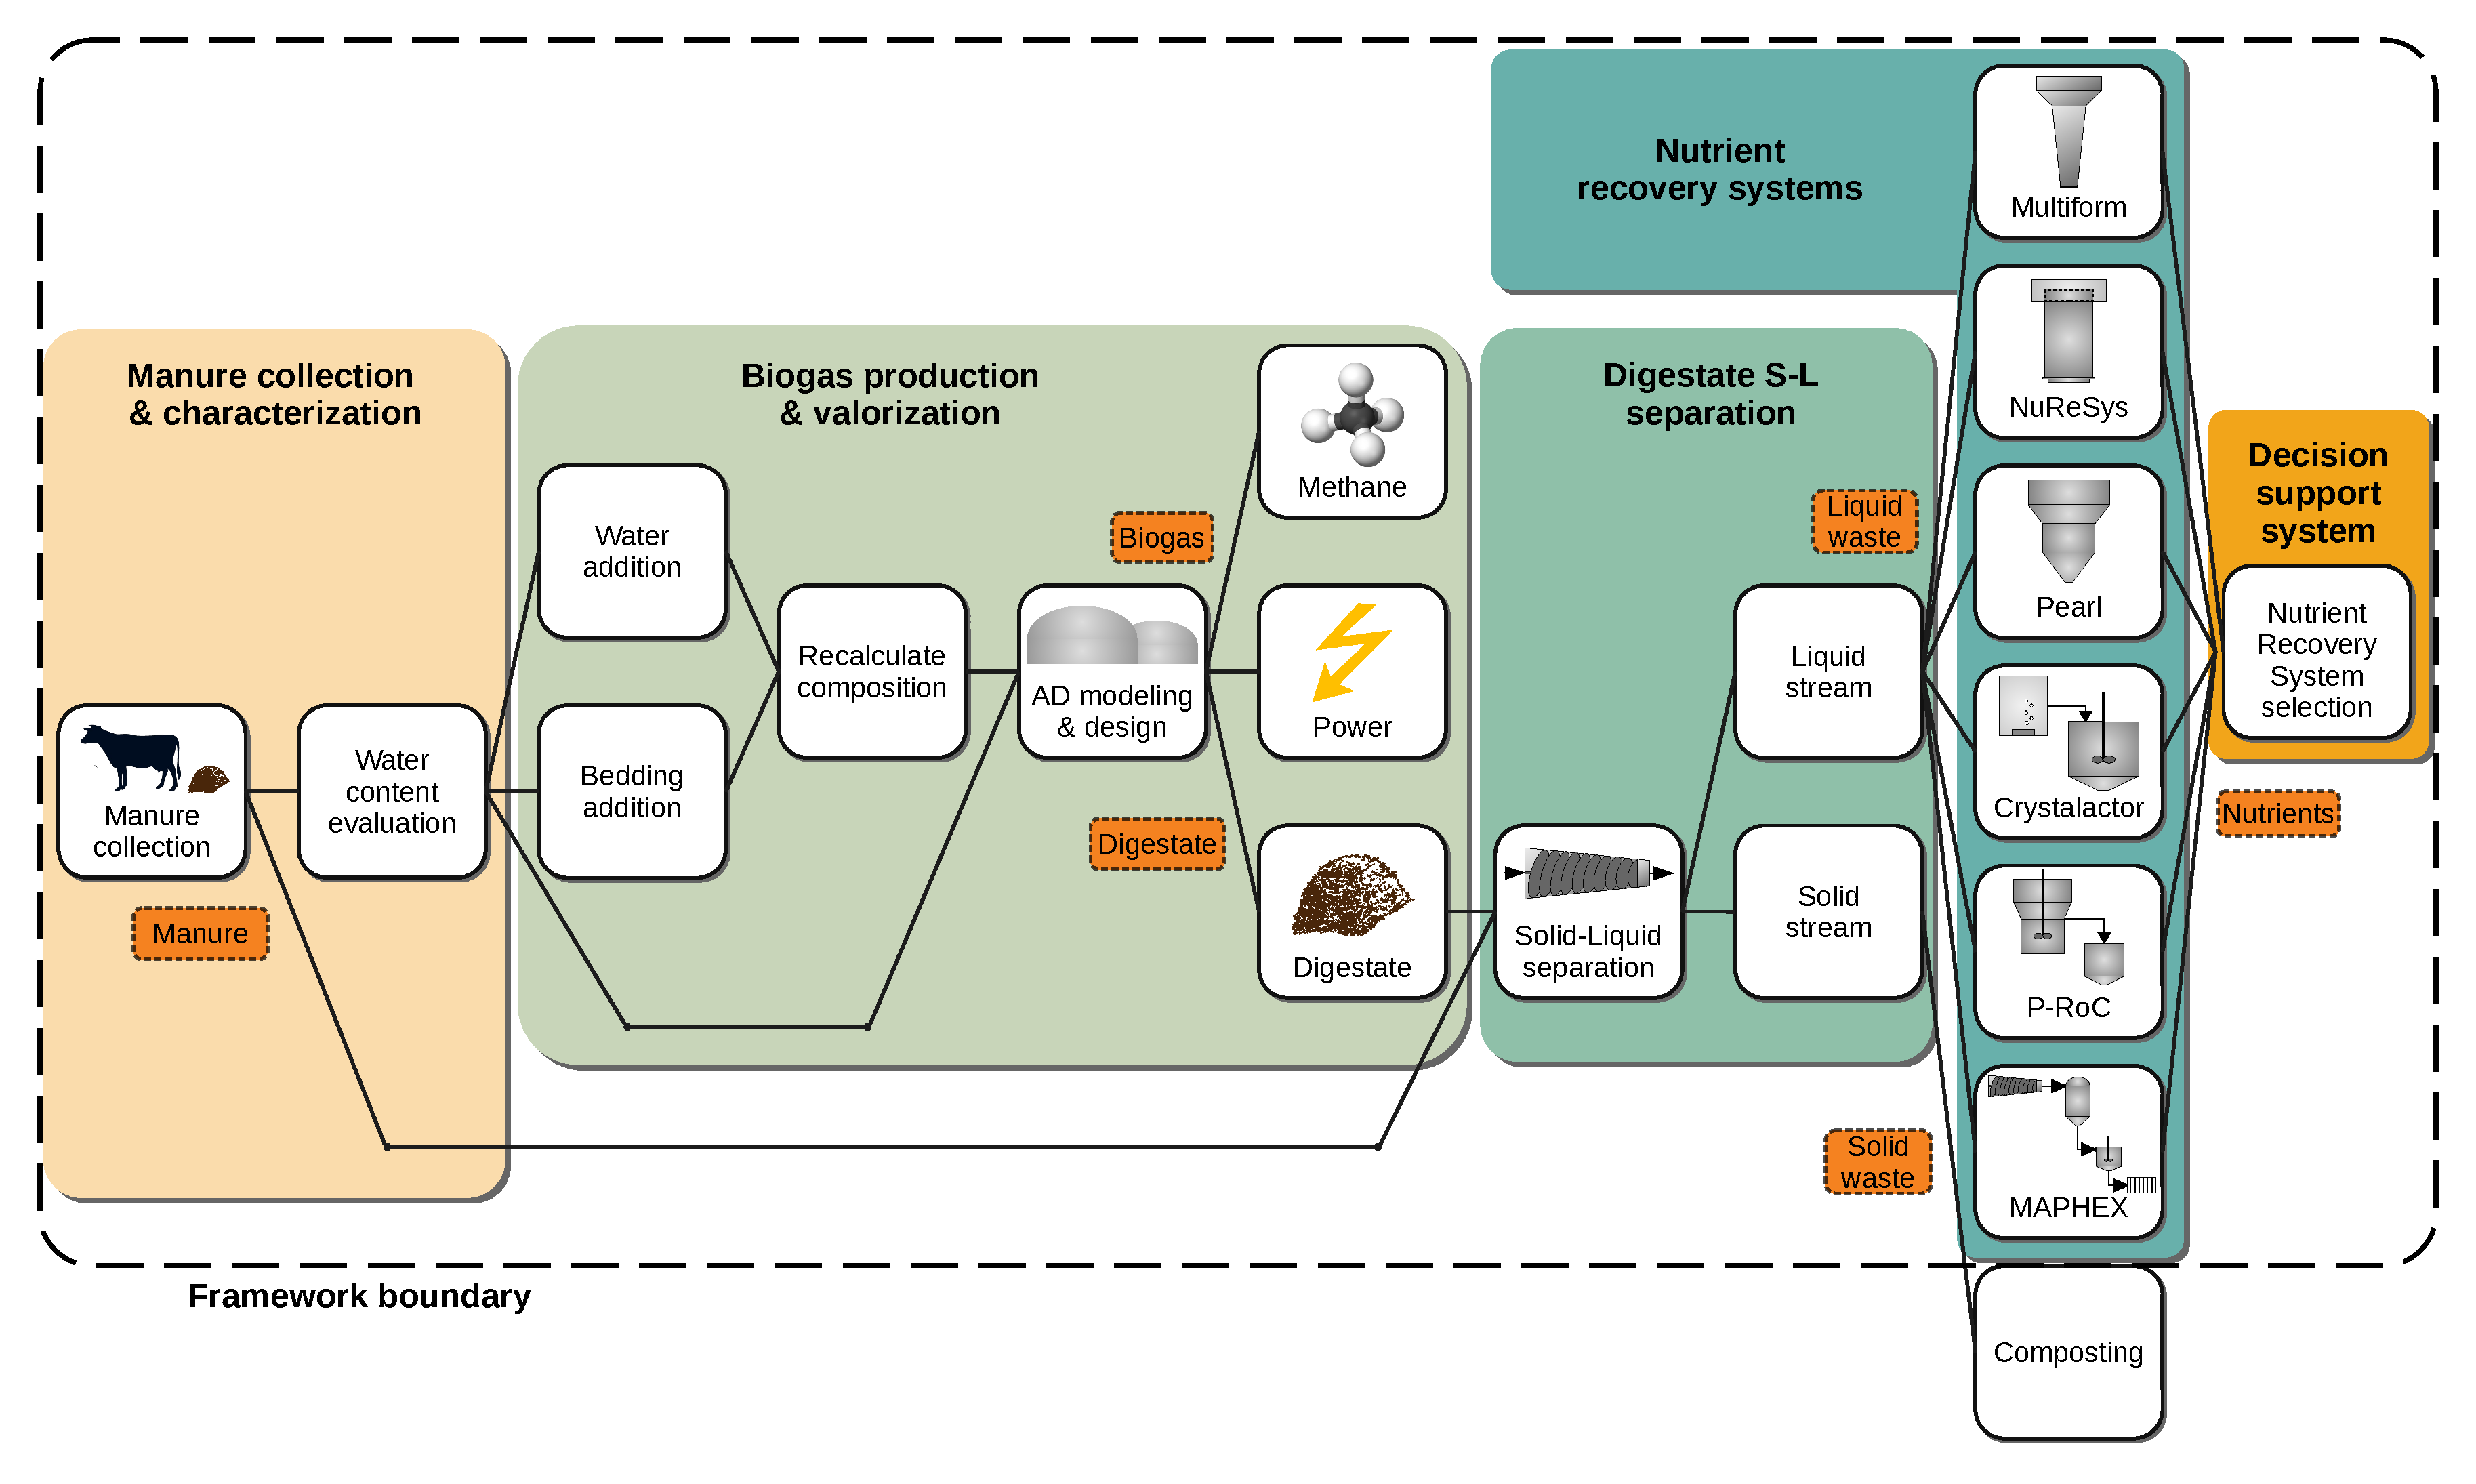
\includegraphics[width=0.95\linewidth, trim=1cm 1cm 1cm 1cm, clip]{Process_Flowsheet2.pdf} 
	\caption{Process flowsheet for manure management and phosphorus recovery stages included in COW2NUTRIENT.}
	\label{fig:flowsheet}
\end{figure}

\subsubsection{Manure conditioning}
It is considered that the collection of manure does not involve any cost, since CAFOs have manure collection systems already installed. All manure produced is assumed to be collected. If the anaerobic digestion (AD) stage is implemented, a preconditioning stage is considered to adjust the water content of the waste. US EPA determines that the content of total solids in manure should be less than 15\% \citep{AgSTARHandbook}, as shown in Figure 6S of the Supplementary Material. Therefore, additional water may be added to reduce the solids content in manure before the AD stage.
%
%\begin{figure}[H]
%	\centering
%	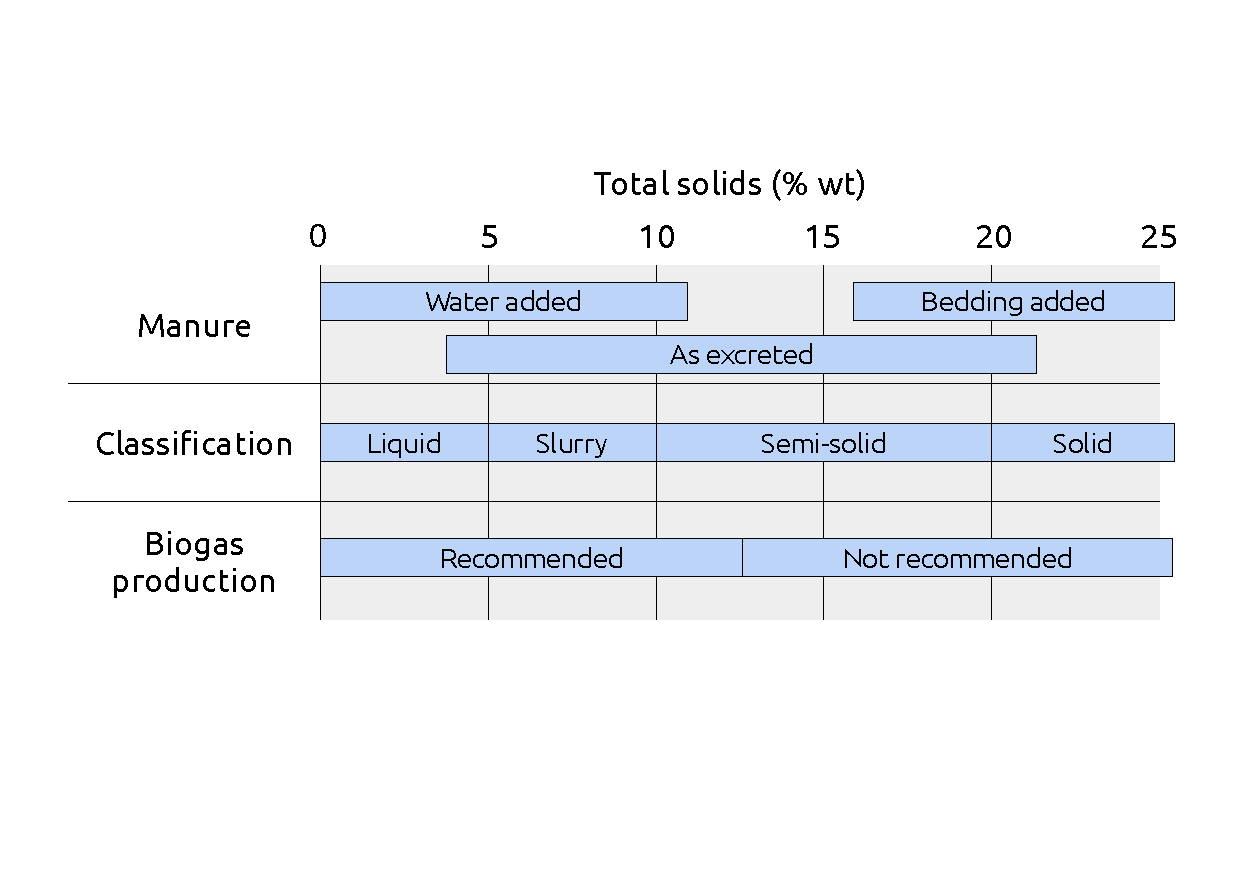
\includegraphics[width=0.7\linewidth, trim=1cm 4cm 1cm 2.5cm, clip]{water_manure_properties} 
%	\caption{Adequate manure properties for anaerobic digestion. Adapted from \protect\citet{AgSTARHandbook}.}
%	\label{fig:TS_max}
%\end{figure}

\subsubsection{Anaerobic digestion}
Anaerobic digestion is a microbiological process that breaks down organic matter in the absence of oxygen. It involves four stages, hydrolysis, acidogenesis, acetogenesis, and methanogenesis; producing a mixture of gases mainly composed of methane and carbon dioxide (biogas), and a decomposed organic substrate (digestate). The model of the anaerobic digester is formulated through the mass balances of the species involved in the production of biogas and digestate. A detailed description of the digester modeling can be found in \citet{Leon}. As a result of the AD process, a fraction of organic phosphorus and nitrogen are transformed in their inorganic forms. To evaluate the amount of organic nutrients transformed into inorganic phosphorus and nitrogen, data available in literature was considered, resulting in an increase of 24\% and 16\% over the original inorganic ammonia and phosphate respectively, as shown in Table 5S of the Supplementary Material.
%\citep{ADAS,Martin2,Alburquerque,Sorensen}. 
%Correlations to estimate the capital cost and operating and management costs (O\&M) as a function of the animal population of CAFOs were developed using data from the US EPA AgSTAR program \citep{AgSTAR2003} and the USDA \citep{USDA_OM} respectively. These are correlations, and further details regarding the cost estimation of the anaerobic digestor are collected in Section 2 of the Supplementary Material.
Correlations to estimate the capital cost
%, Eq. \ref{eq:inv_costs}, 
and operating and management costs (O\&M)
%, Eq. \ref{eq:OM_costs}, 
as a function of the animal population of CAFOs were developed using data from the US EPA AgSTAR program \citep{AgSTAR2003} and the USDA \citep{USDA_OM} respectively. We refer the reader to the Supplementary Material for further information.
%, as shown in Figure \ref{fig:AD_size_2cost}. It should be noted that O\&M cost does not include the capital cost amortization. Therefore, to estimate the total production cost, the annualized equipment cost has been added to the O\&M costs, Eq.  \ref{eq:OM_inv_costs}. The assumed equipment lifetime is 20 years.
%
%\begin{align} 
%	& \text{Installation cost (MM USD (2019))} = \left(4.271 \cdot 10^{-4} \cdot N_{animals}+0.127\right) \cdot 1.511 \label{eq:inv_costs}\\ \nonumber\\
%%	& \frac{\text{O\&M}} {\text{Installation cost}} \text{ ratio} = \frac{15858.710}{(1+\left(N_{animals} \cdot 13.917\right)^{1.461}} \label{eq:OM_costs}\\ \nonumber\\
%	& \frac{\text{O\&M}} {\text{Installation cost}} \text{ ratio} = \frac{15.858\cdot 10^{3}}{(1+\left(N_{animals} \cdot 13.917\right)^{1.461}} \label{eq:OM_costs}\\ \nonumber\\
%	& \text{Operating cost} = \text{O\&M costs} + \frac{\text{Investment cost}}{\text{Plant lifetime}} \label{eq:OM_inv_costs}
%\end{align}
%
%\begin{figure}[H]
%	\centering
%	\begin{subfigure}[t]{0.48\textwidth}
%		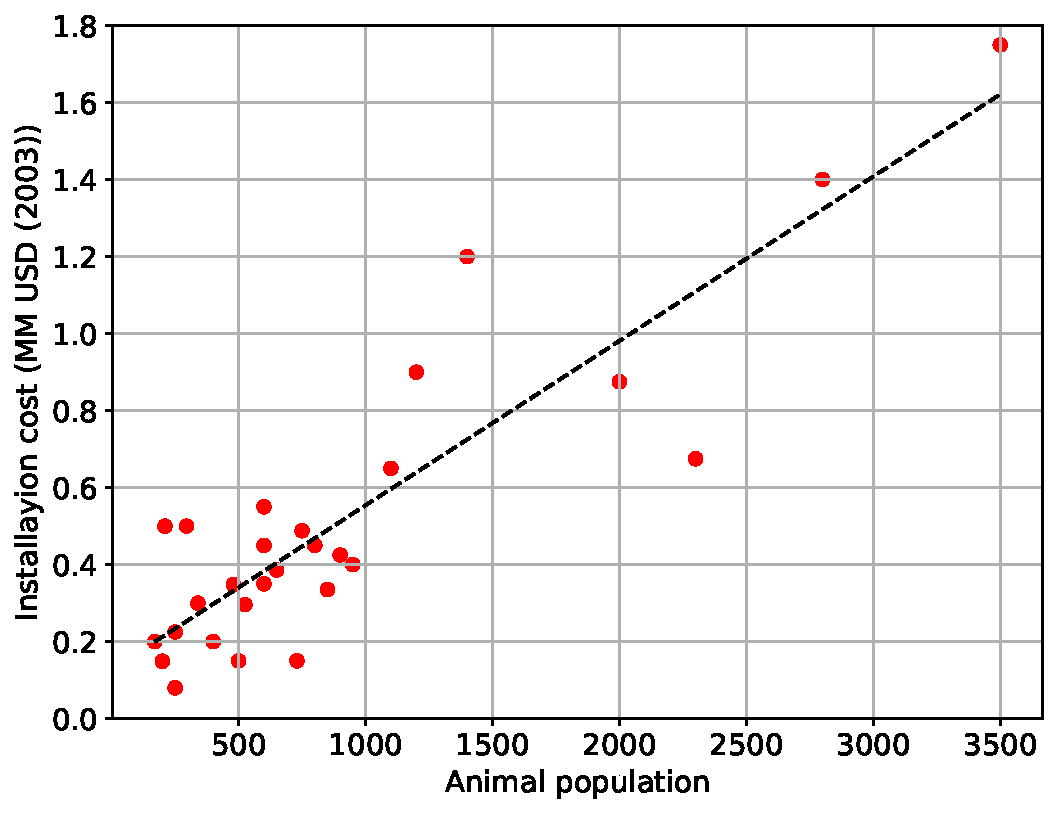
\includegraphics[width=\textwidth, trim={0cm 0cm 0cm 0cm},clip]{AD_size_cost.pdf}
%		\caption{Cost of AD units as a function of the number of animals (cattle). Data from \citet{AgSTAR2003}.}
%		\label{fig:AD_size_cost}
%	\end{subfigure}
%	\quad
%	\begin{subfigure}[t]{0.48\textwidth}
%		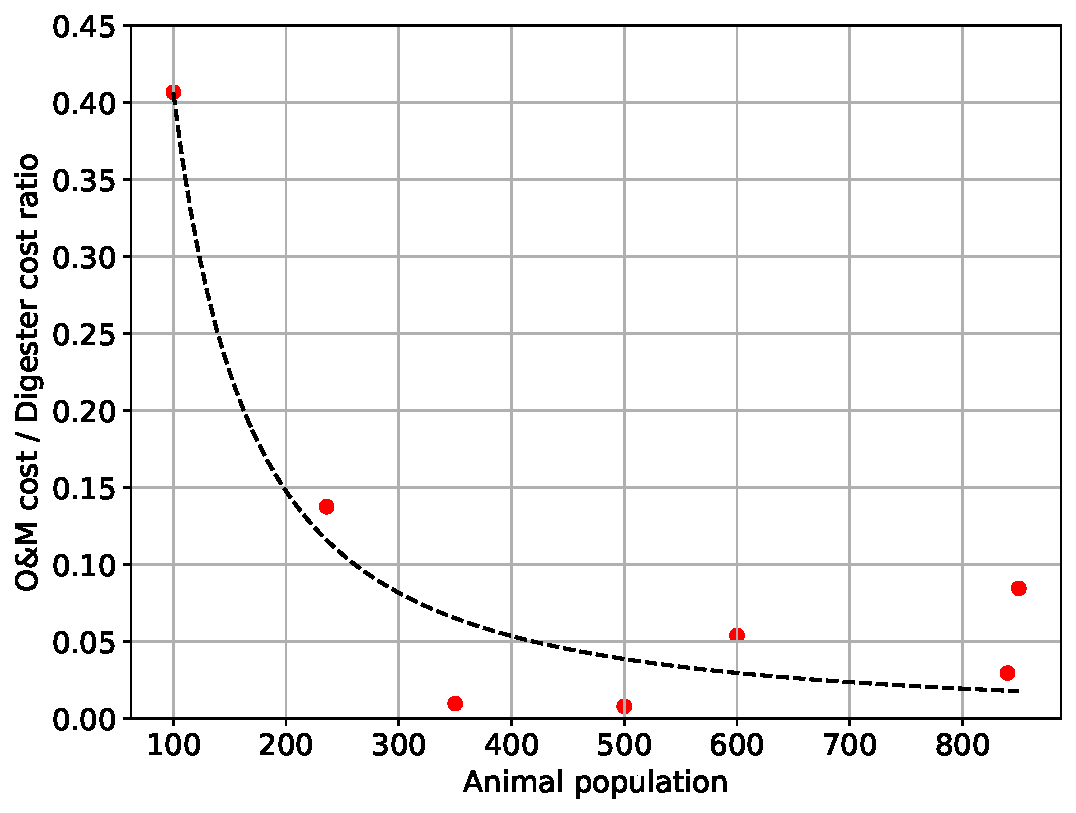
\includegraphics[width=\textwidth]{AD_size_OM_Unit_cost.pdf} 
%		\caption{O\&M costs as a function of the number of animals (cattle). Data from \citet{USDA_OM}.}
%		\label{fig:AD_size_OM_Unit_cost}
%	\end{subfigure}
%	
%	\caption{Correlations between AD capital and O\&M costs, and the number of cattle in the livestock facility.}
%	\label{fig:AD_size_2cost}
%\end{figure}

\subsubsection{Biogas purification}
Before transforming biogas into marketable products, a purification stage has to be carried out to remove H\textsubscript{2}S, H\textsubscript{2}O, and NH\textsubscript{3}. The removal of H\textsubscript{2}S is performed in a bed of ferric oxide through the production of Fe\textsubscript{2}S\textsubscript{3} operating at a temperature range of 25-50\textdegree C. The bed regeneration is carried out using oxygen to produce elemental sulfur and ferric oxide (Fe\textsubscript{2}O\textsubscript{3}). Water and ammonia are adsorbed using a pressure swing adsorption system (PSA) with zeolite 5A as adsorbent material, operating at low temperature (25\textdegree C) and moderate pressure (4.5 bar). The assumed recovery for NH\textsubscript{3} and H\textsubscript{2}O is 100\%. For further details about the modeling of the biogas purification stage, we refer the reader to previous works \citep{Leon, MartinHernandez}.

\subsubsection{Biogas valorization}
Two final added value products have been considered, methane and electricity, since they can be obtained through relatively simple processes and there exists developed markets for them.

\paragraph{Methane production}
The process considered for methane production is the removal of CO\textsubscript{2} using a PSA system with a bed of zeolite 5A, since this process was demonstrated as the optimal biogas upgrading process by \citet{MartinHernandez2020}, where further details about the modeling of the PSA system can be found.

\paragraph{Electricity production}
Electricity is produced from biogas through a gas turbine. A Brayton cycle consisting of double-stage compression system, one for the air stream and one for the biogas stream, is considered. Polytropic compression is assumed, with a polytropic index of 1.4 and an efficiency of 85\% \citep{moran2010fundamentals}. The adiabatic combustion of methane contained in the biogas is assumed, with a pre-heating of the biogas-air mixture, considering the combustion chamber as an adiabatic furnace. An air excess of 20\% with respect to the stoichiometric needs, and 100\% conversion of the reaction are assumed. Further details for electricity production can be found in \citet{MartinHernandez}.

\subsubsection{Solid-liquid separation}
Nutrients contained in organic waste (manure or digestate, depending on whether AD is carried out or not) are present in both organic and inorganic forms. Organic nutrients are chemically bonded to carbon, and they have to be converted into their inorganic forms through a mineralization process to be available for the vegetation to grow. Organic nutrients are mainly contained in the solid phase of organic waste. Inorganic nutrients are water soluble, and they are mostly present in the liquid phase, or bounded to soluble minerals. They are immediately available to plants, including algae involved during the occurrence of HABs. To recover the inorganic fraction of nutrients, a solid-liquid separation stage is implemented, keeping the inorganic nutrients in the liquid stage, which will be further processed, and the organic nutrients in the solid phased, which can be composted to mineralize nitrogen and phosphorus and be further used as fertilizers. The study of organic waste composting is out of the scope of this work.

Based on the evaluation reported by \citet{MollerSLsep}, a screw press is the technology selected to carry out the solid-liquid separation stage since it is the most cost-efficient
%liquid-solid 
equipment. The partition coefficients for the different components are shown in Table 6S of the Supplementary Material. Assuming the discretization of units due to the commercial sizes available, the investment and operating costs for the screw press equipment are presented in Figure 9S of the Supplementary Material.

\subsubsection{Phosphorus recovery}
The technologies to recover inorganic phosphorus can be classified in three categories: struvite-based phosphorus recovery, calcium precipitates-based phosphorus recovery, and physical separation systems. Table \ref{table:techs_description} shows the classification and characteristics of the evaluated technologies. Regarding struvite-based systems, the formation of struvite has been widely described in the  literature, mainly focused on phosphorus recovery from wastewater \citep{rahaman_modeling_2014, Battistoni}. 
%Experimental data available to evaluate the efficiency and feasibility of P recovery through struvite formation are usually developed for municipal wastewater. 
However, cattle organic waste shows some characteristics that hinder struvite formation, including high ionic strength, which reduces the effective concentration of ions; and the presence of calcium ions competing for phosphate ions \citep{Yan2016}, which inhibits a selective recovery by phosphorus precipitation. The high variability in the manure composition, as a function of the geographic area, the animal feed, etc., represents an additional challenge for nutrient recovery \citep{Tao}. Therefore, specific correlations for livestock waste to estimate the molar fraction of $\text{PO}_{4}^{3-}$ and $\text{Ca}^{2+}$ recovered as struvite as a function of the amount of calcium contained in the waste were developed in a previous work \citep{MartinStruvite}. 

Among the different products obtained by the different processes, only struvite generates income. Calcium precipitates lacks of a well-established market as fertilizer, and therefore no sales of this product are considered. MAPHEX produces an organic solid rich in nutrients, but with a lower nutrient density compared with struvite, hindering transportation of this product and decreasing its market value. Therefore, we have assumed that no income is obtained from this product. Nevertheless, the recovered products allow phosphorus distribution from CAFO releases to phosphorus-deficient areas.
%, Eqs. \ref{eq:sigmoidal_Ca_StrYield} to \ref{eq:sigmoidal_CaCaCO3}, where $x_{Ca^{2+}:PO_{4}^{3-}}$ refers to the $\text{Ca}^{2+}/\text{PO}_{4}^{3-} \ \text{molar ratio}$, $x_{struvite \left(PO_{4}^{3-}\right) }$ is the fraction of phosphorus as phosphate recovered as struvite, and $x_{hydroxyapatite \left(Ca^{2+}\right)}$ and $x_{CaCO_{3} \left(Ca^{2+}\right)}$ are the fraction of calcium recovered as hydroxyapatite and calcium carbonate respectively. 

All technologies considered are at or near commercial stage. We note that, for all the technologies evaluated, the installation of several P recovery units in parallel arrangement is considered if the amount of waste to be processed exceeds the treatment capacity of the system. The description of the processes, and the correlations used to estimate the struvite formed, equipment cost, and operating costs are collected in the Section 2.2.4 of the Supplementary Material.
%
%\begin{align}
%&x_{Struvite}= \frac{0.798}{1+\left(x_{Ca^{2+}:PO_{4}^{3-}} \cdot 0.576\right)^{2.113}} \cdot 100 \label{eq:sigmoidal_Ca_StrYield} \\
%\nonumber \\
%\begin{split}
%& x_{Hydroxyapatite} =\big(-4.321 \cdot 10^{-2} \cdot x_{Ca^{2+}:PO_{4}^{3-}}^{2} + 0.313 \cdot x_{Ca^{2+}:PO_{4}^{3-}} \\& \hspace{7.8cm} - 3.619 \cdot 10^{-2} \big) \cdot 100 \label{eq:sigmoidal_Ca_HAP}
%\end{split}
%\\
%\nonumber \\
%&  x_{CaCO_{3}} = \frac{1.020}{1+\left(x_{Ca^{2+}:PO_{4}^{3-}} \cdot 0.410 \right)^{1.029}} \cdot 100 \label{eq:sigmoidal_CaCaCO3}
%\end{align}

%\begin{table}[]
%	\centering
%	\caption{Description of phosphorus recovery technologies systems by COW2NUTRIENT framework.}
%	\label{table:techs_description}
%	% Please add the following required packages to your document preamble:
%	% \US EPAckage{booktabs}
%	\resizebox{\columnwidth}{!}{
%	\begin{tabular}{@{}ccccc@{}}
%		\toprule
%		Technology   & Company                                                                       & Technology type                                                            & \begin{tabular}[c]{@{}c@{}}Technology\\ readiness level\end{tabular} & \begin{tabular}[c]{@{}c@{}}Phosphorus recovery\\ efficiency (\%)\end{tabular} \\ \midrule
%		Multiform    & Multiform Harvest                                                             & Struvite-based                                                             & 9                                                                    & Eq. \ref{eq:sigmoidal_Ca_StrYield}                         \\ \\
%		Crystalactor & \begin{tabular}[c]{@{}c@{}}Royal Haskoning\\ DHV\end{tabular}                 & Struvite-based                                                             & 9                                                                    & Eq. \ref{eq:sigmoidal_Ca_StrYield}                        \\ \\
%		NuReSys      & \begin{tabular}[c]{@{}c@{}}Nutrient Recovery\\ Systems\end{tabular}           & Struvite-based                                                             & 9                                                                    & Eq. \ref{eq:sigmoidal_Ca_StrYield}                         \\ \\
%		Pearl        & Ostara                                                                        & Struvite-based                                                             & 9                                                                    & Eq. \ref{eq:sigmoidal_Ca_StrYield}                         \\ \\
%		P-RoC        & \begin{tabular}[c]{@{}c@{}}Karlsruhe Institute\\ of Technology\end{tabular}   & \begin{tabular}[c]{@{}c@{}}Calcium \\ precipitates-based\end{tabular}      & 6                                                                    & 60                                                                            \\ \\
%		MAPHEX       & \begin{tabular}[c]{@{}c@{}}University of Pennsylvania\\ and USDA\end{tabular} & \begin{tabular}[c]{@{}c@{}}Modular phases\\ separation system\end{tabular} & 7                                                                    & 90                                                                            \\ \bottomrule
%	\end{tabular}}
%\end{table}

%\begin{table}[]
%	\centering
%	\caption{Description of phosphorus recovery technologies systems by COW2NUTRIENT framework. $x_{Ca^{2+}:PO_{4}^{3-}}$ refers to the $\text{Ca}^{2+}/\text{PO}_{4}^{3-} \ \text{molar ratio}$.}
%	\label{table:techs_description}
%	% Please add the following required packages to your document preamble:
%	% \US EPAckage{booktabs}
%	\resizebox{\columnwidth}{!}{
%		\begin{tabular}{@{}ccccc@{}}
%			\toprule
%			Technology   & Company                                                                       & Technology type                                                            & \begin{tabular}[c]{@{}c@{}}Technology\\ readiness level\end{tabular} & \begin{tabular}[c]{@{}c@{}}Phosphorus recovery\\ efficiency (\%)\end{tabular}  \\ \midrule
%			Multiform    & Multiform Harvest                                                             & Struvite-based                                                             & 9                                                                    & $\frac{0.798 \cdot 100}{1+\left(x_{Ca^{2+}:PO_{4}^{3-}} \cdot 0.576\right)^{2.113}}$                         \\ \\
%			Crystalactor & \begin{tabular}[c]{@{}c@{}}Royal Haskoning\\ DHV\end{tabular}                 & Struvite-based                                                             & 9                                                                    & $\frac{0.798 \cdot 100}{1+\left(x_{Ca^{2+}:PO_{4}^{3-}} \cdot 0.576\right)^{2.113}}$                            \\ \\
%			NuReSys      & \begin{tabular}[c]{@{}c@{}}Nutrient Recovery\\ Systems\end{tabular}           & Struvite-based                                                             & 9                                                                    & $\frac{0.798 \cdot 100}{1+\left(x_{Ca^{2+}:PO_{4}^{3-}} \cdot 0.576\right)^{2.113}}$                            \\ \\
%			Pearl        & Ostara                                                                        & Struvite-based                                                             & 9                                                                    & $\frac{0.798 \cdot 100}{1+\left(x_{Ca^{2+}:PO_{4}^{3-}} \cdot 0.576\right)^{2.113}}$                               \\ \\
%			P-RoC        & \begin{tabular}[c]{@{}c@{}}Karlsruhe Institute\\ of Technology\end{tabular}   & \begin{tabular}[c]{@{}c@{}}Calcium \\ precipitates-based\end{tabular}      & 6                                                                    & 60                                                                            \\ \\
%			MAPHEX       & \begin{tabular}[c]{@{}c@{}}University of Pennsylvania\\ and USDA\end{tabular} & \begin{tabular}[c]{@{}c@{}}Modular phases\\ separation system\end{tabular} & 7                                                                    & 90                                                                            \\ \bottomrule
%	\end{tabular}}
%\end{table}

\begin{sidewaystable}[]
	\centering
	\caption{Description of phosphorus recovery technologies systems by COW2NUTRIENT framework. $x_{Ca^{2+}:PO_{4}^{3-}}$ refers to the $\text{Ca}^{2+}/\text{PO}_{4}^{3-} \ \text{molar ratio}$. $n_i$ denotes the number of units of the technology $i$ installed.}
	\label{table:techs_description}
	% Please add the following required packages to your document preamble:
	% \US EPAckage{booktabs}
	\resizebox{\columnwidth}{!}{
		\begin{tabular}{@{}ccccccccc@{}}
			\toprule
			Technology   & Company                                                                       & Technology type                                                            & \begin{tabular}[c]{@{}c@{}}Technology\\ readiness level\end{tabular} & \begin{tabular}[c]{@{}c@{}}Phosphorus recovery\\ efficiency (\%)\end{tabular} & 
			\begin{tabular}[c]{@{}c@{}}Treatment capacity\\ $\left(\frac{\text{kg\textsubscript{P-PO4}}}{\text{day} \cdot \text{unit}}\right)$ \end{tabular} & \begin{tabular}[c]{@{}c@{}}CAPEX\\ $\left(\frac{\text{MM USD}}{\text{unit}}\right)$ \end{tabular} & \begin{tabular}[c]{@{}c@{}} OPEX\\ $\left(\frac{\text{USD}}{\text{\text{kg\textsubscript{P-PO4}}}}\right)$ \end{tabular} & Reference \\ \midrule
			Multiform    & Multiform Harvest                                                             & Struvite-based                                                             & 9                                                                    & $\frac{0.798 \cdot 100}{1+\left(x_{Ca^{2+}:PO_{4}^{3-}} \cdot 0.576\right)^{2.113}}$   &38.5       &       1.1 &   15.42 & 1  \\ \\
			
			Crystalactor & \begin{tabular}[c]{@{}c@{}}Royal Haskoning\\ DHV\end{tabular}                 & Struvite-based                                                             & 9                                                                    & $\frac{0.798 \cdot 100}{1+\left(x_{Ca^{2+}:PO_{4}^{3-}} \cdot 0.576\right)^{2.113}}$     & 137.7           &    $2.3 + 0.71 \cdot n_{\text{Crystalactor}}$      &  2.12 & 2  \\ \\
			
			NuReSys      & \begin{tabular}[c]{@{}c@{}}Nutrient Recovery\\ Systems\end{tabular}           & Struvite-based                
			& 9                                                                    & $\frac{0.798 \cdot 100}{1+\left(x_{Ca^{2+}:PO_{4}^{3-}} \cdot 0.576\right)^{2.113}}$   & 204.0          &     1.38   &   6.22 &  1 \\ \\
			
			Pearl 500       & Ostara                                                                        & Struvite-based                                                             & 9                                                                    & $\frac{0.798 \cdot 100}{1+\left(x_{Ca^{2+}:PO_{4}^{3-}} \cdot 0.576\right)^{2.113}}$            &         65.0    &  2.3 &  7.54 & 3 \\ \\
		
			Pearl 2K       & Ostara                                                                        & Struvite-based                                                             & 9                                                                    & $\frac{0.798 \cdot 100}{1+\left(x_{Ca^{2+}:PO_{4}^{3-}} \cdot 0.576\right)^{2.113}}$            &      250.0   &   3.1  & 7.54 & 1 \\ \\
		
			Pearl 10K       & Ostara                                                                        & Struvite-based                                                             & 9                                                                    & $\frac{0.798 \cdot 100}{1+\left(x_{Ca^{2+}:PO_{4}^{3-}} \cdot 0.576\right)^{2.113}}$            &         1250.0    &  10.0 &  7.54 & 4 \\ \\
		
			P-RoC        & \begin{tabular}[c]{@{}c@{}}Karlsruhe Institute\\ of Technology\end{tabular}   & \begin{tabular}[c]{@{}c@{}}Calcium \\ precipitates-based\end{tabular}      & 6                                                                    & 60                      & 24.3     &  \begin{tabular}[c]{@{}c@{}}Tailored design based\\on waste flow processed. \\ See Section 2.2.4.4 of \\ Supplementary Material.	\end{tabular}   &     23.22 - 167.8  & 5  \\ \\
		
			MAPHEX       & \begin{tabular}[c]{@{}c@{}}University of Pennsylvania\\ and USDA\end{tabular} & \begin{tabular}[c]{@{}c@{}}Modular phases\\ separation system\end{tabular} & 7                                                                    & 90                                                      & 18.5   &   0.3    &    110.8  & 6, 7  \\ \bottomrule
	\end{tabular}}
	\begin{tablenotes}
		\footnotesize
		\item 1: \citet{Pearl2Kcost2}
		\item 2: \citet{egle_phosphorus_2016}
		\item 3: \citet{Pearl500cost1}
		\item 4: \citet{Pearl10Kcost1}
		\item 5: \citet{ehbrecht_p-recovery_2011}
		\item 6: \citet{church_novel_2016}
		\item 7: \citet{church_versatility_2018}
	\end{tablenotes}
\end{sidewaystable}

%\begin{figure}[H]
%	\centering
%	%	\begin{subfigure}[t]{0.5\linewidth}
%	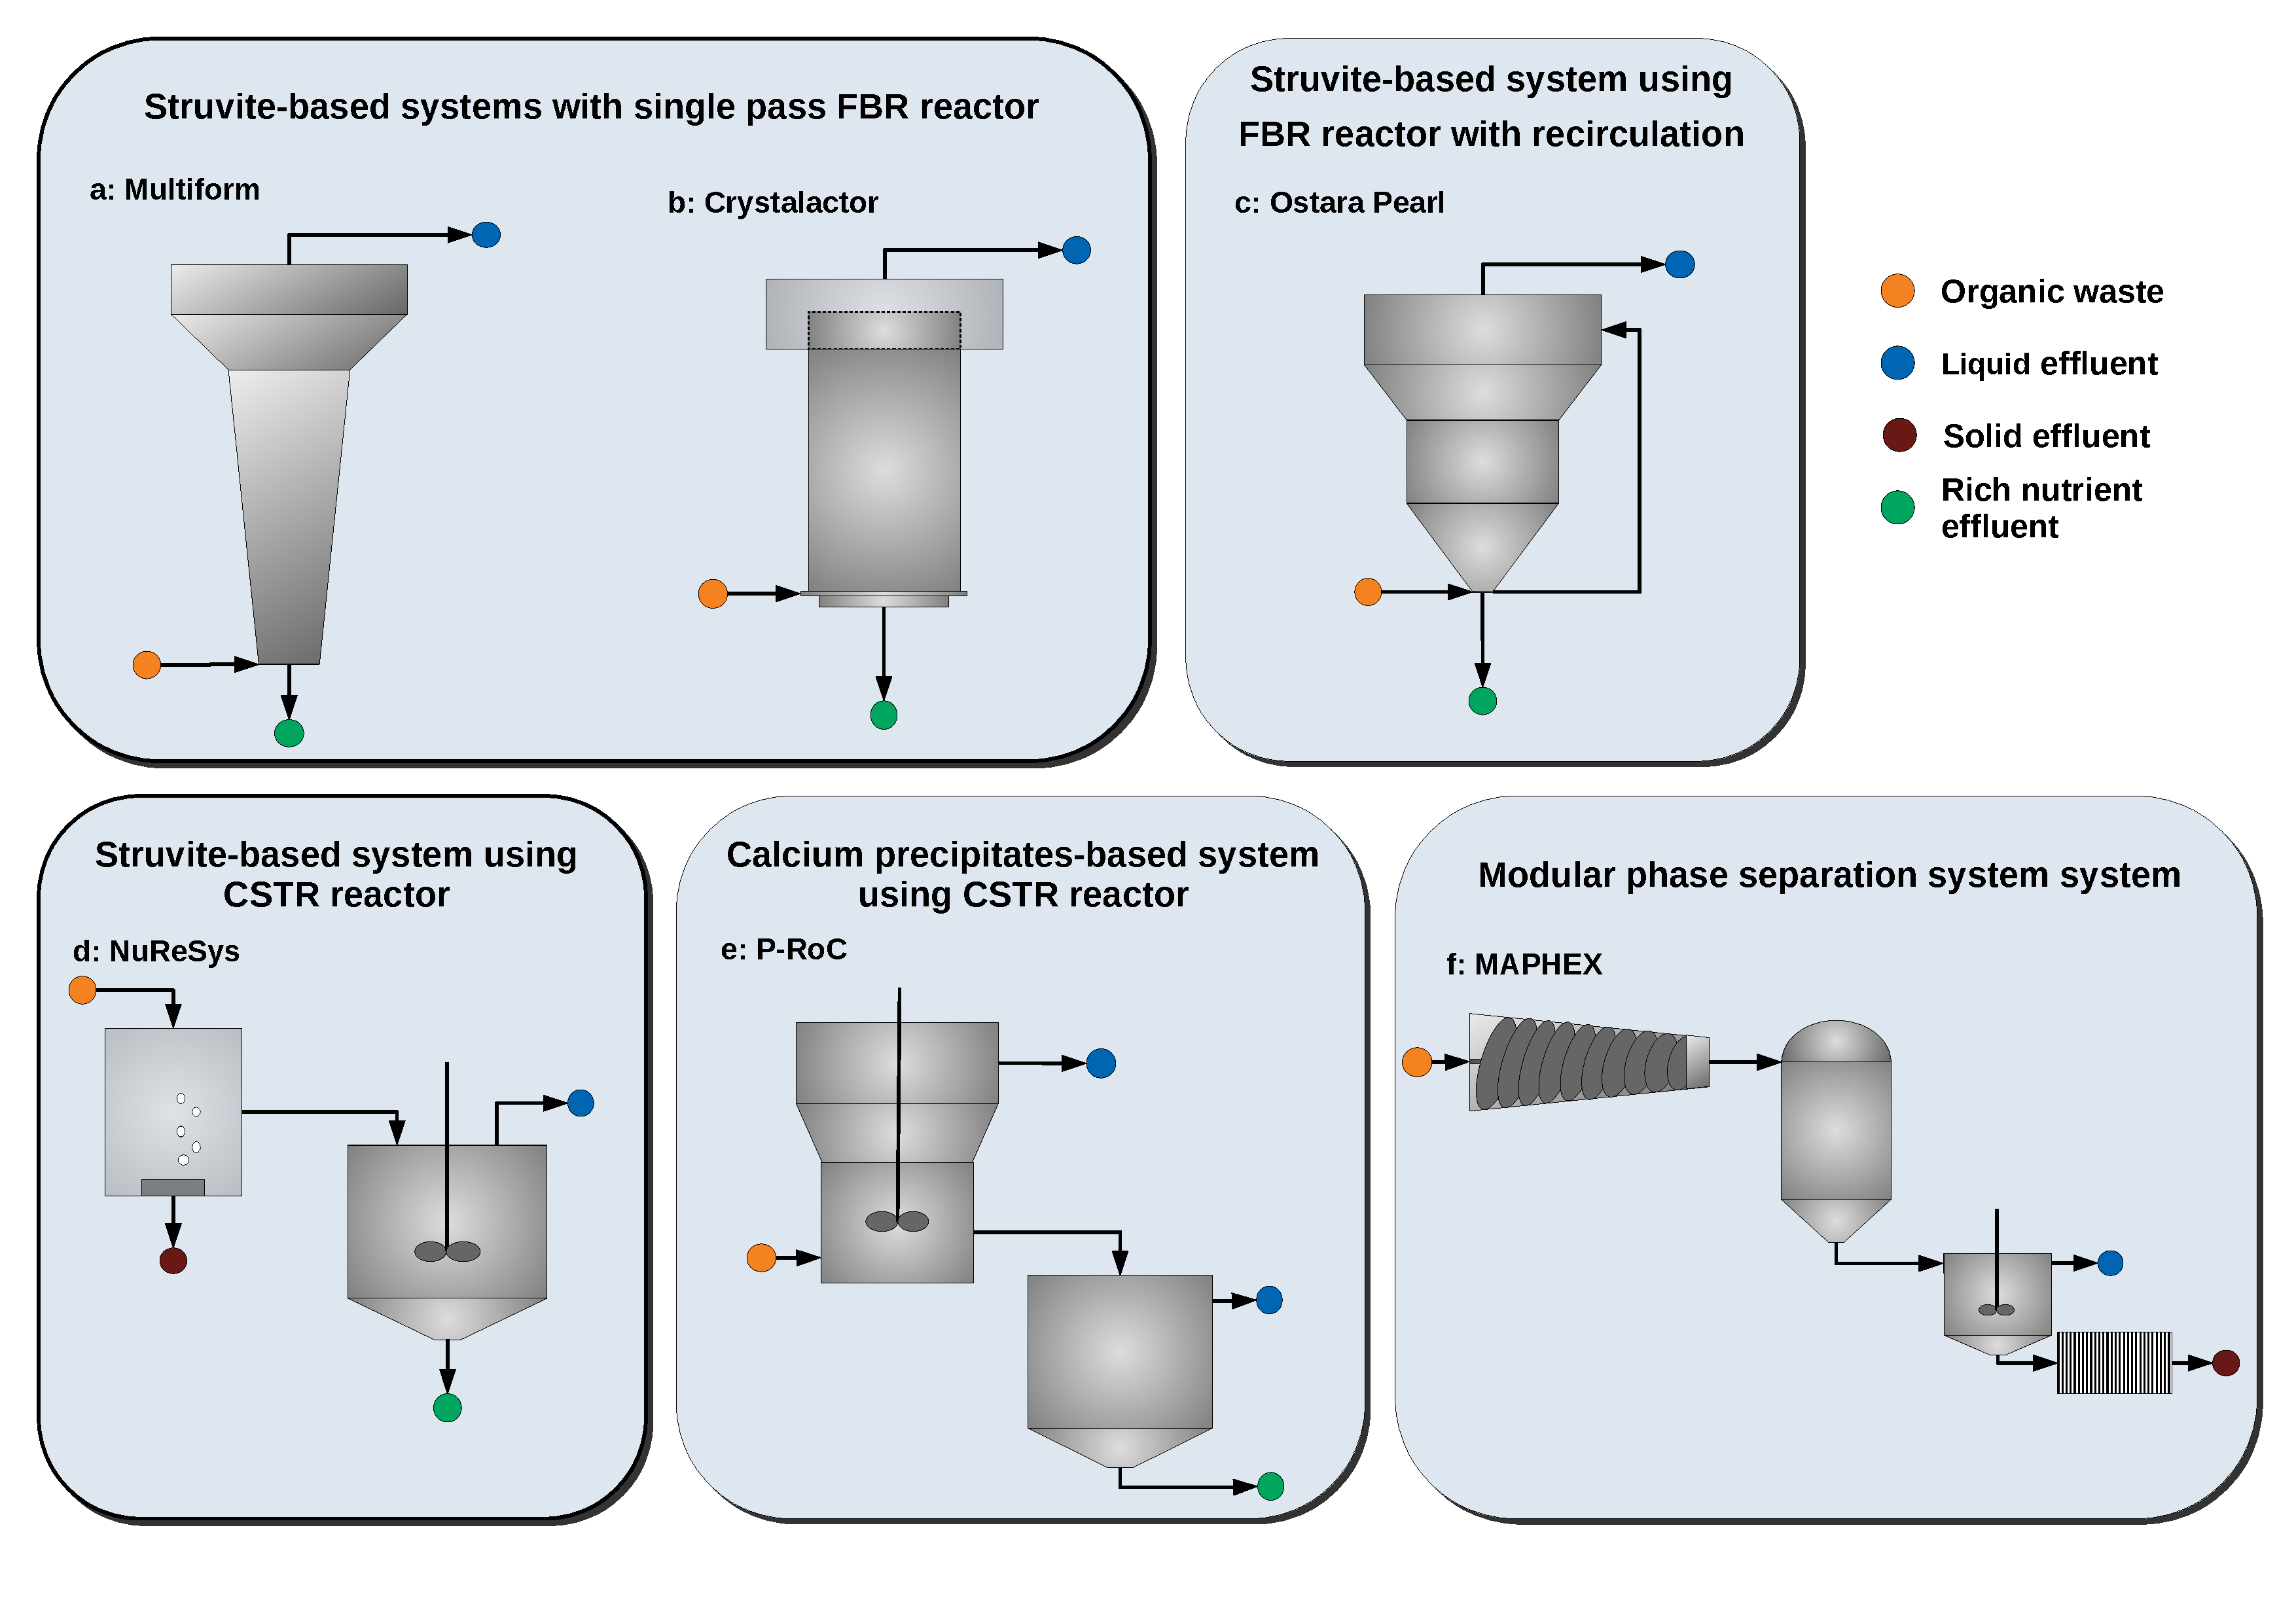
\includegraphics[width=0.85\linewidth, trim={0cm 2.5cm 0cm 0cm},clip]{diagrams.pdf} 
%	\caption{Flowsheets of the nutrient recovery systems considered in the proposed framework. a: Multiform, b: Crystalactor, c: Ostara Pearl, d: Nuresys, e: P-RoC, f: MAPHEX.}
%	\label{fig:techs_diagrams}
%\end{figure}


%\paragraph{Phosphorus recovery as struvite in single pass FBR reactor: Multiform Harvest and Crystalactor.}
%Phosphorus can be recovered in the form of struvite using single pass fluidized bed reactors (FBR). Multiform Harvest and Crystalactor are commercial technologies using this configuration, based on single pass fluidized bed reactors, with no recirculation and conical or cylindrical design respectively, where the organic waste is pumped, carrying out the struvite formation. The struvite particles grow, increasing their size, until their mass overcome the drag force of the uplift stream.
%
%Multiform, Figure \ref{fig:techs_diagrams}a, is a nutrient recovery system developed by the U.S. based company Multiform Harvest. It is a struvite-based process designed to be simple, robust, and fully automatized. Large struvite particles settle towards the reactor base, from where they are removed to be dried before obtaining the final product. MgCl\textsubscript{2} is supplied to the reactor for increasing struvite supersaturation, enhancing its precipitation. pH is adjusted using sodium hydroxide. The conical design of the reactor keeps the small and lighter particles on the large diameter section at the top of the reactor, where the superficial velocity is slower. As the particles increase their mass, they settle gradually to lower levels of the reactor, where the diameter is smaller and the superficial velocity and drag force larger, until they are finally settled on the bottom of the reactor. The liquid phase exits the reactor from the top, where the cross-section is the widest, to ensure the retention of struvite fines \citep{Pearl2Kcost2}.
%The techno-economic model for the Multiform process considers a unique size able to process up to 38.5 kg of phosphorus (P-PO\textsubscript{4}) per day, with an associated capital cost of 625,000 USD per each Multiform unit, plus 420,000 USD for the struvite dryer that serves all Multiform units. The operating cost for the Multiform system unit is 15.419 USD per kg of P-PO\textsubscript{4} processed \citep{Pearl2Kcost2}.
%
%Crystalactor is a nutrient recovery system created by the Dutch company Royal HaskoningDHV, Figure \ref{fig:techs_diagrams}b. It is based on a fluidized bed reactor where phosphorus is recovered as precipitates. It can be configured to recover phosphate in the form of calcium phosphates or struvite, depending on the reactant supplied. The model included in the tool considers that the system is configured for struvite production since struvite has a more consolidated market than calcium precipitates to sell the final product recovered. Under this configuration, the reactor is filled with small struvite particles playing the role of seeds to promote the precipitation process, and MgCl\textsubscript{2} is supplied to increase struvite supersaturation \citep{egle_phosphorus_2016}.
%It is considered that each unit is able to process up to 137.7 kg of P-PO\textsubscript{4} per day. The economy of scale for Crystalactor costs can be captured through the previous work developed by \citet{egle_phosphorus_2016} using Eq. \ref{eq:capital_cost_crystalactor}, where $n_{\text{Crystalactor}}$ represents the number of Crystalactor units installed. Crystalactor operating cost assumed is 2.12 USD per kg of P-PO\textsubscript{4} processed \citep{egle_phosphorus_2016}.
%
%\begin{align}
%& \text{Capital cost}_{\text{Crystalactor}}= 2.3 \cdot 10^{6} + 714,285.71 \cdot n_{\text{Crystalactor}} \label{eq:capital_cost_crystalactor}
%\end{align}
%
%\paragraph{Phosphorus recovery as struvite in a FBR reactor with recirculation: Ostara Pearl.}
%Pearl is a struvite-based nutrient recovery system developed by the Canadian company Ostara, Figure \ref{fig:techs_diagrams}c. The system is based on a continuous operated fluized bed reactor (FBR) reactor where the waste stream is in contact with struvite particles, which promotes the precipitation of struvite. To increase the supersaturation of struvite and enhance its precipitation, MgCl\textsubscript{2} is supplied to the reactor in a molar ratio of 2 mol of Mg per mol of phosphate. pH is adjusted using sodium hydroxide. In the reactor, the struvite particles grow until they reach a critical mass enough to overcome the drag force of the uplift liquid. To achieve different superficial velocities along the reactor, the diameter of the reactor increases with the height, providing sufficient superficial velocity in the bottom of the vessel to fluidize the struvite seeds, while the larger diameter in the top of the reactor reduces the liquid uplift velocity, allowing retention of fine crystal seed particles in the reactor. Large struvite particles sink towards the base of the reactor, from where they are periodically withdrawn. To increase the liquid flow in the reactor and achieve larger superficial velocities, an internal recirculation loop is used to recirculate liquid to the bottom of the reactor. A drying step is performed to remove the excess of moisture contained in the struvite particles obtained from the reactor.  The liquid stream leaves the reactor at the top, where the cross-section has the largest diameter to ensure the retention of struvite fines. The fraction of phosphorus recovered as struvite is estimated using Eq. \ref{eq:sigmoidal_Ca_StrYield}, since the amount of phosphorus recovered is a function of the calcium present in the organic waste stream.
%
%Based on the information reported by Ostara \citep{Pearl2Kcost2}, standard equipment sizes for the Pearl system are divided in three different capacities, Pearl 500, Pearl 2K, and Pearl 10K, with a load capacities range from 65 to 1250 kg PO\textsubscript{4} per day, as shown in Table \ref{table:ostara_costs}. Investment and operating costs for the Ostara Pearl process, including the cost of the conveyor dryer included in the process, can be found in Table \ref{table:ostara_costs} \citep{Pearl500cost1, Pearl2Kcost1, Pearl2Kcost2, Pearl10Kcost1}. A investment cost-equipment cost ratio of 1.9 has been considered \citep{Pearl2Kcost2}.
%
%\begin{table}[H] 
%	\begin{adjustwidth}{}{}
%		\centering
%		\caption{Sizing and equipment cost estimated for Ostara Pearl process} \label{table:ostara_costs}
%		\begin{tabular}{c c c c}
%			\toprule
%			& Pearl 500 & Pearl 2K	& Pearl 10K	\\ \midrule
%			%			\cmidrule(lr){2-4}
%			Load capacity $\left(\frac{\text{kg}_{\text{P-PO}_\text{4}}}{day}\right)$ & 65 & 250 & 1250 	\\
%			Capital cost (USD)	& $2.3 \cdot 10^{6}$ & $3.1 \cdot 10^{6}$  & $10.0 \cdot 10^{6}$  	\\
%			$\frac{\text{Investment}}{  \frac{\text{kg}_{\text{PO}_\text{4}}}{\text{day}}}$  $\left(\frac{USD}{kg}\right)$	& 35,385 & 12,252 & 8,000  \\ 
%			\bottomrule 
%		\end{tabular}
%	\end{adjustwidth}
%\end{table}
%
%\paragraph{Phosphorus recovery as struvite in a CSTR reactor: NuReSys.}
%NuReSys, Figure \ref{fig:techs_diagrams}d is a nutrient recovery technology develop in Belgium by Nutrients Recovery Systems. Struvite formation is carried out in a continuous stirred tank reactor (CSTR), equipped with a special impeller to minimize the breakage of struvite crystals. NuReSys process uses a stripper as pretreatment where air is injected in the organic waste, decomposing organic carbon and increasing the pH. If pH adjustment is needed, sodium hydroxide is added to the CSTR vessel. The liquid stream is fed into the CSTR reactor for struvite precipitation. Similar to other struvite-based processes, MgCl\textsubscript{2} is supplied to the reactor to increase struvite supersaturation. After struvite precipitation, both solid and liquid phases are extracted from the reactor in the same stream and it is injected in a settler where the separation of phases is carried out. Struvite fines are separated from the largest struvite particles through a hydrocyclone and they are recirculate to the process. The struvite particles are dried before their final collection \citep{Pearl2Kcost2}.
%
%Considering the data available, it has been assumed that each NuReSys system unit is able to process up to 204 kg of P-PO\textsubscript{4} per day, with an associated capital cost of 1,380,655 USD. NuReSys operating cost is 6.22 USD per kg of P-PO\textsubscript{4} processed \citep{Pearl2Kcost2}.
%
%\paragraph{Phosphorus recovery as calcium precipitates in CSTR a reactor: P-RoC.}
%P-RoC is a patented system by the Karlsruhe Institute of Technology (Germany) for phosphorus recovering as calcium precipitates, Figure \ref{fig:techs_diagrams}e. P-RoC is based on a reactive substrate, calcium-silicate hydrate (CSH), which is the support on which phosphorus is deposited forming a calcium precipitate. The process is carried out in a CSTR reactor, where the precipitates are formed. Liquid and solid phases are separated by sedimentation in a settler, and the obtained particles are finally dried in two consecutive steps composed by a belt filter and a conveyor dryer \citep{ehbrecht_p-recovery_2011, ehbrecht_p-roc-technology_nodate}.
%
%As P-RoC is not yet a fully commercial technology, the capital cost is estimated through a preliminary design of each equipment: CSTR reactor, settler, and belt dryer. The estimation of the investment of the CSTR reactor unit is the result of the sum of the vessel and the agitator costs. For design purposes, a maximum CSTR volume of 45 m\textsuperscript{3} is considered \citep{CAPCOST}. For larger volumes, multiple units installed in parallel are considered, computed through in Eq. 1 of the Supplementary Material. The vessel cost is based on data reported by CAPCOST \citep{CAPCOST}, from which the correlation shown in Fig 5 of the Supplementary Material has been developed.
%
%The clarifier cost has been estimated as a vessel, using the correlation shown in Figure 5 of the Supplementary Material. The residence time assumed is 1 hour \citep{ehbrecht_p-recovery_2011}. A vacuum conveyor filter has been selected for struvite recovery from the outlet reactor stream since previous studies report the use of this equipment \citep{Matynia}. For design purposes, a filter rate of 0.011 kg/(m\textsuperscript{2}·s) and a maximum area of 1,200 ft\textsuperscript{2} are considered \citep{Walas}. The unit cost is based on the correlations reported in \citet{Walas}. This correlation is based on the area of the filter. Vacuum conveyor filter area and cost are collected in Eqs. 2 and 3 of the Supplementary Material. The final drying of struvite is achieved with a conveyor dryer. For design purposes, a drying time of 2,100 s and a dryer capacity of 20.85 kg/m\textsuperscript{2} are assumed based on data reported on Table 12-21 of \citet{Perry}. 
%The cost estimation for a conveyor unit is based on data reported in Table 12-23 of \citet{Perry}. The correlation developed, relating the unit cost and its area can be found in Figure 6 of the Supplementary Material. Additionally, based on these data, a maximum conveyor dryer size of 90 m\textsuperscript{2} is assumed.
%
%Based on data reported by \citet{egle_phosphorus_2016}, it has been considered that operating costs are variable as a function of the processed amount of P-PO\textsubscript{4}.
%Dryer loading, area and cost are estimated using Eqs. 4 to 6 of the Supplementary Material.
%
%\paragraph{Phosphorus recovery through a modular phases separation system: MAPHEX.}
%MAPHEX is a nutrient recovery system based on physico-chemical separations developed by Penn State University and the USDA, Figure \ref{fig:techs_diagrams}f. It involves three stages: liquid-solid separation with an screw press and a centrifuge, addition of iron sulfate to improve nutrients retention, and filtration with diatomaceous earth as filter media. It is conceived as a mobile modular system which can be set in two interconnected truck trailers \citep{church_novel_2016, church_versatility_2018}.
%Each MAPHEX unit is able to process up to 18.54 kg of P-PO\textsubscript{4} fed per day, with an associated operating cost of 110.8 USD per kg of P-PO\textsubscript{4} processed. Capital cost of a MAPHEX unit is 291,000 USD \citep{church_novel_2016, church_versatility_2018}.

\subsubsection{Incentives for the installation of nutrient recovery systems}
COW2NUTRIENT can evaluate the effect of different kinds of incentives on the economic performance of the nutrient recovery systems. These incentives can be received as a result of the recovery of phosphorus, in the form of P-credits, or for the generation of electricity or biomethane, in form of Renewable Energy Certificates (REC) and Renewable Identification Numbers (RIN) respectively. Renewable Energy Credits are a mechanism implemented in the US which guarantees that energy is generated from renewable sources, providing a system for trading produced renewable electricity. Each produced renewable megawatt-hour generates one REC, that can be sold separately from the electricity commodity itself and can be used to meet regulatory requirements by generators, trades, or end-users. On the other hand, RINs are identification numbers assigned to batches of biofuel, allowing their tracking through the production, purchase, and final usage. The allocation of RINs is associated with the allocation of incentives for the generation bio-fuels. 
%In addition, potential incentives to partially cover the capital cost of the nutrient recover process are considered.
The considered values for the different incentives are listed in Table 4S of the Supplementary Material.

\subsection{Multi-criteria decision model}
The determination of the most suitable nutrient management process is not a trivial procedure since multiple criteria play a critical role at the decision-making stage. COW2NUTRIENT performs the selection of P recovery technologies considering information concerning environmental, economic, and technology readiness dimensions. The integration of these dimensions is justified by the need to find the most suitable system for each CAFO by balancing operating cost and efficiency in the mitigation of nutrient pollution according to the local environmental vulnerability to eutrophication. Finally, the technical maturity of each system is also considered to assess the development level of the different processes. Therefore, a multi-criteria decision analysis (MCDA) model was developed to address the selection of the most suitable phosphorus recovery systems for each studied CAFO. The workflow of the MCDA model is summarized in Figure \ref{fig:MCDA_SMAA}.

\begin{figure}[h]
	\centering
	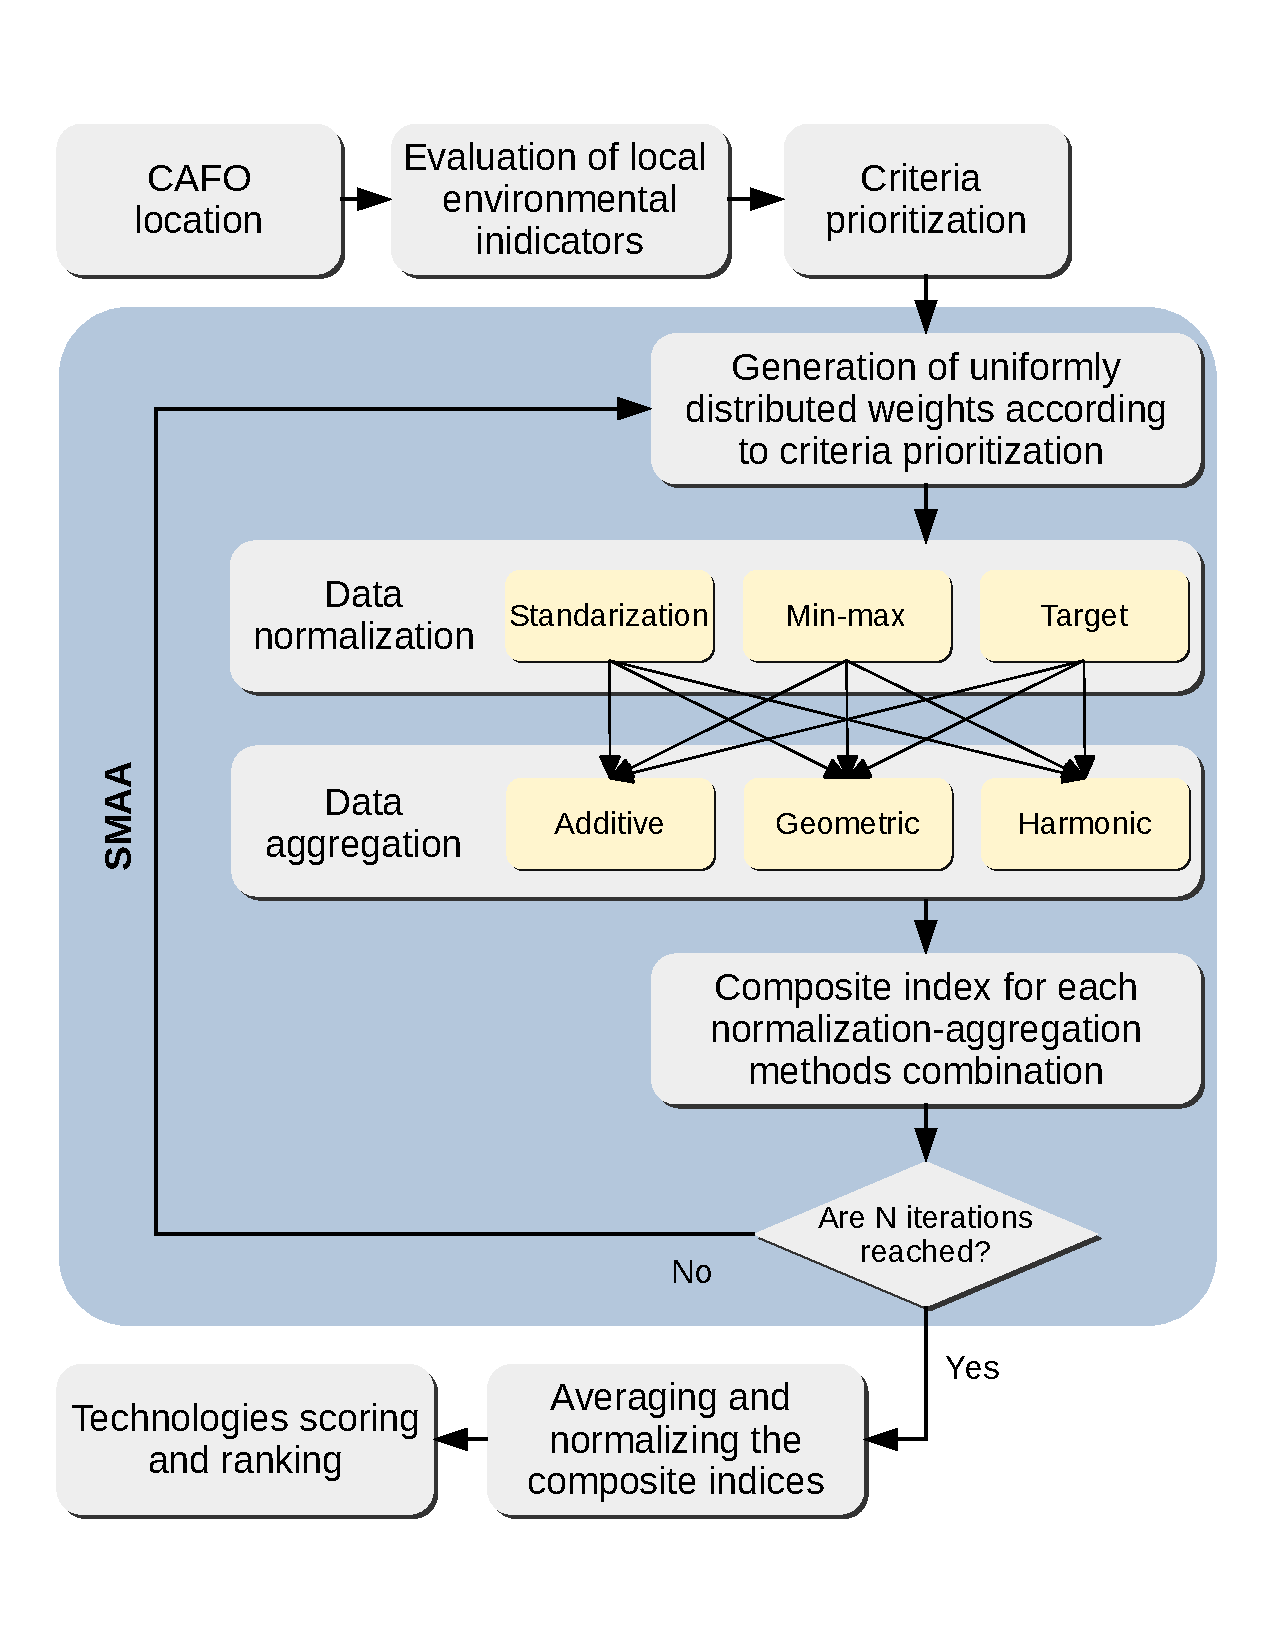
\includegraphics[width=0.6\linewidth, trim={0cm 1cm 0cm 1cm},clip]{MCDA_SMAA.pdf} 
	\caption{Flowsheet for the MCDA model.}
	\label{fig:MCDA_SMAA}
\end{figure}

Five criteria are combined in a composite index for the assessment of the environmental, economic, and technology maturity dimensions of the different technologies. Two environmental criteria are studied to assess the performance of the different technologies to mitigate phosphorus releases from CAFOs, i.e., the fraction of phosphorus recovered, and the potential environmental threat for the local ecosystem of the effluents containing the non-recovered phosphorus evaluated through the eutrophication potential of the effluents. The economic aspect is considered by means of two criteria, the economic barrier for the implementation of P recovery processes, measured in terms of capital cost, and the overall economic performance of the systems, which is evaluated through the net present value (NPV) \citep{sinnott2014chemical}. Finally, the technological maturity of the different technologies is considered though the technology readiness level (TRL) index. The construction of a composite index integrating these criteria is composed of three steps: criteria normalization, weighting, and aggregation \citep{MarcoCinelli2020}.
%These five criteria are weighted according to their importance and combined in a composite index that characterizes each nutrient recovery system in order to compare the different technologies.
%Indices are an intuitive approach for the stakeholders since they allow summarizing the information of the different indicators considered in one parameter and rank the technologies according to their performance, identifying the best process with respect to the others \cite{MarcoCinelli2020}.

%TRL index is set as the criteria with highest preference since the aim of the tool is to provide phosphorus recovery processes feasible to be installed and operated in livestock facilities. The prioritization of environmental and economic criteria is carried out based on the environmental information the location of the CAFO evaluated. If there is immediate environmental risk by nutrient pollution (high values for TSI or soil fertility), the environmental performance has preference over economic performance. If there is environmental risk in the long term due to the unbalance between anthropogenic phosphorus releases and uptakes (negative value of TES indicator), or there is no environmental risk, the economic performance has preference over the environmental performance. If there is no data for any criterion in the studied region, this criterion is exempt from the evaluation procedure. Table \ref{table:criteria_preference} shows in detail the criteria preference in function of environmental geographic indicators for nutrient pollution. Optionally, users can disable the criteria prioritization based on environmental geographic information and set customized weights for the criteria to adapt the tool to different decision-making scenarios.

\begin{table}[]
	\centering
	\caption{Criteria preference as a function of the GIS-based environmental indicators for nutrient pollution.} \label{table:criteria_preference}
	\begin{threeparttable}
		\begin{tabular}{@{}ccc@{}}
			\toprule
			\begin{tabular}[c]{@{}c@{}}Local environmental \\ indicators values\end{tabular}                                                                                              & Criteria ranking                                                                                                                                          & Description                                                                                                                                                                    \\ \midrule \\
			\begin{tabular}[c]{@{}c@{}}Condition 1:\\ TES $>$ TSI and \\ TES $>$ Soil fertility\\ \\ Condition 2:\\ TES = Unbalanced\end{tabular}                        & \begin{tabular}[c]{@{}c@{}}TRL $>$ NPV $>$ \\ Capital cost $>$ TP recovered $>$ \\ Eutrophication potential\end{tabular}  & \begin{tabular}[c]{@{}c@{}}Unbalanced phosphorus releases \\ but no immediate threat to \\ soil and water bodies. \\ \\ Prevalence of economic criteria for \\ nutrient recovery system selection.\end{tabular} \\ \\ \midrule \\
			\begin{tabular}[c]{@{}c@{}}Condition 1:\\ TSI $\geq$ TES or\\ TSI $\geq$ Soil fertility\\ \\ Condition 2:\\ TSI = Eutrophic or\\ Hypereutrophic\end{tabular}    & \begin{tabular}[c]{@{}c@{}}TRL $>$ \\ Eutrophication potential $>$ NPV $>$ \\ TP recovered $>$ Capital cost\end{tabular} & \begin{tabular}[c]{@{}c@{}}High Trophic State Index. \\ \\ Inmmediate environmental risk \\ due to potential algal blooms. \\ \\ Prevalence of environmental criteria \\ for nutrient recovery system selection.\end{tabular}    \\  \\ \\ \midrule \\
			\begin{tabular}[c]{@{}c@{}}Condition 1:\\ Soil fertility $\geq$ TES and \\ Soil fertility $>$ TSI \\ \\ Condition 2:\\ Soil fertility = Excessive\end{tabular} & \begin{tabular}[c]{@{}c@{}}TRL $>$ TP recovered $>$ \\ NPV $>$ Eutrophication potential $>$ \\ Capital cost\end{tabular}  & \begin{tabular}[c]{@{}c@{}}Excessive P in soil. \\ \\ Inmmediate environmental risk \\ due to potential P runoff. \\ \\ Prevalence of environmental criteria \\ for nutrient recovery system selection.\end{tabular}           \\    \\ \\ \midrule \\
			\multicolumn{1}{l}{\begin{tabular}[c]{@{}c@{}}Condition:\\ TES $\neq$ Saturated\\ and \\ TSI $\neq$ Eutrophic or\\ Hypereutrophic\\ and\\ Soil fertility $\neq$ Excessive\end{tabular}}      & \begin{tabular}[c]{@{}c@{}}TRL $>$ NPV $>$ \\ Capital cost $>$ TP recovered $>$ \\ Eutrophication potential\end{tabular}  & \multicolumn{1}{c}{\begin{tabular}[c]{@{}c@{}}No environmental risk.\\ \\ Prevalence of economic criteria for\\ nutrient recovery system selection.\end{tabular}}                                                     \\  \\ \bottomrule
		\end{tabular}
		\begin{tablenotes}
			\item TRL: Technology Readiness Level
			\item TSI: Trophic State Index
			\item TES: Techno-Ecological Synergy sustainability metric
			\item NPV: Net Present Value
			\item TP: Total Phosphorus
		\end{tablenotes}
	\end{threeparttable}
\end{table}

\subsubsection{Data normalization}
Since each criteria has a different range of potential values, they must be normalized to a common scale to allow each criteria to be compared with the others. However, the composite index 
%can be biased by the methodology used to construct the index. 
can be affected by the normalization technique used. In order to study the robustness of the composite index obtained, and to address the uncertainty originated by data normalization, normalized data using standardization, min-max, and target normalization methods is calculated
%To address this issue, different normalization techniques are evaluated in order to systematically assess the stability of the scores obtained and the ranking robustness
%of the ranking
%of the phosphorus recovery technologies. Among the normalization techniques, linear normalization methods have been considered, i.e. standardization, min-max, and target methods
\citep{HandbookCompositeIndicators}.

\subsubsection{Criteria weighting}
The normalized criteria are weighted to set the relative importance of each criterion, prioritizing some criteria over others. This is needed in order to 
%one of the main objectives of the COW2NUTRIENT framework is to adapt the selection of P recovery technologies to the environmental vulnerability to eutrophication of each region, balancing the operating cost of the systems, and the P recovery efficiency. As a result, we 
obtain a flexible decision method able to balance the operating cost of the systems and the P recovery efficiency as a function of the environmental vulnerability to eutrophication of each region. The minimization of the operating costs is prioritized in regions with low eutrophication risk, while the efficiency of P recovery is more relevant in regions affected by nutrient pollution. Therefore, 
%Since the weighting of criteria have significant effect on the multicomposite index obtained. 
the criteria are dynamically weighted according to the values of TSI, TES and Mehlich 3 phosphorus concentration in each region studied. The preference of criteria as a function of the environmental vulnerability to eutrophication is shown in Table \ref{table:criteria_preference}.
% shows in detail the criteria preference in function of environmental geographic indicators for nutrient pollution
%local vulnerability to nutrient pollution.
%five criteria are weighted according to their importance and combined in a composite index that characterizes each nutrient recovery system in order to compare the different technologies. 
%
%Since the objective of this framework is to select nutrient management systems that are feasible to install and operate at livestock facilities, the TRL index is set as the criteria with highest preference. 
%
%The prioritization of environmental and economic criteria is carried out based on the information about the environmental vulnerability to nutrient pollution in the watershed where the CAFO under evaluation is located. 
On the one hand, if there is immediate environmental risk by nutrient pollution (i.e., high values for TSI or soil fertility),
%the environmental performance has preference
phosphorus recovery efficiency is prioritized over economic performance. Conversely, if there is environmental risk in the long run due to the unbalance between anthropogenic phosphorus releases and uptakes (negative value of TES indicator), or there is no potential environmental risk, the economic performance 
%has preference 
is prioritized over the
%environmental performance
phosphorus recovery efficiency. 
Finally, since the objective of this framework is to select P recovery systems that are feasible to install and operate in CAFOs, the TRL index is set as the criteria with highest preference in all cases in order to minimize the risk of selecting non-full-scale processes. As a result, the selection of processes with low TRL will be hampered unless they have good economic or environmental performance.
%If there is no data for any criterion in the studied region, this criterion is exempt from the evaluation procedure. 


The procedure described above sets the prioritization of criteria, i.e., they can be sorted in order of importance. However, it does not provide an specific value for the weights, which values are unknown. In order to avoid the risk of biasing the decision-making procedure setting arbitrary values for the weights, a stochastic multi-criteria acceptability analysis (SMAA) is used to explore the weights space \citep{tervonen_implementing_2007}. Through this approach, the feasible space of each weight (i.e., the space delimited by the previous and the subsequent weights) is explored through the Monte Carlo method, retrieving a set of weights for all criteria according to the assigned order. The SMAA is formulated by defining the set of $n$ weights ($\omega$) as a non-negative set which elements must sum 1, as shown in Eqs. \ref{eq:weight_def_1} and \ref{eq:weight_def_2}.

\begin{align}
	& \omega_{j} \geq 0 \ \forall \ j \ \in \ {n} \label{eq:weight_def_1}\\
	& \sum_{j=1}^{n} \omega_{j} = 1  \label{eq:weight_def_2} \\
%\end{align}
%
%\begin{align}
	& \omega_{j1} \geq \omega_{j2} \geq ... \geq \omega_{jn} \label{eq:weight_def_3}
\end{align}

The preference information of the criteria, defined through the ranking of the criteria shown in Table \ref{table:criteria_preference}, is expressed as a sequence of inequality constraints, Eq. \ref{eq:weight_def_3}. A detailed description of the SMAA method can be found in \citet{tervonen_implementing_2007}. A number of Monte-Carlo simulations $\left(N\right)$ of 100 is assumed as a trade-off between computational cost and MCDA model performance.
%Optionally, in order to evaluate alternative approaches other than the vulnerability to nutrient pollution, the framework allows for setting customized criteria weights.

\subsubsection{Criteria aggregation}
%Finally, 
The aggregation stage merges the weighted criteria, resulting in the composite index. 
%However, the value of a composite index can be biased by the methodology used to construct the index. To address this issue, different normalization and aggregation techniques are evaluated in order to systematically assess the stability of the indexes obtained and the robustness of the ranking of nutrient recovery technologies. 
%The use of different normalization methods allows the evaluation of different approaches for the comparison of the environmental indicators.
Similarly to the normalization stage, different aggregation methods are evaluated to improve the robustness of the solutions retrieved by the framework. Different aggregation schemes denote different degrees of compensability between indicators, i.e. a deficit in one criteria can be fully, partially, or not compensated by a surplus in other criteria \citep{MarcoCinelli2020}. Three aggregation functions are evaluated including full compensation (additive aggregation) and partial compensation schemes (geometric and harmonic aggregation methods). Nine composite indexes are obtained for each P recovery technology combining normalization and aggregation techniques, as shown in Figure \ref{fig:MCDA_SMAA}.
%A composite index of each technology for the nine combinations of normalization-aggregation functions is obtained averaging the values obtained in the SMAA. 
Finally, the composites indexes are normalized in a range from 0 to 1 and ranked to determine the most suitable P recovery process for the CAFO under study.

%\begin{table}[]
%	\centering
%	\caption{Combinations of normalization and aggregation methods for constructing the composite indexes.} \label{table:composite_index}
%	{\color{blue}{
%	\begin{tabular}{@{}ccc@{}}
%		\toprule
%		Composite index (CI) & Normalization method & Aggregation method \\ \midrule
%		CI 1                 & Standardization      & Additive           \\
%		CI 2                 & Min-max              & Additive           \\
%		CI 3                 & Target               & Additive           \\
%		CI 4                 & Standardization      & Geometric          \\
%		CI 5                 & Min-max              & Geometric          \\
%		CI 6                 & Target               & Geometric          \\
%		CI 7                 & Standardization      & Harmonic           \\
%		CI 8                 & Min-max              & Harmonic           \\
%		CI 9                 & Target               & Harmonic           \\ \bottomrule
%	\end{tabular}
%	}}
%\end{table}

%, thus obtaining the final score for each phosphorus recovery systems. Finally, the technologies are ranked based on these scores.
%Indexes for all combinations of normalization-aggregation methods are computed. 

%Since the preference of criteria is known as a function of the GIS-based environmental indicators (see Table \ref{table:criteria_preference}), but the value of the weights is unknown, a stochastic multicriteria acceptability analysis (SMAA) is used to explore the weights space. To formulate the SMAA, the set of $n$ weights ($\omega$) is defined as a non-negative set whose elements must sum 1, as shown in Eqs. \ref{eq:weight_def_1} and \ref{eq:weight_def_2}.
%
%\begin{align}
%& \omega_{j} \geq 0 \ \forall \ j \ \in \ {n} \label{eq:weight_def_1}\\
%& \sum_{j=1}^{n} \omega_{j} = 1  \label{eq:weight_def_2}
%\end{align}
%
%In addition to Eqs. \ref{eq:weight_def_1} and \ref{eq:weight_def_2}, preference information of the criteria, defined through the ranking of the criteria shown in Table \ref{table:criteria_preference}, is expressed as a sequence of inequality constraints, Eq. \ref{eq:weight_def_3}.
%
%\begin{align}
%& \omega_{j1} \geq \omega_{j2} \geq ... \geq \omega_{jn} \label{eq:weight_def_3}
%\end{align}
%
%Therefore, the feasible weight space, including preference information in the form of a ranking of criteria, is defined by the Eqs. \ref{eq:weight_def_1}, \ref{eq:weight_def_2}, and \ref{eq:weight_def_3} \citep{tervonen_implementing_2007}. Figure \ref{fig:SMAA_weights} shows the feasible weight space for a problem with three criteria. The feasible space of each weight is explored through the Monte Carlo method \citep{tervonen_implementing_2007}, retrieving a set of weights for all criteria according to the assigned order. 

%The workflow of the MCDA model is summarized in Fig \ref{fig:MCDA_SMAA}. 
%The nine combinations of normalization-aggregation methods are evaluated using the sets of weights obtained in the SMAA. 
%A composite index of each technology for the nine combinations of normalization-aggregation functions is obtained averaging the values obtained in the SMAA. Finally, the composites indexes are normalized in a range from 0 to 1, thus obtaining the final score for each phosphorus recovery systems. Finally, the technologies are ranked based on these scores.
%multiple composite indexes are analyzed to determine the average index value for each technology, and to obtain the ranking of technologies.
%, as shown in Fig \ref{fig:MCDA_SMAA}. 
%A number of Monte-Carlo simulations of 100 is assumed as a trade-off between computational cost and MCDA model performance.

%\begin{figure}[H]
%	\centering
%	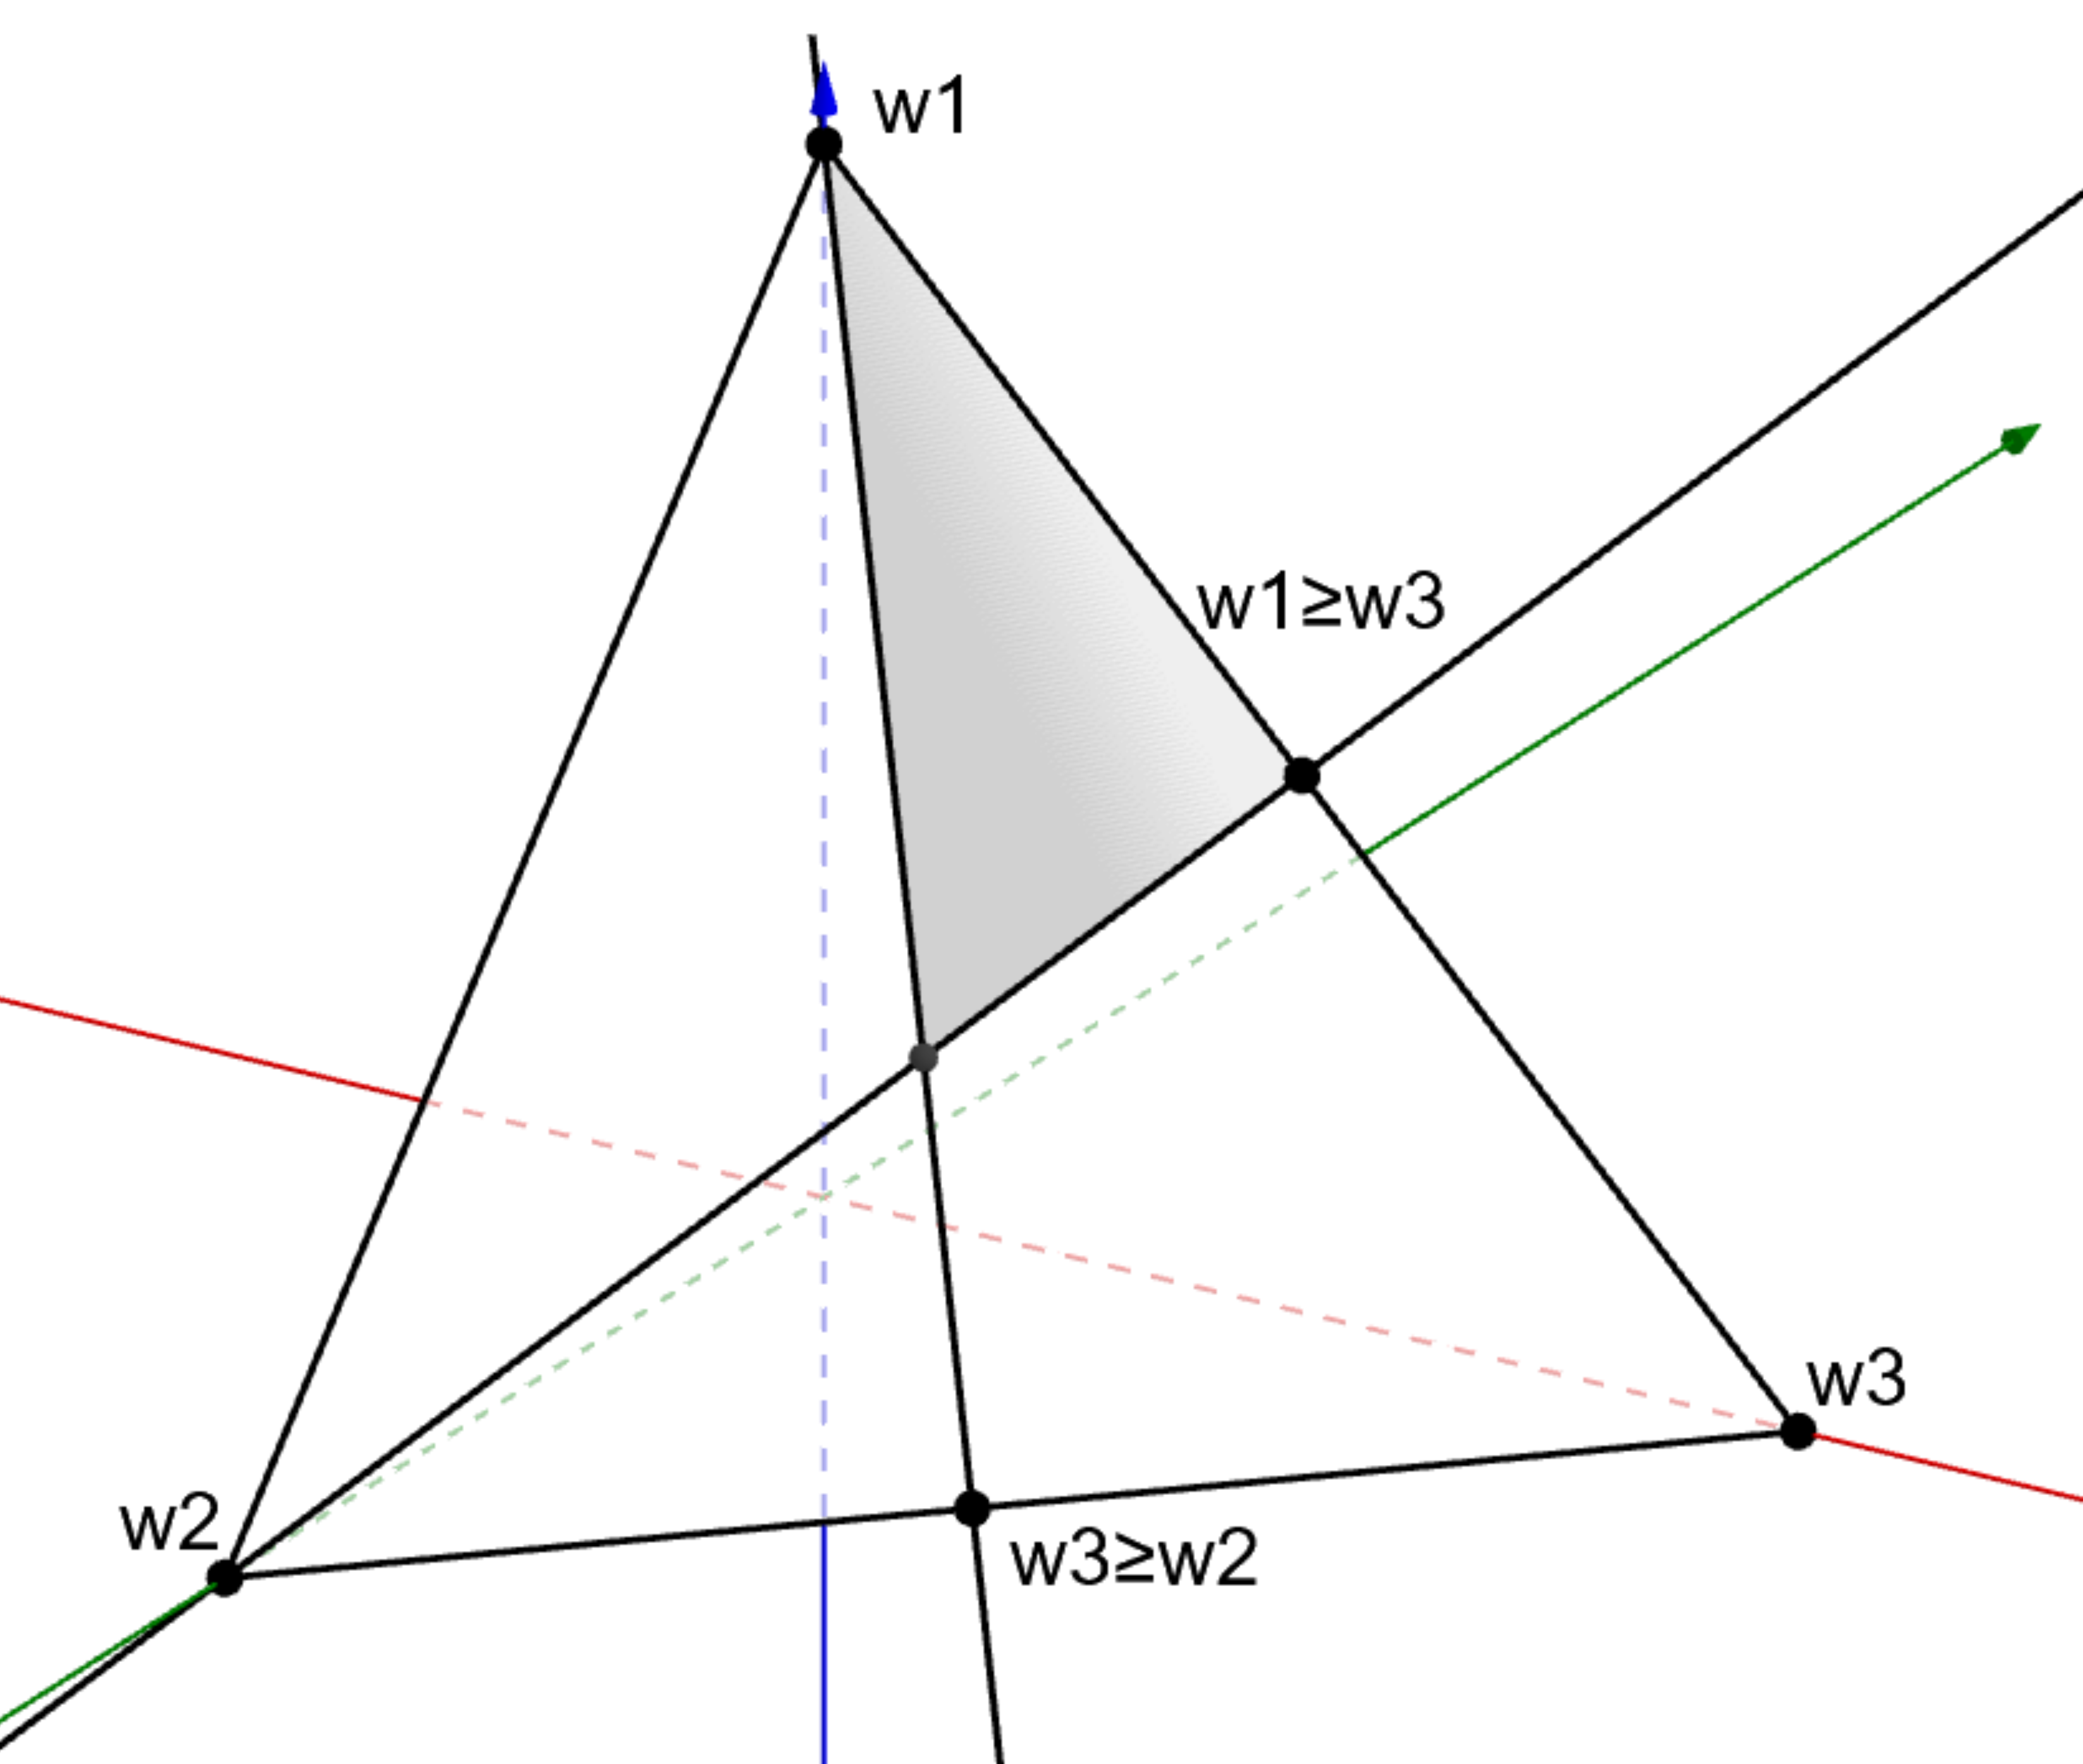
\includegraphics[width=0.4\linewidth, trim={2cm 6cm 8cm 2.5cm},clip]{SMAA.png} 
%	\caption{Example of feasible weights space for a three criteria problem considering ranking of criteria. Figure adapted from \protect\citet{tervonen_implementing_2007}}
%	\label{fig:SMAA_weights}
%\end{figure}

\subsection{Framework limitations}
The main limitations of the proposed framework lie in the uncertainty of the input data. On the one hand, since the data regarding the animal number, type of animals, and location of CAFOs are reported by the state environmental protection agencies of each state, they are considered reliable. On the other hand, to estimate the local vulnerability to phosphorus pollution throughout the contiguous US, HUC8 spatial resolution has been chosen as a trade-off solution between spatial accuracy and data uncertainty. However, more accurate results can be obtained if reliable data for phosphorus level in soils, fertilizer  application rates, etc. are available for higher spatial resolution. Particularly, further studies for developing more accurate correlations to estimate the fraction of phosphorus available to plants based on soil type and climate conditions in each region would improve the accuracy of the assessment of local risk to phosphorus pollution. Additionally, since the proposed framework is focused on phosphorus recovery for freshwater nutrient pollution prevention and control, the recovery of other resources contained in livestock manure (such as organic carbon and nitrogen) is not considered in this study.

%, for the data used to estimate the local vulnerability a trade-off solution between spatial accuracy has been , which increases at smaller scales. A HUC8 spatial resolution has been chosen as a trade-off solution between spatial accuracy and data uncertainty. However, more accurate results can be obtained if reliable data for phosphorus level in soils, fertilizer rates, etc. are available for higher spatial resolution. 


\subsection{Case study}
\subsubsection{Study region}
The Great Lakes area, located in North America, is selected in order to demonstrate the implementation of nutrient management systems at CAFOs using the COW2NUTRIENT framework. This region is selected because its high concentration of CAFO facilities, resulting in significant nutrient releases that contribute to frequent HABs and eutrophication episodes,
%that occur in this region
as well as to the nutrient legacy accumulated over time \citep{sayers2019satellite, han2012historical}. The evaluation and implementation of phosphorus recovery systems at CAFOs already in operation at the US states of Pennsylvania \citep{Pennsylvania_CAFOS}, Ohio \citep{Ohio_CAFOS}, Indiana \citep{Indiana_CAFOS}, Michigan \citep{Michigan_CAFOS}, Wisconsin \citep{Wisconsin_CAFOS}, and Minnesota \citep{Minnesota_CAFOS} are performed using the criteria prioritization based on the GIS indicators describing 
%environmental vulnerability to nutrient pollution described 
the environmental impact of nutrient pollution shown
in Table \ref{table:criteria_preference}. The states of Illinois and New York, and the Canadian province of Ontario, which are also part of the Great Lakes area, are not included due to the unavailability of reliable information about their CAFOs. A description of the studied states listing the animal units, annual manure generation, and annual phosphorus releases by the year 2019, disaggregated for dairy and beef cattle, is collected in Table 10S of the Supplementary Material. 

It should be noted that, accordingly to the US regulatory definition of CAFOs, only intensive livestock facilities with 300 animal units or more are considered in this study \citep{CAFO_definition}, resulting in the evaluation of 2,217 CAFOs. An animal unit is defined as an animal equivalent of 1,000 pounds (453.6 kg) live weight \citep{animal_unit_definition}. Animal units is used as a unit to measure the size of CAFOs due to the presence of different types of animals in the CAFOs, i.e. beef or dairy cows, and animals of different age, including heifers, calves, and adult animals. Different types of animals result in different manure generation rates and composition. Therefore, the different types of animals within each studied CAFO are normalized using the definition of animal units to estimate the amount and composition of the manure generated.

\subsubsection{Scenarios description}
Two scenarios have been evaluated, the deployment of only phosphorus recovery systems, and the integration of these processes with AD and electricity production processes. 
Incentives for the recovery of phosphorus based on the work of \citet{sampat_economic_2018} are considered, assuming a phosphorus credit value of 22 USD/kg\textsubscript{P recovered} for both scenarios. We note that this value is significantly lower than the economic impact of P release from livestock waste, valued in 74.5 USD/kg\textsubscript{P released} \citep{sampat2021valuing}. Additionally, in the scenario considering the production biogas-based electricity, a value of Renewable Energy Certificates (fixed electricity selling price) of 60 USD per MWh generated is assumed. Finally, a discount rate of 7\% is considered in both scenarios. 

\section{Results}
%\section{Results and discussion}
\subsection{Implementation of phosphorus recovery systems in the Great Lakes area}
Table \ref{table:techs_intalled} 
%{\color{blue}{Figure \ref{fig:PTechs_Distribution}}}
summarizes the results of the phosphorus recovery process selection 
%and the capital and operating costs associated with their implementation
in the Great Lakes area.
It can be observed that only three out of the six commercial processes evaluated are selected to be installed. All selected processes recover P in the form of struvite, which is a valued product that can be sold, generating income. Although the Ostara Pearl process also produces struvite, it results in larger operating costs than the technologies selected. Conversely, P-RoC recovers phosphorus in the form of calcium-based precipitates. This product lacks a well-established market, and therefore it does not generate income. In addition, P-RoC is the technology with the lowest TRL, which hampers the selection of this process. The selection of modular phosphorus recovery systems, such as MAPHEX, which due to economies of scale are especially suitable for small livestock facilities, is largely prevented by the absence of small-scale CAFOs. Therefore, a sub-set of three technologies is obtained. Therefore, it can be concluded that the selection of this pool of three technologies amongst the six systems evaluated is mainly driven by economic factors. Additionally, the low TRL of P-RoC also hampers the selection of this process.
		
The selection of the most suitable technology for each studied CAFO among the sub-set comprised by Multiform, Nuresys, and Crystalactor systems is based on the CAFO scale and local eutrophication risk, as it is discussed in the following sections.

\begin{table}[h]
	\centering
	\caption{Distribution and characteristics studied CAFOs, and phosphorus recovery processes selected. Only selected technologies are included in the table.} \label{table:techs_intalled}
	\begin{threeparttable}
		\resizebox{\columnwidth}{!}{
			\begin{tabular}{@{}ccccccccccc@{}}
				\toprule
				\multirow{3}{*}{State} & \multirow{3}{*}{\begin{tabular}[c]{@{}c@{}}CAFO\\ average size\\ (animal units)\end{tabular}} & \multirow{3}{*}{\begin{tabular}[c]{@{}c@{}}Number\\ of \\ CAFOs\end{tabular}} & \multirow{3}{*}{\begin{tabular}[c]{@{}c@{}}Manure \\ generated \\ (ton/year)\end{tabular}} & \multirow{3}{*}{\begin{tabular}[c]{@{}c@{}}P \\ recovered \\ (ton/year, (\%))\end{tabular}} & \multicolumn{6}{c}{\begin{tabular}[c]{@{}c@{}}Number of phosphorus\\ recovery systems installed\end{tabular}} \\ \cmidrule(l){6-11} 
				&                                                                                                &   &                                                                         &                                                                                       & \multicolumn{2}{c}{Multiform}       & \multicolumn{2}{c}{NuReSys}       & \multicolumn{2}{c}{Crystalactor}  \\ \cmidrule(lr){6-7} \cmidrule(lr){8-9} \cmidrule(lr){10-11}
				&                                                                                                &            &                                                                &                                                                                       & S1               & S2               & S1              & S2              & S1              & S2              \\ \midrule
				Indiana           & 1,574.41                                                                                        & 119                                                                         & $2.48 \cdot 10^6$ & 1558.8 (78.7)                            & 116               & 113               & 0               & 0               & 3               & 6               \\
				Michigan          & 2,461.52                                                                                        & 144                                                                        & $4.76 \cdot 10^6$ & 3004.4 (79.0)                                                                               & 127              & 113               & 16              & 30              & 1               & 1               \\
				Minnesota         & 634.23                                                                                        & 1,487                                                                         & $1.13 \cdot 10^7$ & 6938.1 (76.9)                                                                                & 1,477                & 1,476                & 0               & 0               & 10              & 11              \\
				Ohio              & 2,415.24                                                                                        & 53                                                                         & $1.68 \cdot 10^6$ & 1055.8   (78.6)                                                                              & 50               & 47               & 1               & 3               & 2               & 3               \\
				Pennsylvania      & 1,495.94                                                                                        & 131                                                                         & $2.59 \cdot 10^6$ & 1633.2  (78.9)                                                                              & 124               & 119               & 6               & 11              & 1               & 1               \\
				Wisconsin         & 2,628.19                                                                                        & 283                                                                        & $1.02 \cdot 10^7$ & 6510.5 (79.4)                                                                               & 262              & 255              & 6               & 7              & 15              & 21              \\ \bottomrule
		\end{tabular}}
		\begin{tablenotes}
			\item S1: Phosphorus recovery systems only.
			\item S2: Phosphorus recovery systems coupled with AD and electricity production.
		\end{tablenotes}
	\end{threeparttable}
\end{table}
		
\subsubsection{Effect of CAFOs scale on selecting P recovery systems}
%By comparing Figures \ref{fig:PTechs_Distribution_NoAD} and \ref{fig:PTechs_Distribution_AD}
%%, which illustrate the selection of technologies for both of scenarios assessed, 
%it can be observed that the integration of AD and electricity generation stages promotes the selection of {\color{blue} {processes that require larger investment costs, such as}} NuReSys and Crystalactor technologies. 
%{\color{blue}{This is because the capital costs of biogas production and upgrading processes are significantly larger than the capital costs of P recovery technologies, as it can be observed in Table \ref{table:economic_results}. Therefore, the differences of capital expenses among different phosphorus recovery technologies are blurred into the costs of the whole system (i.e., biogas production and upgrading, and P recovery processes).}}
%%Therefore, {\color{blue} {the effect of the economies of scale is increased by the integration of AD processes with phosphorus recovery processes}} as a result of.
%%Since the integration of these stages involves large capital costs, the differences of capital expenses among different phosphorus recovery technologies are blurred into the costs of the whole process, as shown in Figure \ref{fig:Capital_TechSelected}.  
%As a result, a larger number of NuReSys and Crystalactor processes are selected because of their lower operating costs, as shown in Figure \ref{fig:OPEX_TechSelected}. Additionally, the relationship between the processes selected and size of CAFOs (number of animal units) described previously can be observed in Figure \ref{fig:Capital_TechSelected}. 

%Multiform is the predominant phosphorus recovery process in all the studied states.
A relationship between CAFOs size and the selected technologies can be observed in Table \ref{table:techs_intalled}.
%Additionally, the technologies selected in the scenario considering anaerobic digestion are different than those selected if only the implementation of phosphorus recovery systems is considered, 
This relationship is also observed in Figures \ref{fig:PTechs_Distribution} and \ref{fig:Capital_TechSelected}.
%, which illustrates the distribution of technologies selected {\color{blue}{in each studied state.}} {\color{blue}{In addition, the distribution of CAFOs sizes in each state}} is represented through boxplots.
Multiform is the predominant phosphorus recovery process. Furthermore, we observe that in those states with smaller CAFOs (Minnesota and Indiana) the selection of Multiform is more predominant than in states with larger CAFOs. On the contrary, in the states with large CAFOs or with outliers representing large facilities, (such as Ohio and Wisconsin) Crystalactor is selected for some facilities.
Additionally, NuReSys is a technology also selected for medium-size CAFOs.
%Finally, NuReSys is a technology also selected in states with medium-size facilities, including Michigan, Ohio, Pennsylvania, and Wisconsin.

The integration of biogas production and upgrading affects the selection of P recovery processes as a consequence of the high investment expenditures associated to the installation of AD processes. These large costs blur the capital investment differences between different P recovery processes. As a result, the MDCA model promotes the implementation of technologies with better long-term economic performance (lower operating costs), such as NuReSys and Crystalactor, in spite of the fact that they involve larger investments costs than other technologies like Multiform, as shown in Figure \ref{fig:PTechs_Distribution_AD}. 
%This is observed in Figure \ref{fig:PTechs_Distribution_AD}, where the number of Multiform facilities selected decreases with respect to the scenario implementing P recovery systems only, and promoting the installation of NuReSys and Crystalactor processes.


\begin{figure}[h]
	\begin{subfigure}[t]{0.49\linewidth}
		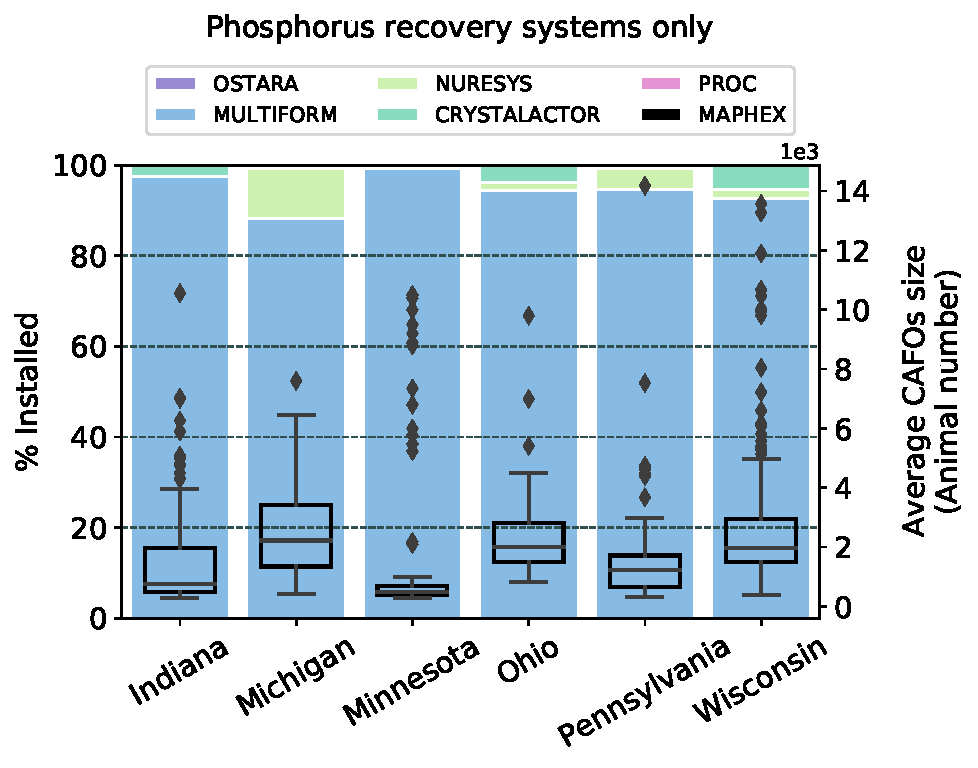
\includegraphics[width=\linewidth]{TechsDistribution_Pcredits22_REC0.pdf} 
		\caption{Phosphorus recovery systems only.}
		\label{fig:PTechs_Distribution_NoAD}
	\end{subfigure}
	\quad
	\begin{subfigure}[t]{0.49\linewidth}
		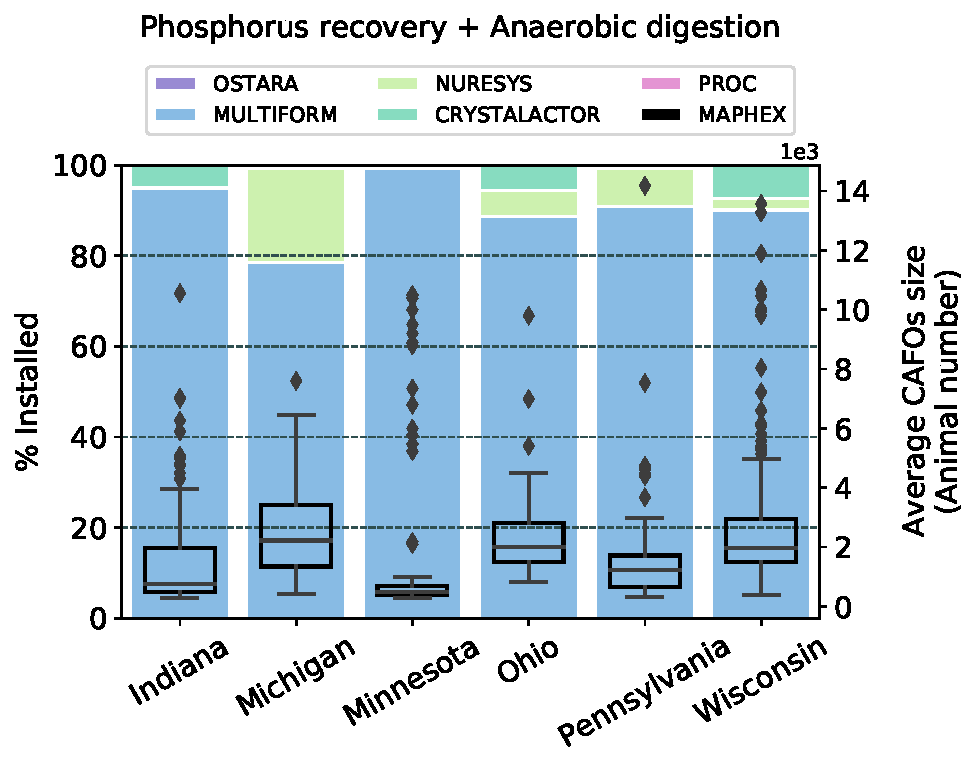
\includegraphics[width=\linewidth]{TechsDistribution_Pcredits22_REC60.pdf}
		\caption{Phosphorus recovery systems coupled with AD and electricity production.}
		\label{fig:PTechs_Distribution_AD}
	\end{subfigure}
	
	\caption{Distribution of the phosphorus recovery systems selected for the CAFOs in the Great Lakes area. The boxplots represent the distribution of CAFO sizes in each studied state.}
	\label{fig:PTechs_Distribution}
\end{figure}

Based on the data illustrated in Figures \ref{fig:Capital_TechSelected} to \ref{fig:NetRev_TechSelected}, a preliminary screening of P recovery systems can be performed based on the size of the CAFOs. If the installation of only nutrient recovery systems is considered, Multiform can be selected for CAFOs with sizes up to 5,000 animal units, NuReSys can be selected for CAFOs with a size between 2,000 and 5,000 animal units, and Crystalactor is selected for CAFOs larger than 5,000 animal units. For the scenario integrating anaerobic digestion and phosphorus recovery processes, Multiform is mostly selected for CAFOs up to 4,000 animal units, although it is also selected in some larger CAFOs, NuReSys are mostly selected for CAFOs between 2,000 and 6,000 animal units, while the size range for the selection of Crystalactor is similar to the previous case. The operating costs are shown in Figure \ref{fig:OPEX_TechSelected}. It can be observed that the operating cost of Multiform is larger than NuReSys, and in turn the operating cost of this one is larger than Crystalactor, showing an opposite pattern than capital costs.

\subsubsection{Effect of local eutrophication risk on the selection of P recovery systems}
The results obtained reveal that CAFOs scale is the main driver for the selection of phosphorus recovery technologies. However, the role of the environmental vulnerability to eutrophication can be appreciated in those CAFOs where two different systems show similar economic performance. From the results illustrated in Figure \ref{fig:NetRev_TechSelected}, it can be observed that Multiform and NuReSys technologies are selected for CAFOs with similar size. However, the economic performance of the second technology is better
%as shown in Figure 
%The net revenue of the manure management systems installed, according with the economic parameters described at the beginning of the section, are shown in Figure
%\ref{fig:NetRev_TechSelected}, 
as consequence of the lower operating expenses and larger net revenues of this technology. Although both technologies have similar phosphorus recovery yield, Multiform shows better environmental performance since the eutrophication potential of its output streams is lower than NuReSys effluents. This difference in eutrophication potential between both technologies is mainly driven by the higher nitrogen recovery of Multiform. Therefore, in those locations that are highly vulnerable to nutrient pollution, the solution proposed by the COW2NUTRIENT framework is driven more by environmental criteria than by economic criteria, resulting in the selection of the Multiform process.


%\begin{table}[h]
%	\centering
%	\caption{Distribution and characteristics studied CAFOs, and phosphorus recovery processes selected. Only selected technologies are included in the table.} \label{table:techs_intalled}
%	\begin{threeparttable}
%		\resizebox{\columnwidth}{!}{
%			\begin{tabular}{@{}cccccccccc@{}}
%				\toprule
%				\multirow{3}{*}{State} & \multirow{3}{*}{\begin{tabular}[c]{@{}c@{}}{\color{blue}CAFO}\\ average size\\ (Animal units)\end{tabular}} & \multirow{3}{*}{\begin{tabular}[c]{@{}c@{}}Number\\ of CAFOs\end{tabular}} & \multirow{3}{*}{\begin{tabular}[c]{@{}c@{}}Total animal \\ units \\ ($10^{-3}$)\end{tabular}} & \multicolumn{6}{c}{\begin{tabular}[c]{@{}c@{}}Number of phosphorus\\ recovery systems installed\end{tabular}} \\ \cmidrule(l){5-10} 
%				&                                                                                                &                                                                            &                                                                                       & \multicolumn{2}{c}{Multiform}       & \multicolumn{2}{c}{NuReSys}       & \multicolumn{2}{c}{Crystalactor}  \\ \cmidrule(lr){5-6} \cmidrule(lr){7-8} \cmidrule(lr){9-10}
%				&                                                                                                &                                                                            &                                                                                       & S1               & S2               & S1              & S2              & S1              & S2              \\ \midrule
%				Indiana           & 1,574.41                                                                                        & 119                                                                         & 187.355                                                                                & 116               & 113               & 0               & 0               & 3               & 6               \\
%				Michigan          & 2,461.52                                                                                        & 144                                                                        & 354.460                                                                                & 127              & 113               & 16              & 30              & 1               & 1               \\
%				Minnesota         & 634.23                                                                                        & 1,487                                                                         & 943.094                                                                                & 1,477                & 1,476                & 0               & 0               & 10              & 11              \\
%				Ohio              & 2,415.24                                                                                        & 53                                                                         & 128.008                                                                                & 50               & 47               & 1               & 3               & 2               & 3               \\
%				Pennsylvania      & 1,495.94                                                                                        & 131                                                                         & 191.967                                                                                & 124               & 119               & 6               & 11              & 1               & 1               \\
%				Wisconsin         & 2,628.19                                                                                        & 283                                                                        & 743.777                                                                                & 262              & 255              & 6               & 7              & 15              & 21              \\ \bottomrule
%		\end{tabular}}
%		\begin{tablenotes}
%			\item S1: Phosphorus recovery systems only.
%			\item S2: Phosphorus recovery systems coupled with AD and electricity production.
%		\end{tablenotes}
%	\end{threeparttable}
%\end{table}

%The relationship between CAFOs size and technologies selected can be better explained through the Figure \ref{fig:PTechs_Distribution}, which illustrates the distribution of technologies selected {\color{blue}{in each studied state.}}
%%for the studied CAFOs. 
%{\color{blue}{The}} size distribution of CAFOs from each studied state is represented through boxplots. It can be observed that in those states with smaller CAFOs, such as Minnesota and Indiana, the selection of Multiform is more predominant than in the states with larger CAFOs. On the contrary, in the states with large CAFOs or with outliers representing big facilities, including Ohio, and Wisconsin, Crystalactor is selected for some facilities. Finally, NuReSysis is a technology also selected in states with medium-size facilities, including Michigan, Ohio, Pennsylvania, and Wisconsin.

%Since the technologies selected are mainly based on the production of struvite, the phosphorus recovery efficiency is around 78 \% of the total phosphorus released in all the studied states.
%The results obtained can be found in the Table 11S of the Supplementary Material.

\subsection{Economic results}
The capital expenditures (CAPEX), operating expenses (OPEX), and net revenues (difference between incomes and operating expenses) associated with the deployment of the nutrient management systems are listed per state in Table \ref{table:economic_results}. For the scenario considering the installation of only phosphorus recovery processes, the CAPEX and OPEX are 2,540.77 MM USD and 185.65 MM USD per year respectively. If the integration of biogas production and upgrading to power with phosphorus management is considered, the CAPEX and OPEX increase up to 5,192.29 MM USD and 267.51 MM USD per year respectively. It can be observed that, due to the high CAPEX of biogas production and upgrading stages, the net revenues decrease from 230.65 MM USD per year for the scenario considering only phosphorus recovery systems to 95.77 MM USD per year if the processes for phosphorus recovery and AD are combined.

%\begin{table}[h]
%	\centering
%	\caption{Economic results for installing phosphorus recovery systems in the studied states of the Great Lakes area.} \label{table:economic_results}
%	\begin{threeparttable}
%		\resizebox{\columnwidth}{!}{
%		\begin{tabular}{@{}ccccccc@{}}
%			\toprule
%			\multirow{2}{*}{State} & \multicolumn{2}{c}{\begin{tabular}[c]{@{}c@{}}Capital expenditure\\ (MM USD)\end{tabular}} & \multicolumn{2}{c}{\begin{tabular}[c]{@{}c@{}}Operating expenditure\\ (MM USD/year)\end{tabular}} & \multicolumn{2}{c}{\begin{tabular}[c]{@{}c@{}}Operating expenditure including \\ equipment amortization\\ (MM USD/year)\end{tabular}} \\ \cmidrule(lr){2-3} \cmidrule(lr){4-5} \cmidrule(lr){6-7} 
%			& S1                                          & S2                                          & S1                                           & S2                                           & S1                                                             & S2                                                             \\ \midrule
%			Indiana                & 145.58                                       & 325.00                                      & 14.25                                        & 18.64                                        & 21.18                                                          & 34.16                                                          \\
%			Michigan               & 191.09                                      & 480.19                                      & 27.64                                        & 33.05                                        & 36.74                                                          & 55.92                                                          \\
%			Minnesota              & 1,591.40                                       & 2,866.31                                      & 64.96                                         & 115.09                                        & 140.74                                                           & 251.58                                                          \\
%			Ohio                   & 68.30                                       & 179.29                                      & 9.70                                         & 11.78                                        & 12.95                                                          & 20.32                                                          \\
%			Pennsylvania           & 148.16                                       & 332.03                                      & 14.41                                        & 19.22                                        & 21.46                                                          & 35.03                                                          \\
%			Wisconsin              & 396.24                                      & 1,009.47                                      & 54.69                                        & 69.73                                        & 73.55                                                          & 117.80                                                         \\ \bottomrule
%		\end{tabular}}
%		\begin{tablenotes}
%			\item S1: Phosphorus recovery systems only.
%			\item S2: Phosphorus recovery systems coupled with AD and electricity production.
%		\end{tablenotes}
%	\end{threeparttable}
%\end{table}

\begin{table}[h]
	\centering
	\caption{Economic results per state for installing phosphorus recovery systems in the studied states of the Great Lakes area.} \label{table:economic_results}
	\begin{threeparttable}
%		\resizebox{\columnwidth}{!}{
			\begin{tabular}{@{}ccccccc@{}}
				\toprule
				\multirow{2}{*}{State} & \multicolumn{2}{c}{\begin{tabular}[c]{@{}c@{}}CAPEX\\ (MM USD)\end{tabular}} & \multicolumn{2}{c}{\begin{tabular}[c]{@{}c@{}}OPEX\\ (MM USD/year)\end{tabular}} & \multicolumn{2}{c}{\begin{tabular}[c]{@{}c@{}}Net revenue\\ (MM USD/year)\end{tabular}} \\ \cmidrule(lr){2-3} \cmidrule(lr){4-5} \cmidrule(lr){6-7} 
				& S1                                          & S2                                          & S1                                           & S2                                           & S1                                                             & S2                                                             \\ \midrule
				Indiana                & 145.58                                       & 325.00                                      & 21.18                                        & 34.16                                        & 19.32                                                          & 11.88                                                          \\
				Michigan               & 191.09                                      & 480.19                                      & 36.74                                       & 55.92                                        & 41.00                                                          & 32.15                                                          \\
				Minnesota              & 1,591.40                                       & 2,866.31                                      & 140.74                                         & 251.58                                        & 39.61                                                           & -46.15                                                          \\
				Ohio                   & 68.30                                       & 179.29                                      & 12.95                                         & 20.32                                        & 14.46                                                          & 10.80                                                          \\
				Pennsylvania           & 148.16                                       & 332.03                                      & 21.46                                        & 35.03                                       & 20.82                                                          & 12.95                                                          \\
				Wisconsin              & 396.24                                      & 1,009.47                                      & 73.55                                        & 117.80                                        & 95.44                                                          & 74.14                                                         \\ \bottomrule
		\end{tabular}
%	}
		\begin{tablenotes}
			\item S1: Phosphorus recovery systems only.
			\item S2: Phosphorus recovery systems coupled with AD and electricity production.
		\end{tablenotes}
	\end{threeparttable}
\end{table}



% associated with the  between the different phosporus recovery systems. This is a consequence the larger scale of the manure treatment processes integrating anaerobic digestion, biogas valorization, and nutrient recovery stages, resulting in considerable larger investment and operating costs. Therefore, as shown in Figure ?? a result, the integration of  the costs differences among nutrient recovery technologies are blurred into the costs of the whole process.

% Multiform is the predominant technology for CAFOs with a size up to 3000 animal units, while Crystalactor is the technology selected for CAFOs bigger than 7500. For CAFOs between 3000 and 7500 animal units NuReSys is the system with the best performance. Figure ?? shows the average CAFOs size and the average distribution of phosphorus recovery technologies installed in the states studied. It can be observed that the states with small CAFOs have a larger fraction of Multiform facilities, while the installation of NuReSys and Crystalactor processes is more often in the states with larger CAFOs. 
 
% In addition, it can be observed that the integration of anaerobic digestion and electricity generation stages affects the economies of scale, reducing the differences of capital and operating costs between the different nutrient recovery systems. This is due to the larger scale of the manure treatment processes integrating anaerobic digestion, biogas valorization, and nutrient recovery stages, resulting in considerable larger investment and operating costs. As a result, the costs differences among nutrient recovery technologies are blurred into the costs of the entire process. Therefore, the transition range between technologies is larger when the integration of anaerobic digestion and biogas valorization stages are considered, Figure \ref{fig:PTechs_Distribution_AD}, than if only the installation of nutrient recovery processes is considered, Figure \ref{fig:PTechs_Distribution_NoAD}. 

\begin{figure}[H]
	\begin{subfigure}[t]{0.48\linewidth}
		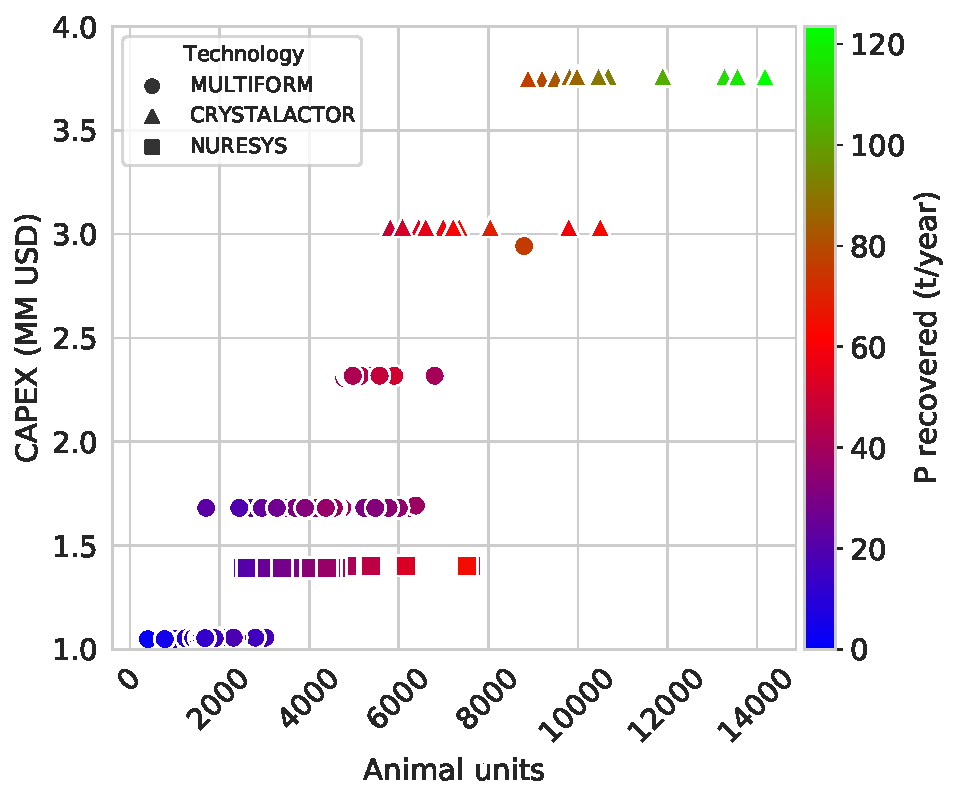
\includegraphics[width=\linewidth]{Capital_TechSelected_Pcredits22_REC0.pdf} 
		\caption{Phosphorus recovery systems only.}
		\label{fig:Capital_TechSelected_Pcredits22_REC0}
	\end{subfigure}
	\quad
	\begin{subfigure}[t]{0.48\linewidth}
		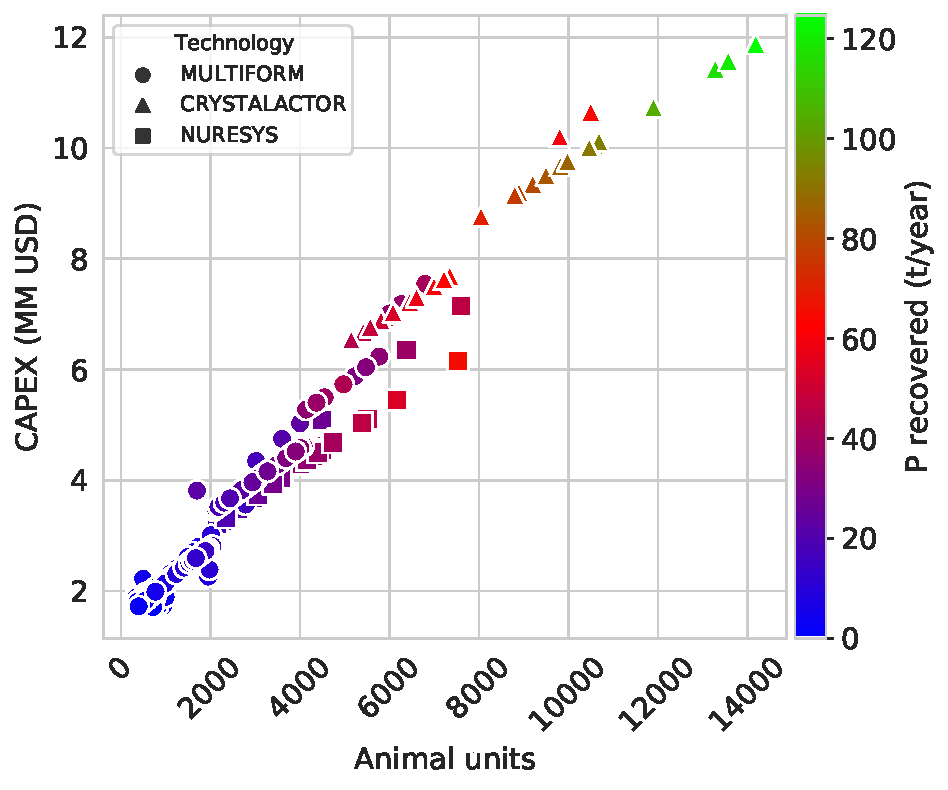
\includegraphics[width=\linewidth]{Capital_TechSelected_Pcredits22_REC60.pdf}
		\caption{Phosphorus recovery systems coupled with AD and electricity production.}
		\label{fig:Capital_TechSelected_Pcredits22_REC60}
	\end{subfigure}
	
	\caption{Capital expenses for deploying phosphorus recovery systems in the studied CAFOs. The dots represent the P recovery technologies installed in the studied CAFOs.}
	\label{fig:Capital_TechSelected}
\end{figure}


\begin{figure}[H]
	\begin{subfigure}[t]{0.48\linewidth}
		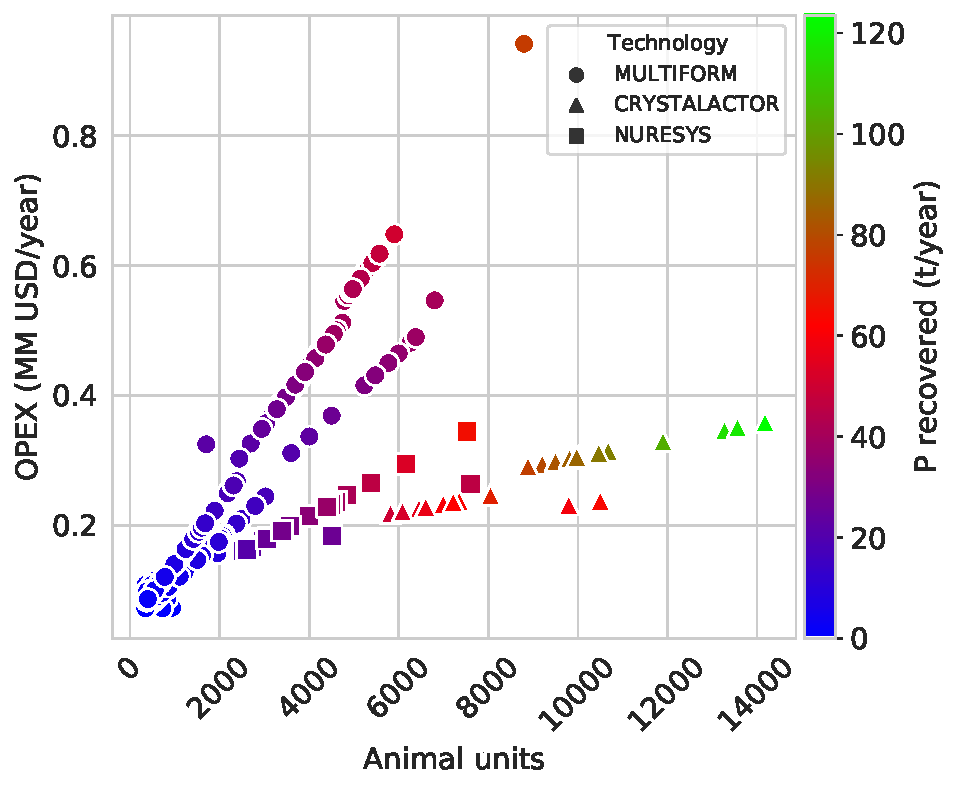
\includegraphics[width=\linewidth]{Amortized_TechSelected_Pcredits22_REC0.pdf} 
		\caption{Phosphorus recovery systems only.}
		\label{fig:OPEX_TechSelected_Pcredits22_REC0}
	\end{subfigure}
	\quad
	\begin{subfigure}[t]{0.48\linewidth}
		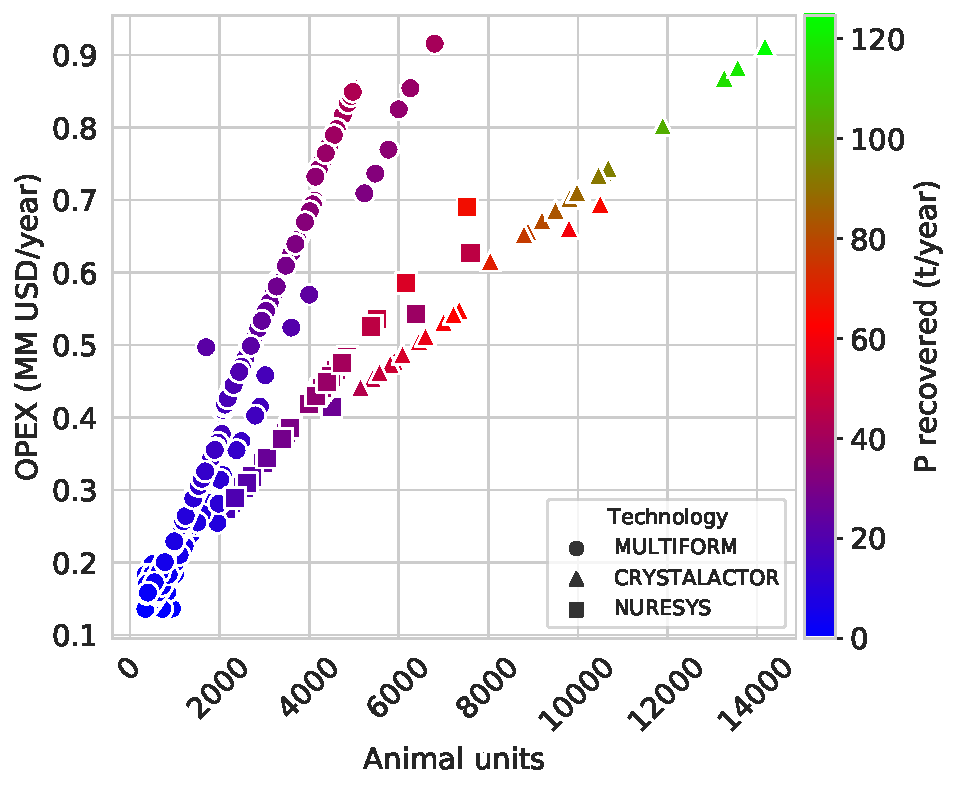
\includegraphics[width=\linewidth]{Amortized_TechSelected_Pcredits22_REC60.pdf}
		\caption{Phosphorus recovery systems coupled with AD and electricity production.}
		\label{fig:OPEX_TechSelected_Pcredits22_REC60}
	\end{subfigure}
	
	\caption{Operating expenses for deploying phosphorus recovery processes in the studied CAFOs. The dots represent the P recovery technologies installed in the studied CAFOs.}
	\label{fig:OPEX_TechSelected}
\end{figure}

Figures \ref{fig:Capital_TechSelected} and \ref{fig:OPEX_TechSelected} show the evolution of CAPEX and OPEX of the P recovery technologies installed at the livestock facilities studied as a function of CAFOs scale. Figure \ref{fig:Capital_TechSelected_Pcredits22_REC0} shows the CAPEX when the implementation of only P recovery systems is considered. We observe that CAFOs are grouped in sets selecting the same P recovery technology. This is because the manufacturers standardize the size of each P recovery technology, which in turn determines the maximum waste processing capacity of each technology (as shown in Table \ref{table:techs_description}). This results in the use of the same P recovery equipment, and thus the same CAPEX, for all the CAFOs generating waste below the maximum processing capacity.
% Therefore, each technology can process an amount waste equal or below its maximum capacity, resulting  range. Since the sizes are normalized, this results in the same CAPEX for the range of CAFOs size generating an amount of waste equal or below the maximum processing capacity of the technology, as the reviewer points out.		
Likewise, we note different CAPEX values for the implementation of the same P recovery technology. This is a consequence of installing of multiple in-parallel P recovery units to increase the processing capacity of such technology, since the waste generated in that CAFO exceeds its maximum processing capacity.
%It is worth noting that the installation of multiple P recovery units to increase the processing capacity of the process can be observed in Figure \ref{fig:Capital_TechSelected_Pcredits22_REC0}, where {\color{blue}{Multiform}} technology can be appreciated at different CAPEX {\color{blue}{values}}. This is consequence of the installation of multiple parallel units to increase the capacity of the facility. 
%It can also be observed that different numbers of P recovery units of the same technology are installed for similar size CAFOs. 
It can also be appreciated that CAFOs with similar size might result in the installation of different technologies, or a different number of units of the same technology.
This is because, although CAFOs can have a similar number of animal units, the type of the animals can be different, resulting in the generation of different amounts of manure. 
In the case of considering biogas production and upgrading, illustrated in Figure \ref{fig:Capital_TechSelected_Pcredits22_REC60}, the required CAPEX increases significantly, blurring the differences in the capital investment between different P recovery processes observed in Figure \ref{fig:Capital_TechSelected_Pcredits22_REC0} into the cost of the whole system. The integration of AD and electricity production also results in the increase of the OPEX, as shown in Figure \ref{fig:OPEX_TechSelected}.

\begin{figure}[H]
	\begin{subfigure}[t]{0.48\linewidth}
		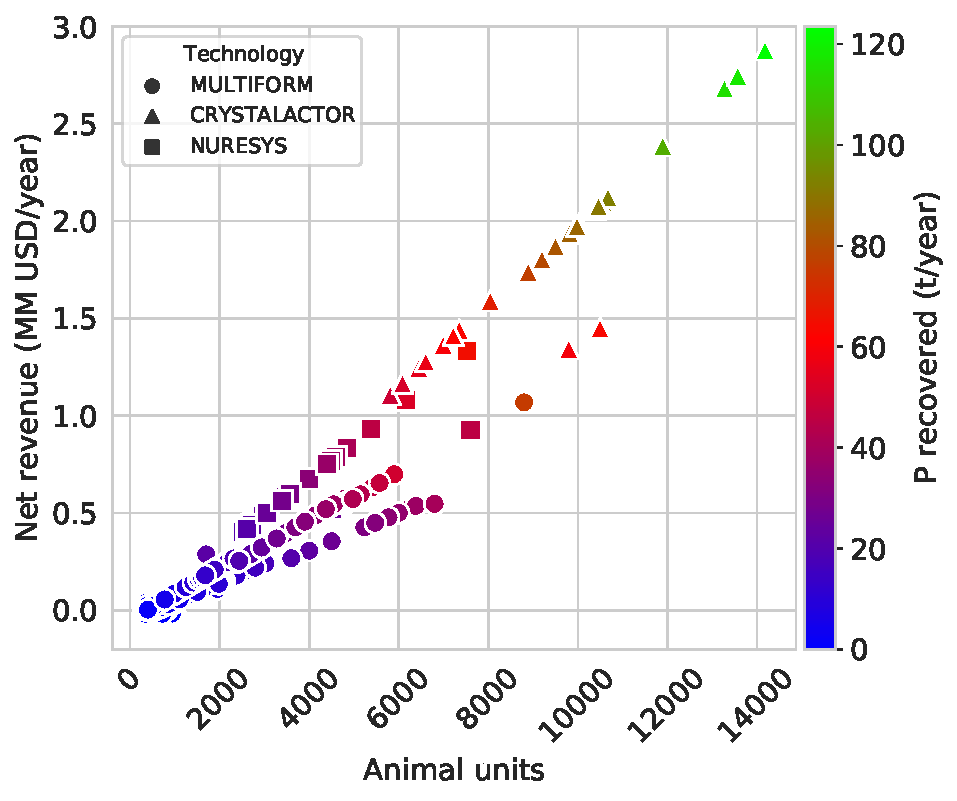
\includegraphics[width=\linewidth]{NetRev_TechSelected_Pcredits22_REC0.pdf} 
		\caption{Phosphorus recovery systems only.}
		\label{fig:NetRev_TechSelected_Pcredits22_REC0}
	\end{subfigure}
	\quad
	\begin{subfigure}[t]{0.48\linewidth}
		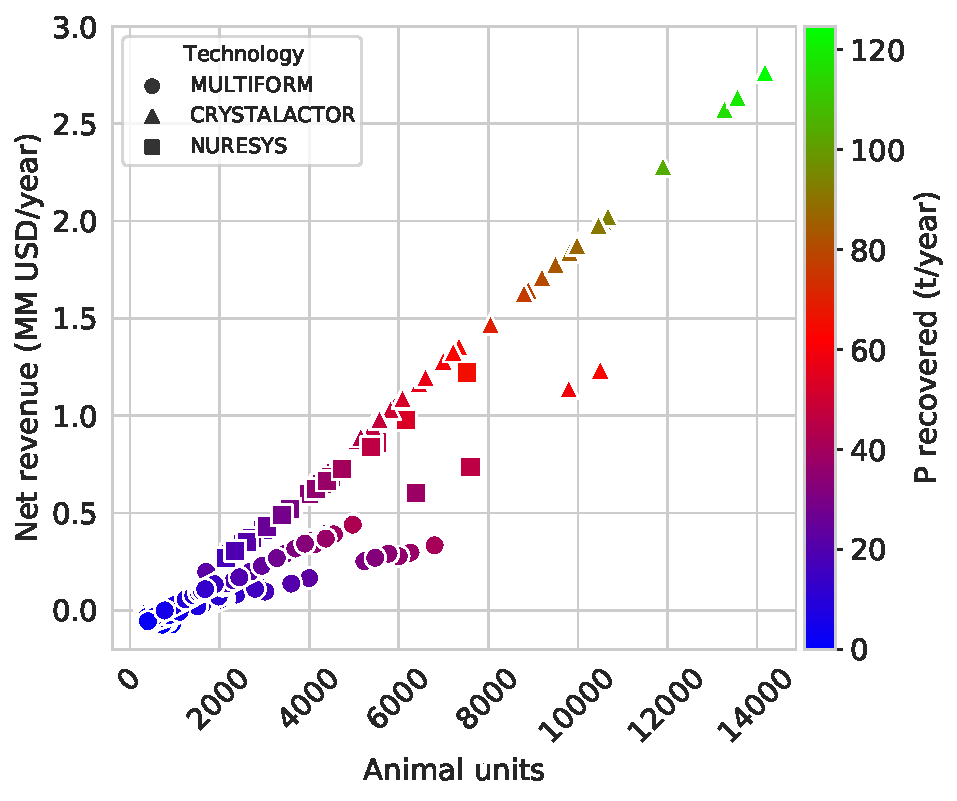
\includegraphics[width=\linewidth]{NetRev_TechSelected_Pcredits22_REC60.pdf}
		\caption{Phosphorus recovery systems coupled with anaerobic digestion and electricity production.}
		\label{fig:NetRev_TechSelected_Pcredits22_REC60}
	\end{subfigure}
	
	\caption{Net revenue from the phosphorus recovery processes selected in the studied CAFOs. The dots represent the P recovery technologies installed in the studied CAFOs.}
	\label{fig:NetRev_TechSelected}
\end{figure}

The net revenue of the installed nutrient management systems according with the economic parameters described at the beginning of the section is shown in Figure \ref{fig:NetRev_TechSelected}. We observe a pattern characterized by the increase of the net revenues with the increase of CAFOs size. However, the implementation of P recovery technologies in CAFOs below 1,000 animal units, and below 2,000 animal units if biogas production and upgrading is also considered, result in economic looses. Additionally, the integration of these processes slightly decreases the net revenues of the systems installed for phosphorus recovery.


%From the obtained results, it can be observed that Multiform and NuReSys are systems selected for facilities with similar size. The economic performance of the second technology is better
%%as shown in Figure 
%%The net revenue of the manure management systems installed, according with the economic parameters described at the beginning of the section, are shown in Figure
%%\ref{fig:NetRev_TechSelected}, 
%as consequence of the lower operating expenses and lower capital cost of this technology. Although both technologies have a similar phosphorus recovery yield, it must be noted that Multiform shows a better environmental performance since the eutrophication potential of the process output streams is lower than the eutrophication potential of NuReSys. Therefore, for those locations that are highly vulnerable to nutrient pollution, the solution proposed by the COW2NUTRIENT framework is more driven by environmental criteria than by economic criteria. As a consequence of the economies of scale of CAFOs, the selection of modular phosphorus recovery systems such as MAPHEX, which are specially indicated for small livestock facilities, is largely prevented by the absence of small livestock facilities.

%It should be noted that the selection of nutrient management processes including modular nutrient recovery systems such as MAPHEX, which are specially indicated for small livestock facilities, is largely prevented by the absence of small CAFOs.
% but a trade-off between environmental criteria and long-term plan operation feasibility is pursued.r sizes.
% NuReSys shows a better economic performance, while Multiform shows a better environmental performance. Therefore, for these the technology selection will be driven by the environmental vulnerability to nutrient pollution of the watershed where the CAFO studied is located, determining whether environmental or economic criteria is prioritized.



\section{Discussion}
%{\color{blue}{\subsection{Implications at CAFO level}}}
%{\color{blue}{\subsubsection{Relevance of MCDA criteria in the selection of P recovery systems}}}
%Currently, manure or digestate in liquid phase is usually supplied as nutrient supplementation in croplands, or it is treated in either aerobic or anaerobic ponds. Solid phase processing is based on composting or drying. However, the high density of manure and digestate and the relatively low amount of nutrients compared to their total mass of organic waste prevent an efficient redistribution of the phosphorus released at CAFOs to phosphorus-deficient areas. Therefore, the implementation of phosphorus recovery processes 
%%is a desirable measure for sustainable phosphorus management, 
%mitigate nutrient pollution of waterbodies at the time that phosphorus is efficiently redistributed to nutrient depleted locations. 
%However, the P recovery technologies available result in the recovery of different products and operating costs. Therefore, the selection of the most suitable processes for CAFOs is addressed evaluating a set of five criteria.

%The criteria considered fall into three categories: environmental vulnerability to eutrophication, economic performance, and technological readiness level (TRL). The TRL is the first criteria considered in order to minimize the risk of selecting non-full-scale processes.
%% unless they show to be very advantageous in the economic or environmental dimensions. 
%%As a consequence, TRL result in a preliminary screening of the technologies.
%Therefore, the selection of processes with low TRL will be hampered unless they have good economic or environmental performances.  
%
%Regarding environmental and economic criteria, these are prioritized based on the eutrophication risk of the subbasin studied. However, the results reveal that only three of the technologies studied are selected through all the CAFOs assessed (i.e., Multiform, Nuresys, and Crystalactor). These technologies recover phosphorus through struvite production, which is a valued product that can be sold, generating income. Although the Ostara Pearl process also produces struvite, it results in larger operating costs than the technologies selected. Conversely, P-RoC recovers phosphorus in the form of calcium-based precipitates. This product lacks a well-established market, and therefore it does not generate income. In addition, P-RoC is the technology with the lowest TRL, which hampers the selection of this process. The selection of modular phosphorus recovery systems, such as MAPHEX, which due to economies of scale are especially suitable for small livestock facilities, is largely prevented by the absence of small-scale CAFOs. Therefore, a sub-set of three technologies is obtained. Therefore, it can be concluded that the selection of this pool of three technologies amongst the six systems evaluated is mainly driven by economic factors. Additionally, the low TRL of P-RoC also hampers the selection of this process.
%
%The selection of the most suitable technology for each studied CAFO among the sub-set comprised by Multiform, Nuresys, and Crystalactor systems is based on the CAFO scale and local eutrophication risk, as it is discussed in the next sections.
%
%{\color{blue}{\subsubsection{Effect of CAFOs scale on the selection of P recovery systems}}}
%%By comparing Figures \ref{fig:PTechs_Distribution_NoAD} and \ref{fig:PTechs_Distribution_AD}
%%%, which illustrate the selection of technologies for both of scenarios assessed, 
%%it can be observed that the integration of AD and electricity generation stages promotes the selection of {\color{blue} {processes that require larger investment costs, such as}} NuReSys and Crystalactor technologies. 
%%{\color{blue}{This is because the capital costs of biogas production and upgrading processes are significantly larger than the capital costs of P recovery technologies, as it can be observed in Table \ref{table:economic_results}. Therefore, the differences of capital expenses among different phosphorus recovery technologies are blurred into the costs of the whole system (i.e., biogas production and upgrading, and P recovery processes).}}
%%%Therefore, {\color{blue} {the effect of the economies of scale is increased by the integration of AD processes with phosphorus recovery processes}} as a result of.
%%%Since the integration of these stages involves large capital costs, the differences of capital expenses among different phosphorus recovery technologies are blurred into the costs of the whole process, as shown in Figure \ref{fig:Capital_TechSelected}.  
%%As a result, a larger number of NuReSys and Crystalactor processes are selected because of their lower operating costs, as shown in Figure \ref{fig:OPEX_TechSelected}. Additionally, the relationship between the processes selected and size of CAFOs (number of animal units) described previously can be observed in Figure \ref{fig:Capital_TechSelected}. 
%
%Based on the data illustrated {\color{blue}{in Figures \ref{fig:Capital_TechSelected} to \ref{fig:NetRev_TechSelected},}} CAFO size ranges for the selection or discard of phosphorus recovery technologies can be proposed. If the installation of only nutrient recovery systems is considered, Multiform can be selected for CAFOs with sizes up to 5,000 animal units, NuReSys can be selected for CAFOs with a size between 2,000 and 5,000 animal units, and Crystalactor is selected for CAFOs larger than 5,000 animal units. For the scenario integrating anaerobic digestion and phosphorus recovery processes, Multiform is mostly selected for CAFOs up to 4,000 animal units, although it is also selected in some larger CAFOs, NuReSys are mostly selected for CAFOs between 2,000 and 6,000 animal units, while the size range for the selection of Crystalactor is similar to the previous case. The operating costs are shown in Figure \ref{fig:OPEX_TechSelected}. It can be observed that, due to the technology used in each process, the operating cost of Multiform is larger than NuReSys, and in turn the operating cost of this one is larger than Crystalactor, showing an opposite pattern than capital costs.
%
%{\color{blue}{\subsubsection{Effect of local eutrophication risk on the selection of P recovery systems}}}
%The results obtained reveal that CAFOs scale is the main driver for the selection of phosphorus recovery technologies. However, the role of the environmental vulnerability to eutrophication can be appreciated in those {\color{blue}{CAFOs}} where two different systems show similar economic performance. From the results illustrated in Figure \ref{fig:NetRev_TechSelected}, it can be observed that Multiform and NuReSys technologies are selected for CAFOs with similar size. However, the economic performance of the second technology is better
%%as shown in Figure 
%%The net revenue of the manure management systems installed, according with the economic parameters described at the beginning of the section, are shown in Figure
%%\ref{fig:NetRev_TechSelected}, 
%as consequence of the lower operating expenses and lower capital cost of this technology. Although both technologies have similar phosphorus recovery yield, Multiform shows better environmental performance since the eutrophication potential of its output streams is lower than NuReSys effluents. Therefore, in those locations that are highly vulnerable to nutrient pollution, the solution proposed by the COW2NUTRIENT framework is driven more by environmental criteria than by economic criteria, resulting in the selection of the Multiform process. 
%
%{\color{blue}{\subsection{Implications at state level}}}
\subsection{Economic implications}
In this work, fixed incentives for P recovery and biogas-based electricity generation have been considered as starting point to explore the effect of the application of incentives in the implementation of P recovery technologies, either standalone or integrated with biogas production and upgrading processes.		
The results shown in Figure \ref{fig:NetRev_TechSelected} reveal the effect of the economies of scale in the net revenues from the implementation of P recovery technologies in the Great Lakes area are highly dependent on the economies of scale, i.e., the larger the amount of waste to be treated, the larger the net revenues obtained. However, while for the largest CAFOs significant profits are obtained, negative revenues (i.e., economic looses) are obtained for the smallest CAFOs, even for large P credits prices such as 22 USD/kg\textsubscript{P recovered}. This suggests that the implementation of fixed incentives is not a fair policy, since the small CAFOs are not profitable while they increase the profits of the largest CAFOs. Therefore, alternative incentive policies must be explored. \citet{sampat2019coordinated} studied the development of a coordinated management system for the treatment of cattle manure and P recovery. That framework captures the geographical phosphorus imbalance by proposing different prices for manure treatment that capture the regional remediation cost caused by P releases. They found that economic drivers are needed for a cost-effective recovery and redistribution of phosphorus, considering fixed incentives for P recovery up to 50 USD/kg\textsubscript{P} for this purpose. Therefore, further research about the effect of implementing dynamic incentives for P recovery is needed. These incentive policies can follow different schemes, such as progressive incentives for P recovery based on the amount of manure treated, or cooperative schemes where the profits from P recovery obtained by the largest livestock facilities are redistributed to the smallest CAFOs. This is a concept that has been studied for minimizing the costs of meeting greenhouse gases emission targets \citep{galan2018time}, and could be adopted for the reduction of P releases.

Furthermore, consideration should be given to the fair allocation of incentives in those scenarios where the available incentives budget is not enough to avoid economic looses in all CAFOs. In this regard, the fairness measure considered for budget allocation must be carefully selected among the existing schemes \citep{sampat2019fairness}. 
%As a result, we note that the following three factors should be considered in the design of incentive schemes: avoiding economic looses in all CAFOs, a fair distribution of the available incentives, and minimizing the cost of the incentives required in order to reduce the social impact of P recovery while mitigating environmental impacts.}}

\subsection{Phosphorus use efficiency}
Currently, manure or digestate in liquid phase is usually supplied as nutrient supplementation in croplands, or it is treated in either aerobic or anaerobic ponds. Solid phase processing is based on composting or drying. However, the high density of manure and digestate and low concentration of nutrient prevent an efficient redistribution of the phosphorus released from CAFOs to phosphorus-deficient areas \citep{burns2002phosphorus}. Therefore, the implementation of phosphorus recovery processes 
is a desirable measure for sustainable phosphorus management. 
%mitigate nutrient pollution of waterbodies at the time that phosphorus is efficiently redistributed to nutrient depleted locations. 
We find that implementing struvite production processes considering incentives for P recovery of 22 USD/kg\textsubscript{P recovered} is economically feasible for CAFOs larger than 1,000 animal units if standalone P recovery technologies are implemented, and for CAFOs larger than 2,000 animal units if they are integrated with biogas production and upgrading processes. The requirement of large incentives to produce profit in most of the P recovery systems installed at CAFOs might raise the debate of whether it is worthwhile to implement P recovery systems; or if the economic resources should be allocated to simpler phosphorus management alternatives, such as the redistribution of either raw or pond-stored manure. In this regard, \citet{sampat2019coordinated} studied the separation of manure in liquid and solid phases, and their further transport to demanding allocations, considering a coordinated management system in Upper Yahara watershed (Wisconsin, United States). In addition, that study considered the implementation of economic incentives from 0 to 50 USD/kg\textsubscript{P}. However, the results showed that manure redistribution is not an economically viable technique for phosphorus recycling in this range of incentives. The main drawback of manure redistribution is the large transportation cost of both liquid and solid raw manure because of the high volume of these materials and their low phosphorus concentration. Therefore, the results reveal that on-site manure processing to generate valuable products (struvite) is more beneficial than manure redistribution.

%Phosphorus recovery from livestock manure allows for phosphorus recycling and redistribution. Therefore,
The replacement of phosphorus from synthetic fertilizers by the recovered P, mitigating the dependency on fertilizers from non-renewable resources (phosphate rock), is an interesting alternative towards the sustainability of the agri-food sector. However, phosphorus availability for plants depends on several factors, including the P product used as fertilizer and soil pH level. Since struvite is the product recovered in all studied CAFOs, we will focus the discussion on this product.
%Therefore, to quantify the amount of synthetic fertilizers that could be replaced by P recovered from livestock manure is not a straight forward procedure. 
\citet{vaneeckhaute2015efficiency} compared the bio-availability of several bio-based fertilizers, including struvite, to synthetic triple super phosphate (TSP). This study shows that P available in soil (measured as Prhizon) was a 45\% higher than TSP in acidic soils (pH=5.0), but 60\% lower in slightly basic soils (pH=7.9). Based on these data, one kilogram of manure processed for P recovery by struvite production can replace from $1.53\cdot 10^{-3}$ to $3.71\cdot 10^{-3}$ kg of TSP ($5.02 \cdot 10^{-3}$ kg of struvite are recovered per kilogram of manure processed). However, it must be noted that currently the cost of recovered P from manure (2.12-15.42 USD/kg\textsubscript{P recovered}, see Table \ref{table:techs_description}) is considerable larger than the cost of phosphorus from synthetic TSP (1.23  USD/kg\textsubscript{P}) \citep{fertilizers_price}. As a result, from an economic perspective the complete substitution of phosphate rock is currently hindered by the large recovery costs, in addition to a limited availability of resources recovered from waste, and henceforth further exploration on resource recovery from different wastes is required to achieve P circularity reducing the recovery costs, and increasing the amount of phosphorus from organic waste, including but not limited to livestock manure.

%{\color{red}{??}}  kg of phosphorus are recovered per kilogram of manure processed. This avoids the use of {\color{red}{??}} kilograms of {\color{red}{superphosphate}}, a common material used for P supplementation on croplands. However, it must be noted that currently the cost of recovered P from manure ({\color{red}{??}}) is considerable larger than {\color{red}{ syntheticsuperphosphate}} ({\color{red}{??}}). Therefore, the complete substition of phosphate rock is currently hindered by the large recovery costs, and henceforth further exploration on resource recovery from different wastes is required to achieve P circularity.

%
%\subsection{Effect of CAFOs scale on P recovery cost}
%
%\subsection{Effect of eutrophication risk in on P recovery cost}
%
%
% 
%%Additionally, the reliability of the results obtained depends on the uncertainty in the input data, which increases at smaller scales. A HUC8 spatial resolution has been chosen as a trade-off solution between spatial accuracy and data uncertainty. However, more accurate results can be obtained if reliable data for phosphorus level in soils, fertilizer rates, etc. are available for higher spatial resolution.
%
%%The installation of nutrient recovery systems with and without the integration of anaerobic digestion and electricity generation stages has been studied. 
%
%
%
%
%\subsection{Evaluation of a typical dairy concentrated animal feeding operation}
%The use of the COW2NUTRIENT tool is illustrated through the evaluation of a large size dairy CAFO, defined by US EPA as animal concentrated operations with more than 1,000 animals \citep{CAFO_definition}. To define a representative large dairy CAFO, data from an average dairy producer U.S. state such as Pennsylvania is considered, determining the base case size to compare the facility as the average animal number of the large dairy CAFOs in Pennsylvania, i.e., 2,145 animal units. To evaluate the influence of environmental indicators (i.e., Trophic State Index, TES indicator, and soil fertility level) two locations in the state of Pennsylvania, with low and high vulnerability to nutrients pollution, were selected, as shown in Table \ref{table:scenarios_individual}. The parameters considered for this case study are the addition of a biogas generation stage with electricity production, a value of Renewable Energy Certificates (electricity selling price) of 60 USD per MWh generated, a phosphorus credits value of 22 USD per kilogram of phosphorus recovered, and a discount rate of 7\% to calculate the NPV. These values are based on optimal values for the operation of hybrid biogas-nutrient recovery plants reported by \citet{sampat_economic_2018}.
%
%\begin{table}[H]
%	\centering
%	\caption{Geographic locations considered in the dairy CAFO assessment. Values for sentivity to nutrient pollution indicators are expressed between parenthesis} \label{table:scenarios_individual}
%	\begin{tabular}{@{}cccccc@{}}
%		\toprule
%		& Longitude & Latitude & \begin{tabular}[c]{@{}c@{}}Trophic State\\ Index\end{tabular}                          & \begin{tabular}[c]{@{}c@{}}TES\\ indicator\end{tabular}                               & \begin{tabular}[c]{@{}c@{}}Soil fertility\\ (M3P ppm)\end{tabular}              \\ \midrule
%		\begin{tabular}[c]{@{}c@{}}Scenario 1\\ (low vulnerability)\end{tabular} & -78.4310  & 39.7910  & \cellcolor[HTML]{a0e147}\begin{tabular}[c]{@{}c@{}}Oligotrophic\\ (35.6)\end{tabular}    & \cellcolor[HTML]{fd6864}\begin{tabular}[c]{@{}c@{}}Saturated\\ (1.22)\end{tabular}      & \cellcolor[HTML]{a0e147}\begin{tabular}[c]{@{}c@{}}Medium\\ (29.1)\end{tabular}   \\
%		\begin{tabular}[c]{@{}c@{}}Scenario 2\\ (high vulnerability)\end{tabular} & -76.2269  & 39.7506  & \cellcolor[HTML]{fd6864}\begin{tabular}[c]{@{}c@{}}Hypereutrophic\\ (70.30)\end{tabular} & \cellcolor[HTML]{a0e147}\begin{tabular}[c]{@{}c@{}}Not saturated\\ (-0.57)\end{tabular} & \cellcolor[HTML]{fd6864}\begin{tabular}[c]{@{}c@{}}Excessive\\ (157)\end{tabular} \\
%		\bottomrule
%	\end{tabular}
%\end{table}
%
%The comparison of the economic results of the cattle waste treatment process for the different nutrient recovery systems evaluated are shown in Table \ref{table:economic_individual}. The capital cost ranges between 3.3 and 5.3 million USD for all nutrient recovery processes, while the differences in the operating costs are much more significant. It can be appreciated how the operating costs considering the capital cost amortization for the most technologically mature processes are lower than the processes with a lower technology readiness level. This fact can be attributed to the process optimization carried out prior to their commercial release. This will be the driving factor making the commercial process profitable contrary to the processes still in stages prior to commercial launch. However, when money depreciation is included in the economic evaluation, using NPV as metric, it can be concluded that all of the evaluated nutrient recovery systems fall below the defined rate of return (7\%), although the commercial technologies achieve better NPV values than P-RoC and MAPHEX processes.
%
%\begin{table}[H]
%	\centering
%	\caption{Analysis of the economic performance for diferent nutrient recovery process topologies} \label{table:economic_individual}
%	\begin{tabular}{@{}cccccc@{}}
%		\toprule
%		& \begin{tabular}[c]{@{}c@{}}Capital cost\\ (M USD)\end{tabular} & \begin{tabular}[c]{@{}c@{}}Operation cost\\ (w/o amortization)\\ (M USD/year)\end{tabular} & \begin{tabular}[c]{@{}c@{}}Operation cost\\ (w/ amortization)\\ (M USD/year)\end{tabular} & \begin{tabular}[c]{@{}c@{}}Net revenue\\ (M USD/year)\end{tabular} & \begin{tabular}[c]{@{}c@{}}NPV\\ (USD)\end{tabular} \\ \midrule
%		Ostara       & 5.33                                                   & 0.185                                                                                & 0.413                                                                               & 0.313                                                        & -0.209                                           \\
%		Multiform    & 3.94                                                   & 0.340                                                                               & 0.502                                                                               & 0.224                                                      & -0.156                                           \\
%		NuReSys      & 3.65                                                   & 0.159                                                                                & 0.307                                                                               & 0.403                                                        & -0.116                                           \\
%		Crystalactor & 5.28                                                   & 0.0776                                                                                 & 0.304                                                                               & 0.423                                                        & -0.191                                           \\
%		P-RoC         & 4.31                                                   & 2.32                                                                               & 2.49                                                                              & -1.96                                                      & -0.485                                           \\
%		MAPHEX       & 3.43                                                   & 2.33                                                                               & 2.47                                                                              & -1.78                                                      & -0.443                                           \\ \bottomrule
%	\end{tabular}
%\end{table}
%
%When the results are analyzed using the proposed MCDA module, Figs. \ref{fig:ranking} and \ref{fig:scores}, it can be observed how the geographic location of the facility influences the selection of technologies. Figure \ref{fig:ranking} shows the ranking of nutrient recovery technologies. The robustness of the results can be observed through the frequency of selecting one technology in a determine ranking position along the SMAA iterations, shown in the figure through the color scale  (0\%-100\%). For the location with low sensitivity to phosphorus pollution, Figure \ref{fig:ranking_scenario1}, where the economic criteria prevails over environmental criteria, a robust solution where NuReSys and Multiform are the two first technologies in the ranking is achieved, showing the best overall performance. However, when the location with high environmental risk is analyzed, Figure \ref{fig:ranking_scenario2}, pursuing a trade-off between environmental criteria and long-term plan operation feasibility, the achieved solution is less robust. Multiform and NuReSys are the technologies on the top of the ranking, but among them there is not a process that clearly prevails over the others since they have the first or the second raking position depending on the normalization-aggregation functions and weight values considered. These results can be analyzed in more detail when the breakdown of the average scores obtained for each technology using the different normalization-aggregation combinations are evaluated, as shown in Figure \ref{fig:scores}. While in scenario 1 it can be observed that the technologies with the highest scores are NuReSys and Multiform, prevailing over the rest of technologies, for scenario 2, four out of six technologies reach a score around 0.9 for most of the normalization-aggregation combinations. Furthermore, the effect of the different levels of compensation between indicators can be observed, where the full compensation level represented by the additive aggregation function retrieve the most homogeneous indexes, while the indexes retrieved by the harmonic function, representing the lower partial compensation level, are more heterogeneous. In both scenarios P-RoC always obtains the lowest score. Therefore, in spite of the raking obtained, as a result of the equity in the scores obtained, the decision about what technology implement for scenario 2 is debatable among the first three technologies retrieved by the ranking.
%
%\begin{figure}[H]
%	\centering
%	\begin{subfigure}[t]{0.49\textwidth}
%		\includegraphics[width=\textwidth]{scenario1_ranking}
%		\caption{Scenario 1}
%		\label{fig:ranking_scenario1}
%	\end{subfigure}
%	%	\quadFigure \ref{fig:ranking}
%	\begin{subfigure}[t]{0.49\textwidth}
%		\includegraphics[width=\textwidth]{scenario2_ranking} 
%		\caption{Scenario 2}
%		\label{fig:ranking_scenario2}
%	\end{subfigure}
%	
%	\caption{Ranking of nutrient recovery processes. The x-axis represent the ranking position, and the y-axis collects the nutrient recovery systems. The color scale represents the frequency of a technology being selected at a certain position in the ranking.}
%	\label{fig:ranking}
%\end{figure}
%
%\begin{figure}[H]
%	\centering
%	\begin{subfigure}[t]{0.49\textwidth}
%		\includegraphics[width=\textwidth]{scenario1_scores.png}
%		\caption{Scenario 1}
%		\label{fig:scores_scenario1}
%	\end{subfigure}
%	%	\quad
%	\begin{subfigure}[t]{0.49\textwidth}
%		\includegraphics[width=\textwidth]{scenario2_scores.png} 
%		\caption{Scenario 2}
%		\label{fig:scores_scenario2}
%	\end{subfigure}
%	
%	\caption{Composite indexes of nutrient recovery processes for each combination of normalization-aggregation methods. The beams represent the normalize composite index value of each nutrient recovery system in a 0 to 1 scale. The different colors of the circle segments denotes the different combinations of normalization-aggregation methods.}
%	\label{fig:scores}
%\end{figure}
%
%\subsection{Regional evaluation for the implementation of manure integrated treatment processes}
%The tool can also be used to aid in the planning of regional scale infrastructures for the treatment of livestock waste. From the information of the location, and number and type of animals of CAFOs in the study area, COW2NUTRIENT estimates the necessary investment, nutrient recovery performance, and the nutrient recovery systems to be installed at each CAFO. Considering the state of Pennsylvania, the information regarding the characteristics and geospatial location of CAFOs is obtained from the Department of Environmental Protection of the Pennsylvania Government \citep{PennCAFOs}. Assuming the same parameters than in the previous section, the results of the organic waste treatment technologies installed shown in Figure \ref{fig:Penn_case_study} are summarized in Table \ref{table:PennCAFOS_techs}. Table \ref{table:PennCAFOS_env_econ} presents the phosphorus recovery performance and the economic results of carrying out the installation of these processes. 
%
%\begin{table}[H]
%	\centering
%	\caption{Livestock manure treatment technologies selected for the CAFOs of Pennsylvania} \label{table:PennCAFOS_techs}
%	\begin{tabular}{@{}ccccccc@{}}
%		\toprule
%		& Multiform & NuReSys & Crystalactor & Ostara & MAPHEX & P-RoC \\ \midrule
%		\begin{tabular}[c]{@{}c@{}}Number of facilities\\ installed\end{tabular} & 119       & 11      & 1      & 0      & 0    & 0    \\ \bottomrule
%	\end{tabular}
%\end{table}
%
%\begin{figure}[H]
%	\centering
%	\includegraphics[width=1\textwidth, trim=7cm 10cm 7cm 5cm, clip]{Penn_case_study} 
%	\caption{Location of organic manure treatment technologies selected for Pennsylvania}
%	\label{fig:Penn_case_study}
%\end{figure}



%\begin{table}[H]
%	\centering
%	\caption{Phosphorus recovery performance and the economic results of the implementation of livestock waste tratment techologies in Pennsylvania} 
%	\label{table:PennCAFOS_env_econ}
%	\begin{tabular}{@{}ccccccc@{}}
%		\toprule
%		\begin{tabular}[c]{@{}c@{}}Manure\\ generated\\ (kg/year)\end{tabular} & \begin{tabular}[c]{@{}c@{}}Phosphorus\\ releases\\ (kg/year)\end{tabular} & \begin{tabular}[c]{@{}c@{}}Phosphorus\\ recovered\\ (kg/year)\end{tabular} & \begin{tabular}[c]{@{}c@{}}Profitable\\ facilities\end{tabular} & \begin{tabular}[c]{@{}c@{}}Capital cost\\ (M USD)\end{tabular} & \begin{tabular}[c]{@{}c@{}}Operating cost\\ (M USD/year)\end{tabular} & \begin{tabular}[c]{@{}c@{}}Net revenue\\ (USD/year)\end{tabular} \\ \midrule
%		$2.59 \cdot 10^{9}$                                                          & $2.07  \cdot 10^{6}$                                                                & $1.63  \cdot 10^{6}$                                                                  & 84                                                             &   339.75                                                  &  19.65                                                         &  12.28                                                      \\ \bottomrule
%	\end{tabular}
%\end{table}

\section{Conclusion}
%Management of anthropogenic phosphorus releases is a current challenge that societies must face to mitigate the environmental and public health threats derived from nutrient pollution.
%%derived from the deterioration of aquatic ecosystems as a consequence of eutrophication and algal blooms. 
%In addition, phosphorus is a non-renewable resource and essential nutrient to support life, and a keystone for the modern agriculture techniques and food security. 
%%Therefore, in addition to the environmental perspective, searching for new phosphorus sources is a major driving force for the development of nutrient recovery systems. However, 
%%{\color{blue}{Currently, manure or digestate in liquid phase is usually supplied as nutrient supplementation in croplands, or it is treated in either aerobic or anaerobic ponds. Solid phase processing is based on composting or drying. However, the high density of manure and digestate and the relatively low amount of nutrients compared to their total mass of organic waste prevent an efficient redistribution of the phosphorus released at CAFOs to phosphorus-deficient areas. Therefore, the implementation of phosphorus recovery processes is a desirable measure for sustainable phosphorus management, mitigating nutrient pollution of water bodies at the time that phosphorus is efficiently redistributed to nutrient depleted locations.}} 

We presented a framework for the techno-economic evaluation and selection of phosphorus recovery systems
%based on the 
considering the local vulnerability to phosphorus pollution through a GIS environmental model. A multi-criteria decision analysis model is used for the comparison and section of phosphorus recovery systems based on the economic performance and technological readiness level of the processes, and the eutrophication risk of the watershed where the studied CAFOs are located. Technologies for P recovery in the form of struvite are selected in all CAFOs studied. The selection of P recovery technologies is mainly driven by economic criteria, and the effect of the economies of scale is very significant. However, environmental criteria (P recovery efficiency, eutrophication potential of process effluents) are the decision criteria at some CAFOs where different technologies show similar economic performances. The results show that a preliminary screening of P recovery systems can be performed based on the size of CAFOs. Multiform can be selected for CAFOs with sizes up to 5,000 animal units,
NuReSys can be selected for CAFOs with a size between 2,000 and 5,000 animal units, and Crystalactor is selected for CAFOs larger than 5,000 animal units. The implementation of these systems in the Great Lakes area involves capital expenditures of 2.5 billion USD and operating costs of 186 million USD per year if only phosphorus recovery technologies are installed, and 5.2 billion USD and 268 million USD per year respectively if biogas production and upgrading are also considered. The implementation of fixed incentives of 22 USD/kg\textsubscript{P recovered} is considered to avoid economic looses due to P recovery costs impact in the economy of CAFOs. However, we find that that the implementation of
fixed incentives is not a fair policy, since the small CAFOs are not profitable while they increase the
profits of the largest CAFOs. The phosphorus recovered in the form of struvite from one kilogram of manure processed can replace from $1.53\cdot 10^{-3}$ to $3.71\cdot 10^{-3}$ kg of synthetic triple super phosphate, but incurring in significantly larger production costs (2.12-15.42 USD/kg\textsubscript{P recovered}) than synthetic fertilizer (1.23  USD/kg\textsubscript{P}). 

As part of future work, customized incentive policies adapted to the particularities of each livestock facility can be proposed in order to optimize the allocation of limited monetary resources. Additionally, it would be interesting to analyze the potential of crop-livestock integration as an alternative for phosphorus recycling to the implementation of physicochemical P recovery processes. Another interesting research line is the integration of multiple processes in order to recover additional valuable products from organic waste (such as biochar), adapting the concept of refinery to resource recovery from organic waste.

%%The selection of a nutrient recovery system among the feasible technologies available for its implementation at CAFOs is not trivial, since the decision is affected by different technical, economic, environmental, and geographic factors. In this work, the COW2NUTRIENT framework for the techno-economic evaluation and selection of phosphorus recovery systems
%%%based on the 
%%considering the local vulnerability to phosphorus pollution through a GIS environmental model 
%%%oriented to aid stakeholders as farmers, regulatory agencies, concerned citizens, and investors in the nutrient management system selection stage 
%%is presented. A multi-criteria decision analysis model is used for the comparison and section of phosphorus recovery systems based on the economic performance and technological readiness level of the processes, and the eutrophication risk of the watershed where the studied CAFOs are located.
%%
%%
%%Since the target users of the tool may not have technical knowledge, emphasis has been placed on  making it intuitive and easy to use. The tool estimates a composite index for each technology as a function of the CAFO size, livestock composition and geographic location, and retrieves a ranking of technologies according with their performance. 
%%The framework allows the assessment of the implementation of manure integrated treatment processes for livestock waste at regional scale, determining the technologies to be installed, and estimating the necessary capital and operating expeditures. 
%
%The framework has been employed to study the installation of phosphorus management systems in 2,217 livestock facilities from the US states belonging to the Great Lakes, revealing that there exist a strong relationship between the size of the facilities and the technologies selected. Only three out of the six technologies considered are selected, i.e., Multiform, NuReSys, and Crystalactor. 
%%The environmental vulnerability to nutrient pollution of the watershed where the studied CAFOs are located determines whether environmental or economic criteria are prioritized, affecting the phosphorus management technology selection. 
%%A multi-criteria decision analysis model is used for the comparison and section of phosphorus recovery systems based on the economic performance and technological readiness level of the processes, and the eutrophication risk of the watershed where the studied CAFOs are located. The TRL is used in order to minimize the risk of selecting non full-scale processes unless they reveals to be advantageous in the economic or environmental dimensions. As a result, the selections of processes with low TRL will be hampered unless they have good economic or environmental performance. 
%It is observed that three technologies (Ostara Pearl, P-RoC, and MAPHEX) are excluded based on their economic performance. The Ostara Pearl process produces struvite; however, this technology results in larger operating costs than the other struvite-based technologies evaluated. P-RoC recovers phosphorus in the form of calcium-based precipitates, which does not generate income. The selection of MAPHEX, which is a modular process oriented to small-scale CAFOs, is prevented by the absence of small-scale CAFOs. Therefore, a pool of three technologies (Multiform, Nuresys, and Crystalactor) is obtained. The selection of the most suitable technology for each studied CAFO among the processes of this sub-set is mainly driven by the scale of CAFOs, and thus by the economies of scale. However, the role of the environmental vulnerability to eutrophication can be appreciated in those {\color{blue}CAFOs} where two different systems show a similar economic performance, selecting the processes with lower eutrophication potential, even though their operating cost is larger than other processes.

%The implementation of nutrient management systems in the Great Lakes area results in a capital expenses of 2.5 billion USD and operating costs of 186 million USD per year if only phosphorus recovery technologies are installed. In the case of considering the integration of production of biogas and its upgrading to power with the management of phosphorus, the capital and operating costs are 5.2 billion USD and 268 million USD per year respectively. However, net revenues up to 230 million USD per year can be achieved if economic incentives for the recovery of phosphorus are considered.
%%Multiform and NuReSys are technologies that are selected for CAFOs with similar sizes. NuReSys shows a better economic performance, while Multiform shows a better environmental performance. 
%%Therefore, for these the technology selection will be driven by 
%%In addition, 
%
%Some limitations of the model are related to the uncertainty of data used to estimate the environmental vulnerability to eutrophication. This source of uncertainty can be addressed by combining the available data with phosphorus fate and transport models, which can fill the gaps of data, resulting in a more complete set of environmental geographical data. In addition to the further research focused on the mitigation of data uncertainty, future
%work is aimed at assessing nitrogen recovery technologies and the effect of different incentives for phosphorus recovery and power production on the economies of livestock facilities. Additionally, we plan to integrate the proposed framework within a logistics network model \citep{Yicheng_logistics} for developing nutrient pollution and ecosystem integrated responses at regional spatial resolution. Moreover, the proposed framework can be used by state and federal government policymakers (e.g., US EPA, USDA, USGS) for the design and analysis of incentive schemes to promote the implementation of P recovery processes at CAFOs as a strategy to control and mitigate nutrient pollution of waterbodies. Since COW2NUTRIENT is able to perform an evaluation of each studied CAFO based on the particular characteristics of each facility, customized incentive policies adapted to each livestock facility can be proposed in order to optimize the allocation of limited monetary resources.  {\color{blue}{As part of future work, it would be interesting to analyze the potential of crop-livestock integration as an alternative for phosphorus recycling to the implementation of physical-chemical P recovery processes. Another interesting research line is the integration of multiple processes in order to recover additional valuable products from organic waste (such as biochar), adapting the concept of refinery to resource recovery from organic waste.}}

\section{Acknowledgments} \label{Acknowledgments}
This research was supported in part by an appointment for E. Mart\'{i}n-Hern\'{a}ndez to the Research Participation Program for the Office of Research and Development, US EPA, administered by the Oak Ridge Institute for Science and Education through Interagency Agreement No. DW-89-92433001 between the US Department of Energy and the US Environmental Protection Agency. PSEM3 research group acknowledge funding from the Junta de Castilla y Le\'{o}n, Spain, under grant SA026G18 and grant EDU/556/2019.

\textbf{Disclaimer:} The views expressed in this article are those of the authors and do not necessarily reflect the views or policies of the US EPA. Mention of trade names, products, or services does not convey, and should not be interpreted as conveying, official US EPA approval, endorsement, or recommendation.
 

%\bibliographystyle{apacite}
\bibliography{references}

\end{document}